%%%%%%%%%%%%%%%%%%%%%%%%%%%%%%%%%%%%%%%%%%%%%%%%%%%%%%%%%%%%%%%%%%%%%%%%
% 									        		DOCUMENT SETUP                                                                                                     %
%%%%%%%%%%%%%%%%%%%%%%%%%%%%%%%%%%%%%%%%%%%%%%%%%%%%%%%%%%%%%%%%%%%%%%%%
\documentclass{article}
\usepackage[left=1.5cm, right=1.5cm, top=1.785cm, bottom=2.0cm]{geometry}
\usepackage{xcolor}
\usepackage{soul,color}
\linespread{1.5}
\usepackage{amsmath}
\usepackage{parskip}
\usepackage{indentfirst}
\setlength{\parindent}{2em}
\usepackage{graphicx}
\usepackage{textgreek}
\usepackage{float}
\usepackage{subcaption}



% Formating for the different Notes Sections
\usepackage{outlines}
\usepackage{enumitem}
\setenumerate[1]{label=\Roman*.}
\setenumerate[2]{label=\Alph*.}
\setenumerate[3]{label=\roman*.}
\setenumerate[4]{label=\alph*.}



\begin{document}
%%%%%%%%%%%%%%%%%%%%%%%%%%%%%%%%%%%%%%%%%%%%%%%%%%%%%%%%%%%%%%%%%%%%%%%%
% 											  DOCUMENT COVER                                                                                                  %
%%%%%%%%%%%%%%%%%%%%%%%%%%%%%%%%%%%%%%%%%%%%%%%%%%%%%%%%%%%%%%%%%%%%%%%%

\title{\ul{Conformational Cartography:} \\ Investigating how QM methods capture pyranose ring conformational landscapes}
%\author{Stephen P. Vicchio}

\maketitle

%%%%%%%%%%%%%%%%%%%%%%%%%%%%%%%%%%%%%%%%%%%%%%%%%%%%%%%%%%%%%%%%%%%%%%%%
% 												INTRODUCTION                                                                                                   %
%%%%%%%%%%%%%%%%%%%%%%%%%%%%%%%%%%%%%%%%%%%%%%%%%%%%%%%%%%%%%%%%%%%%%%%%
\newpage
\section{Introduction}
\subsection{Significance}
Carbohydrates are a ubiquitous biological molecule found in nature that are essential for biological functions involved with human 
health\cite{Misurcova2012} and as an attractive feedstock for a new generation of biofuels.\cite{Huber2006,Sun2002} The most abundant
 carbohydrate in the world, cellulose, is comprised of repeating \textbeta(1$\rightarrow$4) linked D$-$glucose monomeric 
 subunits.\cite{Misurcova2012} During biofuel production of cellulosic biomass, conversion of cellulose into \textbeta$-$D$-$glucose occurs by cleaving 
the highly stable, cellulose glycosidic bonds. These glycosidic bonds are very stable in water (half-life of millions of years), thus require elevated 
temperatures (fast pyrolysis), highly acidic conditions, or enzymes to be efficiently break.\cite{Sun2002,Wolfenden1998} 	
For improved biofuel production, extensive research is being used to understand the breakdown of cellulose using glycosidic hydrolases 
(GHs).\cite{Huber2006,Monti2002,Davies1995}

Advanced computational simulations are now providing researchers an improved, fundamental understanding of the inner workings of GH enzymes.
Quantum mechanics and molecular mechanics (QM/MM) simulations have revealed important molecular mechanisms associated with the depolymerization 
of carbohydrates using enzymes.\cite{Mayes2014a} \hl{(CHECK Kurihara 2009 5$-$8)}	
In the study of family 6 Glycoside hydrolase (GH6) enzymes, Mayes et. al demonstrated that a network of hydrogen 
bonding aligns two active site water molecules to transfer the proton to the D175 residual (catalytic base) and the 
conformational catalytic itinerary of the \textbeta-glucose, pryanose ring at the -1 position.\cite{Mayes2014a} 
The benefit of QM/MM simulations is their ability to simulate a variety of time$-$ and length$-$scales 
to offer increased understanding of molecular level phenomena of carbohydrates in the presence of enzymes. 
The QM/MM system is divided into two: the active site region (the cellulose substrate and important residues), and the spectator region 
(the surrounding protein). The spectator region, is modeled with less-costly MM methods while the active site
is modeled with more-accurate QM methods (hence the term QM/MM). MM methods are based solely on Newton's Laws of Motion, making them 
computationally inexpensive compared to the QM methods, and are necessary to study molecular motion of the surrounding protein. 
However, MM methods lack the ability to treat fundamental processes such as bond breakage and formation, and charge fluctuations due to 
geometry.\cite{Seabra2007} QM methods capture the electronic structure of the cellulose substrate to provide computational modeling of 
bond formation and breakage, essential in studying carbohydrate-enzyme interactions on a molecular level.

 Selecting an appropriate QM method is a non-trivial task; a plethora of QM methods with varying accuracy and computational cost exist. 
 \hl{A discussion on the differences between the different methods...} 
 \begin{outline}[enumerate]
	\1 \textit{ab initio}
	\1 Density Functional Theory (DFT)
		\2 DFT serves as the main work-horse of modern quantum-chemical modeling of materials and 
		molecules.\cite{Medvedev2017}  The DFT methods were selected in our study were based on work from Medvedev et al.
		and \hl{INSERT THE COUNTER ARTICLE DISCUSSED BY MEDVEDEV}.
	\1 Semi-Empirical (SE) Methods 
		\2  Approximations reduce the computational cost...making them more feasible for QM methods. Fit using experimental data, which allows 
		for reduced computational cost. 
		\2 SE methods are derived from Hartree-Fock theory
	\1 Density Functional Tight Binding (DFTB) Methods
		\2 \hl{Unlike SE methods which are fit to experimental data...DFTB methods are fit to DFT methods making that they don't suffer from some of the same 
		pitfalls that are associated with the SE methods}. 
\end{outline}

\hfill \break

The importance of selecting an adequate method when modeling carbohydrates has been studied by a variety of research groups. 
Work by Marianski et al. compares the electronic energies of SE methods, DFT, and \textit{ab initio} methods. After developing their
own benchmark data set for \textbeta-glucose, \textalpha-glucose, and \textalpha-maltose, single point energy calculations were performed 
on each local minima structure using a variety of QM methods to provide a direct comparison in electronic energy.\cite{Marianski2016}
Parody plots between SE and \textit{ab initio} methods show no correlation between the methods, demonstrating how SE methods, on average,
fail to reproduce accurately the reference energy of `gold standard' \textit{ab initio} methods.\cite{Marianski2016} Biarn\'{e}s et al. used \textit{ab
initio} pseudopotentials (DFT) metadynamic simulations to study the conformational free energy landscape of \textbeta-D-glucose as a function 
of the Cremer-Pople parameters.\cite{Biarnes2007} Metadynamics allows for enhanced sampling of the conformational free energy 
landscape by forcing the system to leave regions of space that have already been explored.\cite{Laio2002,Laio2005} The eight local minima
conformations found on the potential energy surface show favorable features for efficient catalysis, suggesting that the factors governing the 
conformational landscape are intrinsic properties of a single \textbeta$-$D$-$glucose monomeric unit.\cite{Biarnes2007} Using a model system 
of the active site region, Pereira et al. studied the accuracy of a plethora of QM methods (DFT, SCC-DFTB, and SE) for the retaining glycosidases
mechanism.\cite{Pereira2017} Pereira et al. showed 	that SCC-DFTB provides inaccurate energy barriers, while SE methods provide 
inaccurate energy barriers and geometry optimizations.\cite{Pereira2017} Mayes et al. looked at the conformational landscape of five biologically 
relevant carbohydrates, performing high level of theory geometry optimizations to both local minima and transition state structures and \textit{ab
initio} energy calculations.\cite{Mayes2014} To date, the work of Mayes et al. serves as the most extensive search of the conformational landscape. 

\subsection{Research Questions}
There currently exists a gap in our knowledge about the transition states conformations on the free energy landscape; 
previous research only focuses on the local minima conformations. Here, we present a comprehensive study comparing 
the conformational landscapes generated by different aforementioned methods. We first determined whether 
optimizations with \textit{ab initio}, DFT, and semi-empirical methods produce the same stable ring geometries 
for both local minima and transition states for three pyranose rings. Then, the relative energies of the local minima and 
transition state structures were compared to 'gold standard' \textit{ab initio} methods. Last, we discuss 
whether or not these trends are true across all of the studied pyranose rings. Our work provides a systematic
approach to quantify how the potential energy landscape differs depending on the method selected.

\subsection{Pyranose Conformational Landscapes}

\subsubsection{General}
Cyclic sugar molecules containing one oxygen atom and five carbon atoms are classified as containing a pyranose ring, and adopt a variety of conformations
(also called puckering). The nomenclature used to classify these puckered ring conformations was developed by Schwartz \hl{REFERENCE} and adopted by
the International Union of Pure and Applied Chemistry (IUPAC).\hl{REFERENCE} A total of 38 canonical conformations represent the unique ways the ring can
be in a chair (C), envelope (E), half-chair (H), skew (S), and boat (B), with the numbers associated with each letter representing certain atoms in a particular 
position (up or down). Puckered conformations, however, do not always correspond directly to the canonical conformations. The puckers are often found as 
intermediates between two of the canonical designations.\cite{Biarnes2007} There exists a variety of transforms to reduce the 18 cartesian coordinates 
associated with the ring atoms into comparable parameters.\cite{Cremer1975,Hill2007,Berces2001,Khalili2013} The most popular transformation, 
developed by Cremer and Pople, decomposes the ring atom Cartesian coordinates into spherical coordinates ($\phi$, $\theta$, Q) called the Cremer-Pople (CP) 
parameters. Only the $\phi$ and $\theta$ CP parameters are necessary to describe the ring puckering conformational landscape.\cite{Cremer1975} Utilizing 
the Cremer-Pople (CP) parameters to classify ring puckers provides a quantitative measurement to puckered conformations.

The exo-cyclic groups attached to the ring carbon atoms dictates the potential puckered conformations the pyranose adopts. As exo-cyclic group complexity 
increases, the puckered conformational landscape increases in diversity. The puckered conformations cyclic sugar adopt is dependent on the exo-cyclic groups
attached to the ring carbon atoms. 


%%%%%%%%%%%%%%%%%%%%%%%%%%%%%%%%%%%%%%%%%%%%%%%%%%%%%%%%%%%%%%%%%%%%%%%%
% 										COMPUTATIONAL METHODS                                                                                              %
%%%%%%%%%%%%%%%%%%%%%%%%%%%%%%%%%%%%%%%%%%%%%%%%%%%%%%%%%%%%%%%%%%%%%%%%
\newpage
\section{Computational Methods}

\subsection{Generating Reference Landscapes}
Previous work by Mayes et al. performed an extensive search of the conformational landscape of similar monosaccharides obtaining geometries 
vibrational frequencies at the B3LYP/6$-$311+G(2df,p) level of theory with an ultrafine integration grid and tight convergence, and the electronic 
energies at the CCSD$-$(T)/6$-$311+G(d,p) level of theory.\cite{Mayes2014}  The extensive search identified unique local minima and transition
state structures for each monosaccharide within our study, representing a highly diverse benchmark data set.	

\begin{figure}[H]
  	\centering
  	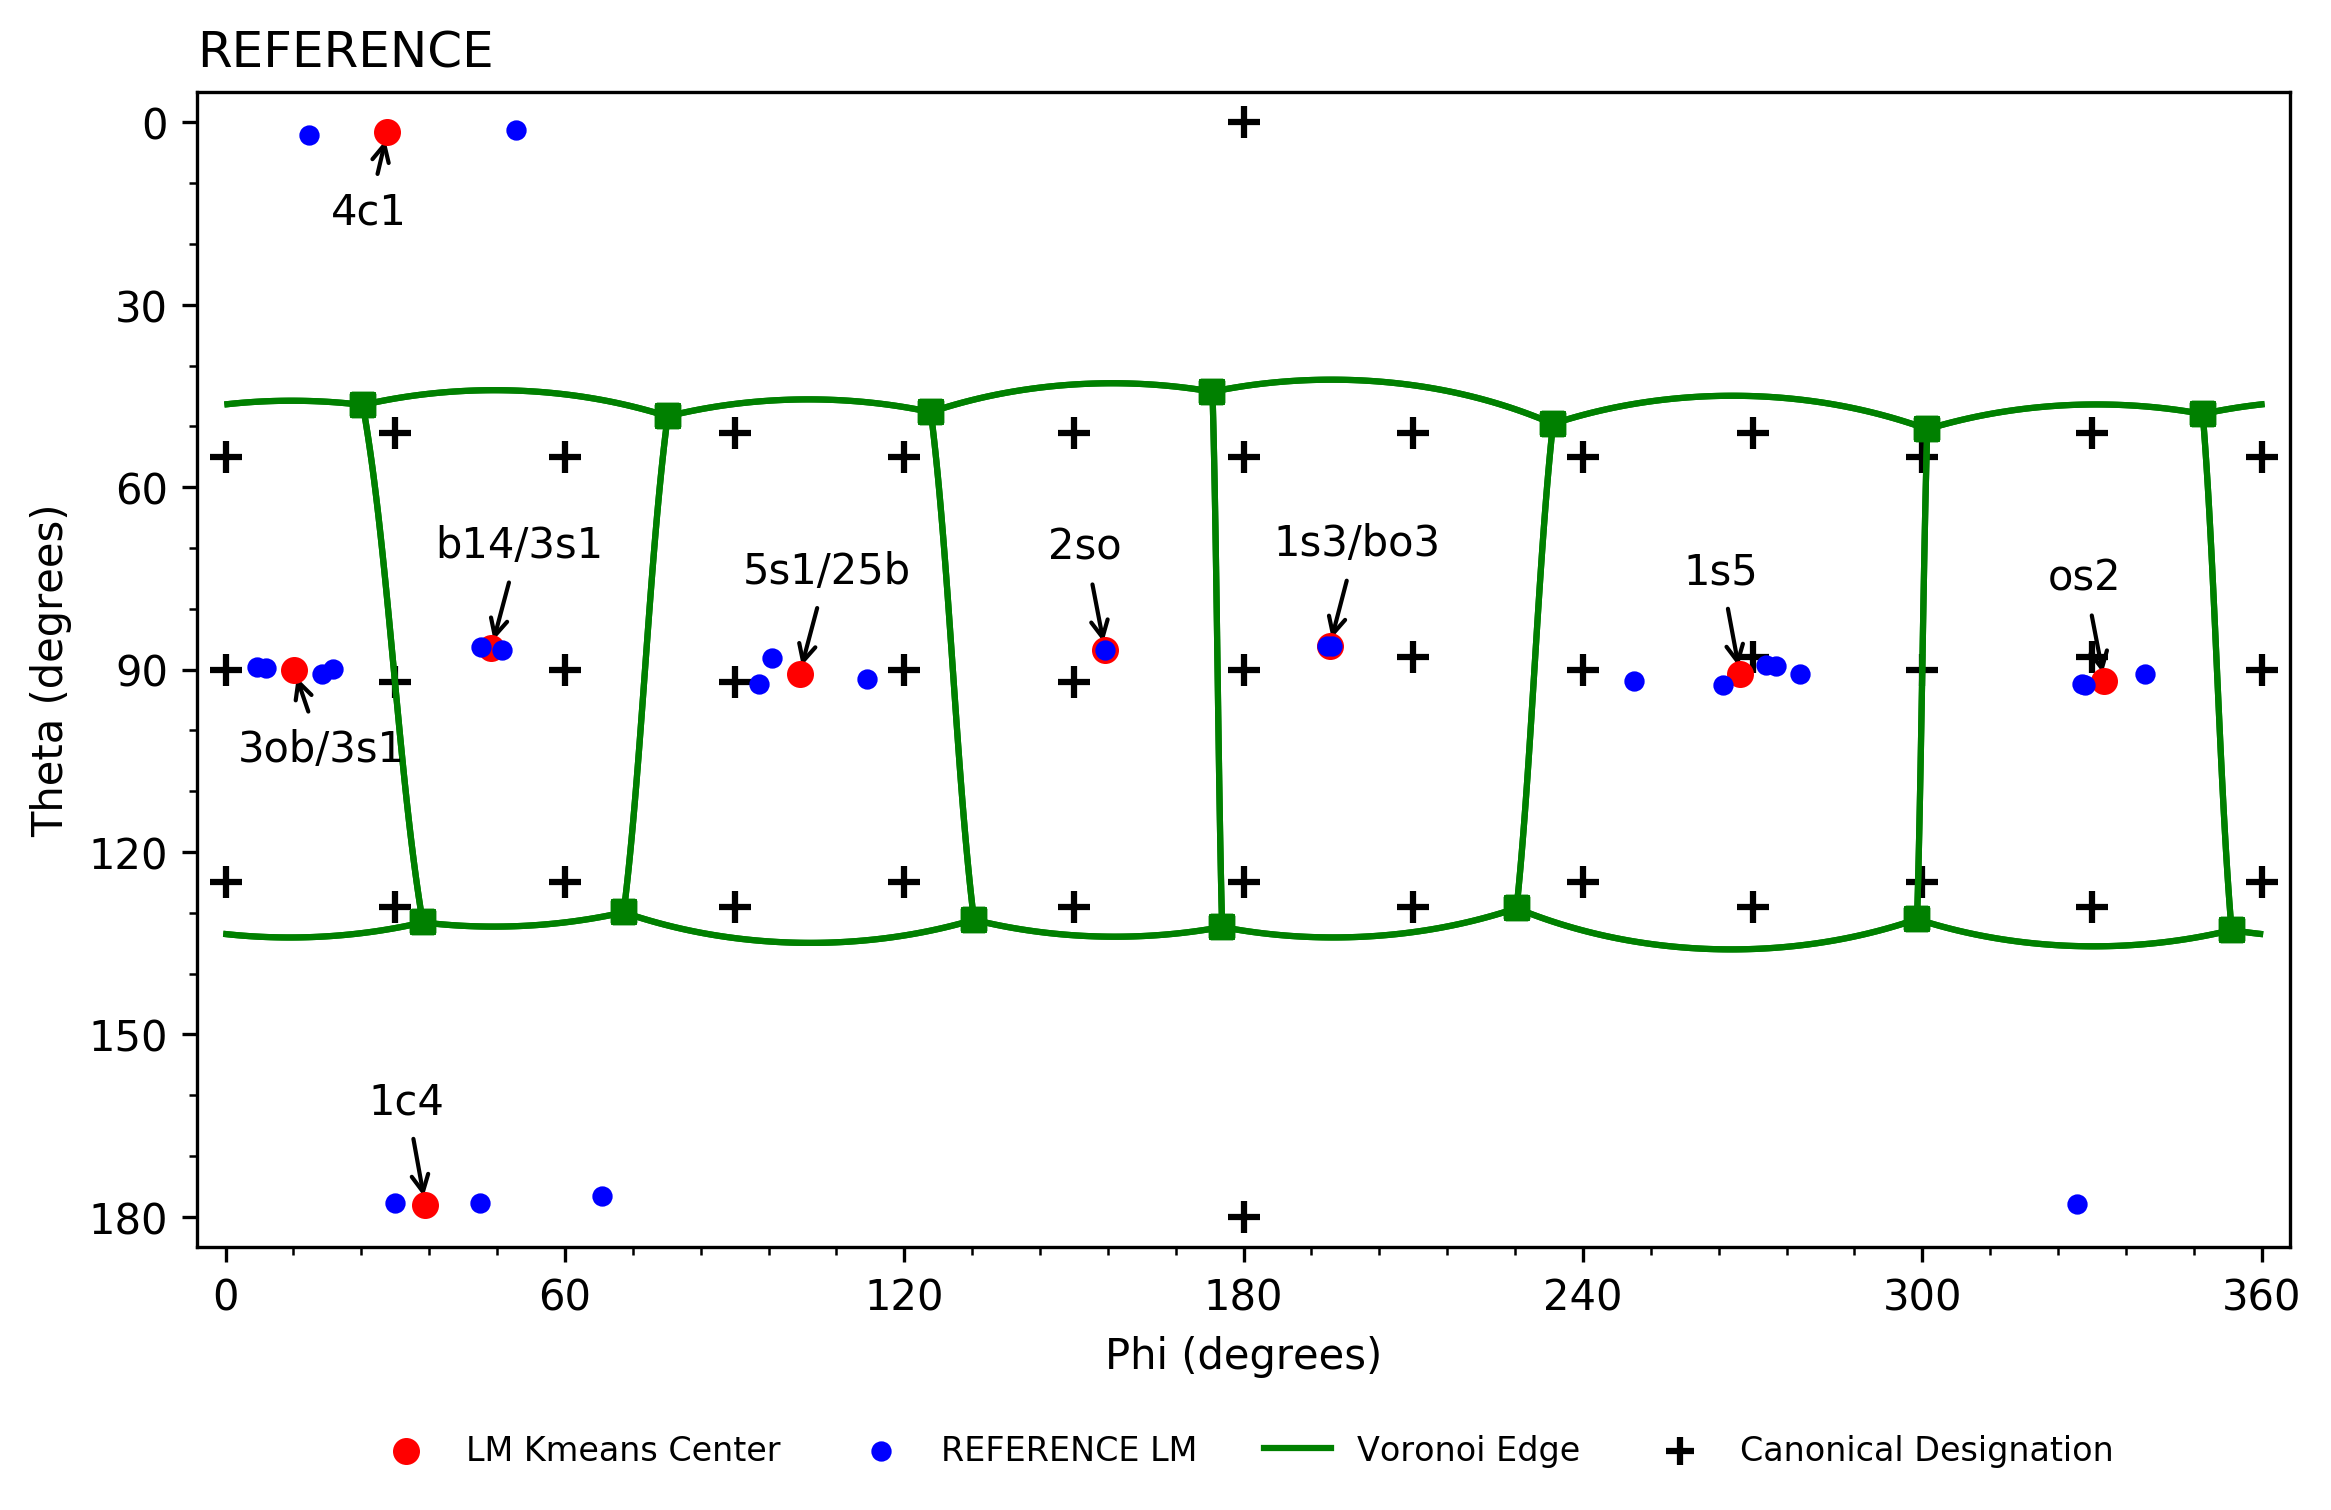
\includegraphics[width=\textwidth,height=\textheight,keepaspectratio]
	{figures/bxyl/overall/z_dataset-bxyl-LM-REFERENCE-all_groupings.png}
	\caption{The LM reference landscape for \textbeta-xylose. The reference structures (blue) are shown with the resulting k-means clustering
	centers (red).}
 	\label{fig:spherical_kmeans_lm}
\end{figure}

To compare the conformational landscapes generated by different methods, we utilized the 
conformational landscape generated by Mayes et al. \cite{Mayes2014} to assess the accuracy in producing stable local minima and transition state
ring geometries structures and pathways by a particular QM method. Rather than making comparisons based on the canonical designations, 
clustering algorithms were imposed on the CP parameters of the stable ring geometries of Mayes et al. to generate reference clusters. The reference
clusters served as the foundation for making comparisons between methods. For each molecule, a spherical k-means clustering algorithm\cite{Laska2016} 
was first applied to the Mayes et al. local minima, resulting in the local minima clusters for each molecule. Each spherical k-means
center was assigned a canonical designation to identify that particular group. Figure \ref{fig:spherical_kmeans_lm} demonstrates the final LM k-means 
cluster groups for \textbeta-xylose. The voronoi edges correspond to points that are equidistant from two LM k-means centers allowing for the tessellation 
to be visualized. 

Once the LM k-means centers were generated, the next phase involved clustering the TS on their associated LM. 
For a particular TS structure, the two LM were assigned to one of the LM k-means centers. The
same LM k-means cluster algorithm\cite{Laska2016} was then applied on each TS structure that connected two of the LM k-means 
centers (as shown in Figure \ref{fig:spherical_kmeans_TS_individual}). Figure \ref{fig:spherical_kmeans_TS_individual} demonstrates that three
unique pathways are available to convert between the 4c1 and 2so LM cluster groups. The same procedure was repeated for all possible combinations 
of LM groups to determine if there exists a pathway (or several) connecting the two. For a particular molecule, each of the LM k-mean centers 
and the TS k-mean centers can be found in the Supporting Information.

\begin{figure}[h!]
	\centering
	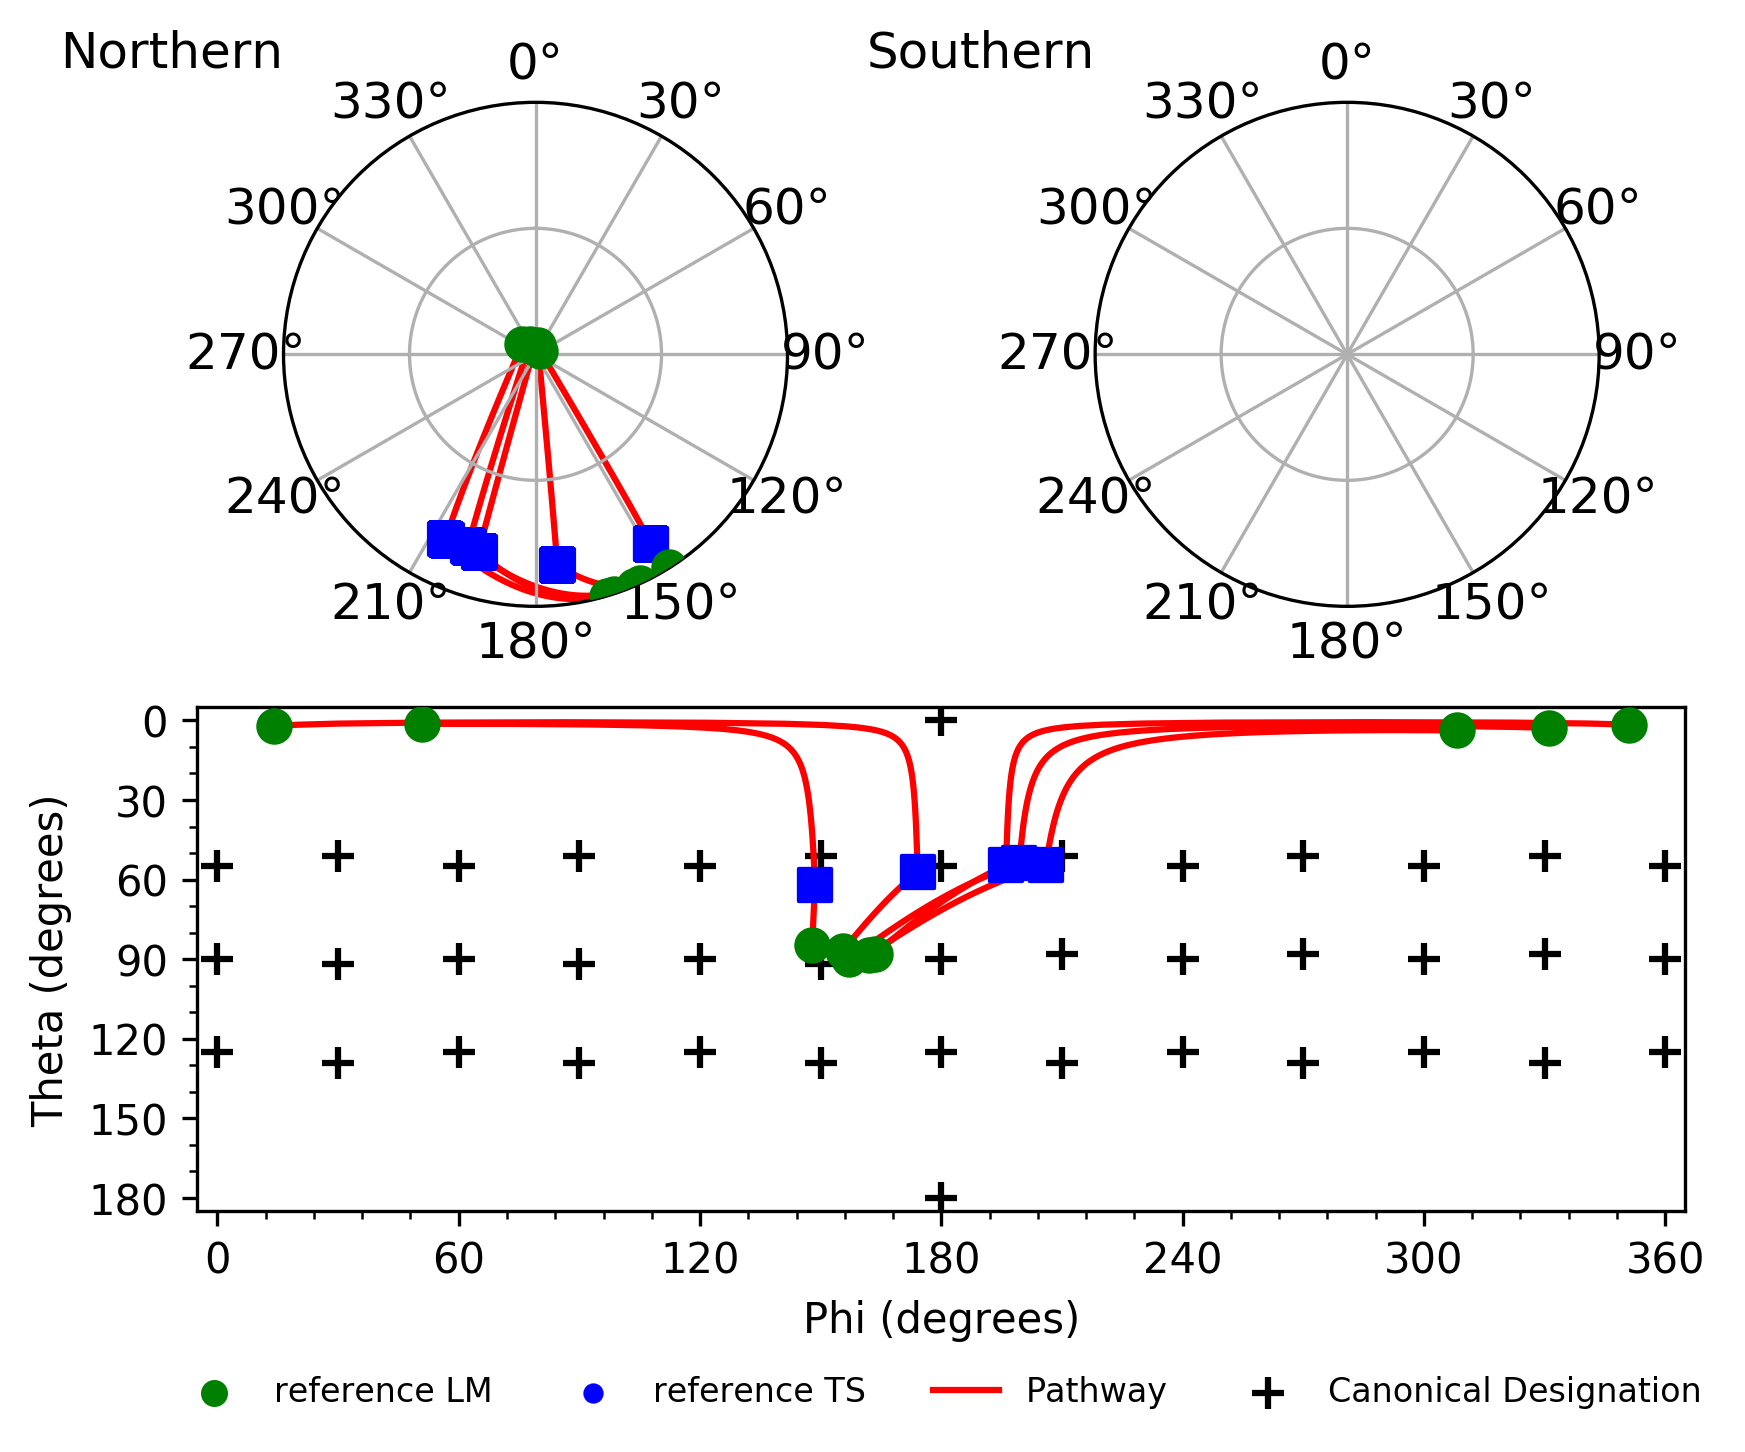
\includegraphics[width=\textwidth,height=\textheight,keepaspectratio]
	{figures/bxyl/z_dataset-bxyl-TS-reference-0_4.png}
	\caption{The TS reference landscape for \textbeta-xylose that connects the LM cluster groups 4c1 and 2so.}
	\label{fig:spherical_kmeans_TS_individual}
\end{figure}

\subsection{QM Calculations in Gaussian}
The conformational landscapes of oxane, \textbeta-xylose, and \textbeta-glucose were determined using Gaussian 09 rev D.01.\cite{Frisch2009} 
To compare the landscapes across different methods, a consistent screening procedure was developed and maintained for all calculations. 
Rather than performing a similar exhaustive search for all molecules using each proposed QM method, the final geometries of the Mayes et al. 
served as our initial starting geometries for our work on oxane, \textbeta-xylose, and \textbeta-glucose.\cite{Mayes2014} 
The initial procedure involved optimizing the benchmark structures to local minima and transition state at each of the proposed QM methods. 
Verification of the local minima and transition state structures was performed by viewing the imaginary frequencies: local minima have no imaginary 
frequencies while transition state (first order saddle point) structures have exactly one imaginary frequency. For consistency, an ultrafine integration 
grid and tight convergence criteria was set for each method. For all DFT methods, a basis set of 6$-$31+G(d,p) was specified. The 6$-$31+G(d,p) 
basis set was selected for its polarization functions on all atoms and diffuse function on hydrogen atoms. Subsequent frequency calculations were 
performed to determine the thermodynamic quantities associated with each local minima and transition state structure. Python (\hl{REFERENCE}) 
scripts were created to identify unique local minima and transition structures based on root mean square difference (RMSD) and dipole differences 
between structures. Duplicate local minima and transition state structures were removed to focus on unique structures and reduce computational cost. 
	
The next phase of the screening process involved determining whether or not the transition state was a ring-puckering or exo-cyclic transition state 
using normal mode analysis in Gaussian.\cite{Frisch2009} Ring-puckering transition states were determined if the ring dihedral contribution to the 
imaginary normal mode exceeded a specific tolerance value. A definitive distinction between ring-puckering or exo-cyclic transition states was visible 
upon analysis of the contributions. Additionally, structures were checked using ChemCraft to visually verify the ring-puckering designation.\cite{ChemCraft}
The exo-cyclic transition states were removed from further analysis to focus on the interconversion pathways between puckers. With the ring-puckering 
transition states identified, intrinsic reaction coordinate (IRC) calculations were performed to find the pathways interconnecting local minima through a 
particular transition state. 


\subsection{Comparison Metrics}
\begin{outline}[enumerate]
The conformational landscape generated by each QM method was compared to the extensive, benchmark conformational 
landscape by Mayes et al. The following metrics were used to quantify difference in conformation (structure) and energy for 
the various landscapes.
\1 Root mean square difference (RMSD) within a cluster group.
	\2 Quantifies the variation in the structures generated by a particular method to the benchmark structures based solely 
	on CP parameters. This method is less than ideal since the energy of the structures are not incorporated into
	the calculation. 
	\2 Equation:
	$$
		RMSD=\sum_{i=1}^{N} \frac{(d_i)^2}{N}
	$$
	where $i$ is one of $N$  structures located within a particular clustering group and $d$ is the arc length between point $i$
	and the k-means cluster center. 
\1 Weighted root mean square difference (WRMSD) with a cluster group.
	\2 Quantifies the variation in the structures generated by a particular method to the benchmark structures based on the CP
	parameters and the energy of the structures. Low energy structures that are closer to the benchmark k-mean center 
	are rewarded, whereas low energy structures that are further away from the benchmark k-mean center are penalized. 
	\2 Equation: 
	$$
		WRMSD=\sum_{i=1}^{N} \frac{W_i(d_i)^2}{N}
	$$
	where $i$ is one of $N$  structures located within a particular clustering group, $d$ is the arc length for structure $i$
	and the k-means cluster center, and $W_i$ is the Boltzmann weighting factor for structure $i$.
\1 Boltzmann Weighted Relative Gibbs Free Energies
	\2 Calculation for the Boltzmann Weighted Relative Gibbs Free energies within each cluster group.
	\2 Equation:
	$$
		\Delta G_W = \sum_{i=1}^{N} \Delta G_i W_i =  \sum_{i=1}^{N} \Delta G_i \Bigg(\frac{e^{\frac{-\Delta G_i}{k_B T}}}{\sum_{j=1}^{N}e^{\frac{-\Delta G_j}{k_B T}}}\Bigg)
	$$
	where $\Delta G_i$ relative Gibbs Free energy for structure $i$, $k_B$ is Boltzmann's constant, $T$ is the temperature (in Kelvin), 
	$\Delta G_j$ is the relative Gibbs Free energy for structure $j$ of $N$ structures within the cluster group. 
\1 Root mean square difference within a cluster group (based on the Weighted Boltzmann Relative Gibbs Free energies)
	\2 Quantifies the variation in the predicted Gibbs Free Energies to the reference Gibbs Free energies (within each cluster group).    
	\2 Equation: 
	$$ 
		GRMSD=\sum_{i=1}^{N} \frac{(\Delta G_{W_i} - \Delta G_{REF_i})^2}{N}
	$$ 
	where $\Delta G_{W_i}$ is the weighted Gibbs Free Energy for the $i$ cluster group, $\Delta G_{REF_i}$ is the reference Gibbs Free
	Energy for the $i$ cluster group, and $N$ represents the total number of clusters. Note that the RMSD calculations only incorporate 
	matches; all false positives (the QM method finds a structure that the reference method missed) and false negatives (the QM method
	missed a structure that the reference method contains) are removed from the calculation. 	
\end{outline}



%%%%%%%%%%%%%%%%%%%%%%%%%%%%%%%%%%%%%%%%%%%%%%%%%%%%%%%%%%%%%%%%%%%%%%%%
% 										         PRELIMINARY RESULTS                                                                                             %
%%%%%%%%%%%%%%%%%%%%%%%%%%%%%%%%%%%%%%%%%%%%%%%%%%%%%%%%%%%%%%%%%%%%%%%%
\newpage
\section{Preliminary Results}

% % % % % % % % % 
% % % Oxane  % % % 
% % % % % % % % % 
\subsection{Oxane}
Oxane, the simplest pyranose ring, served as the foundation for our conformational investigation since it contains no exo-cyclic groups. All 
calculations were initial perform on oxane, and then expanded to the other molecules in our investigation.

\subsubsection{Local Minima Reference Landscape}
To compare the conformational landscapes across different methods, we initially generated a set of reference landscapes based on the work
of Mayes et al. (as discussed in the Computational Methods: Generating Reference Landscapes section). Figure \ref{fig:oxane-ref-LM} shows 
the LM k-mean centers (red) for the reference structures as well as the voronoi edges (green) and the raw data from Mayes et al. (blue). 

\begin{figure}[h!]
  	\centering
  	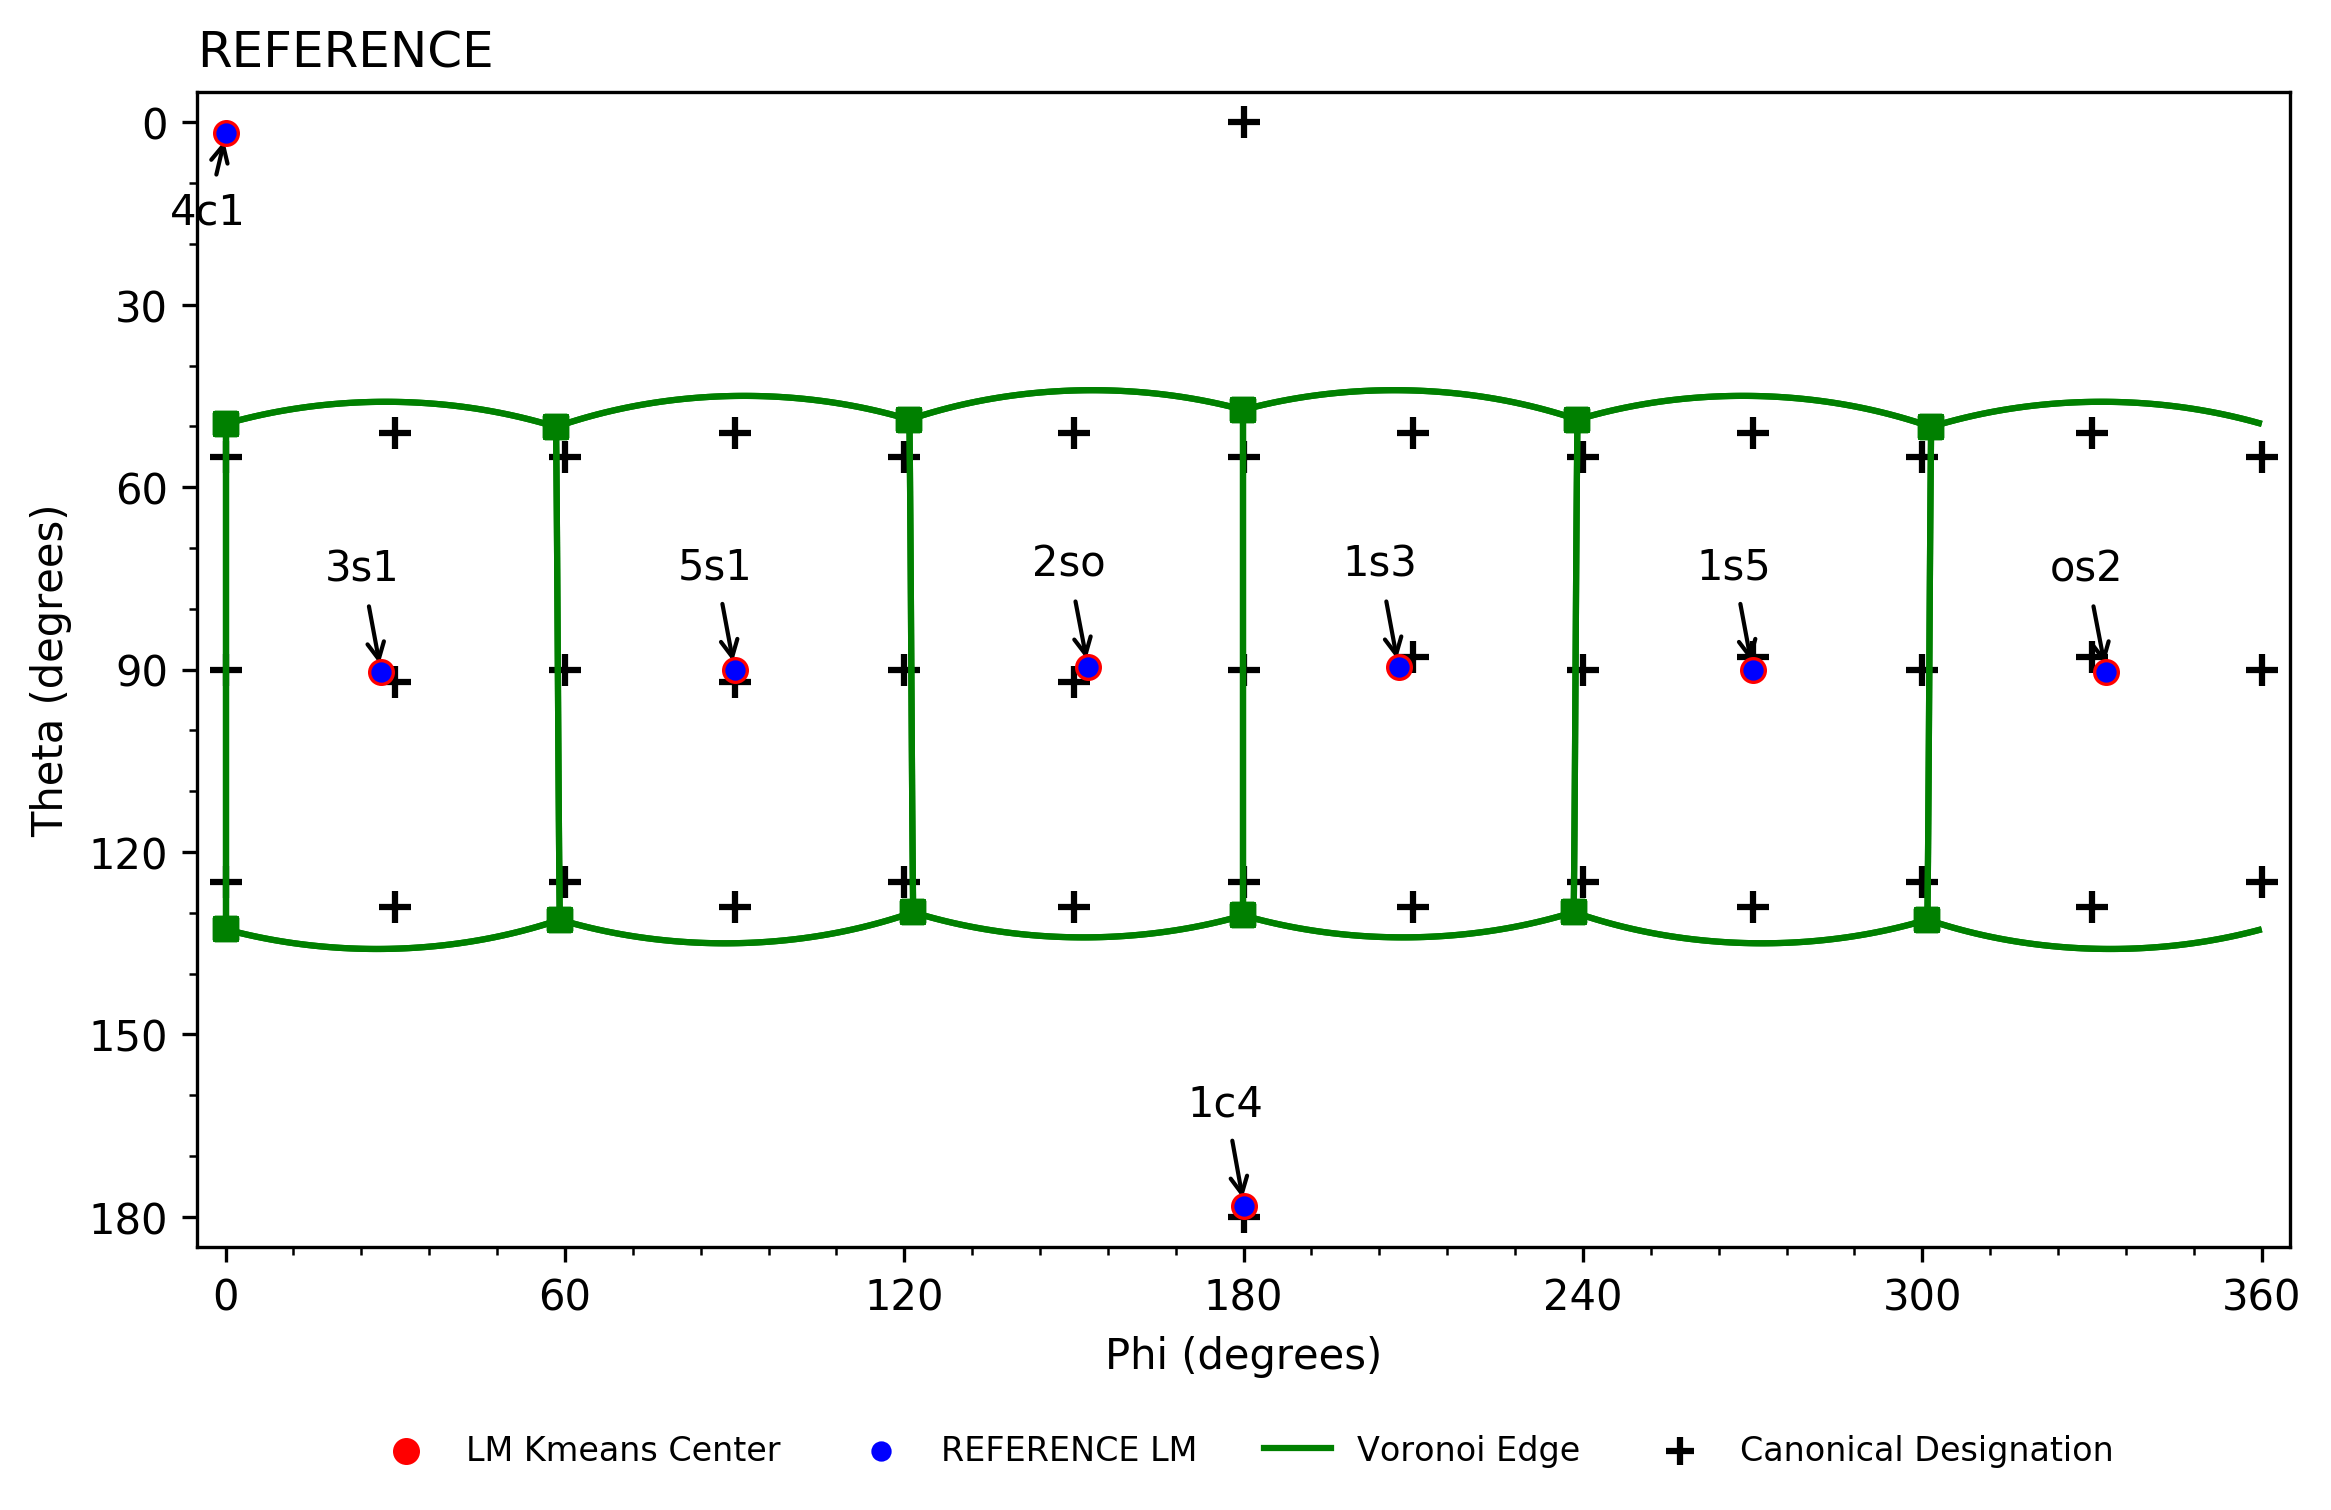
\includegraphics[width=\textwidth,height=\textheight,keepaspectratio]
	{figures/oxane/overall/z_dataset-oxane-LM-REFERENCE-all_groupings.png}
	\caption{The LM reference landscape for oxane.}
 	\label{fig:oxane-ref-LM}
\end{figure}

\subsubsection{Transition State Reference Landscape}
With the LM conformational landscape for oxane generated, the TS connecting each LM were then determined. Each TS found in Figure
\ref{fig:oxane-ref-TS} represents a unique structure that connects two LM. To aid in visualization, Northern and Southern hemisphere plots
were created to highlight key pathways from 4c1 and 1c4 conformations.

\begin{figure}[H]
  	\centering
  	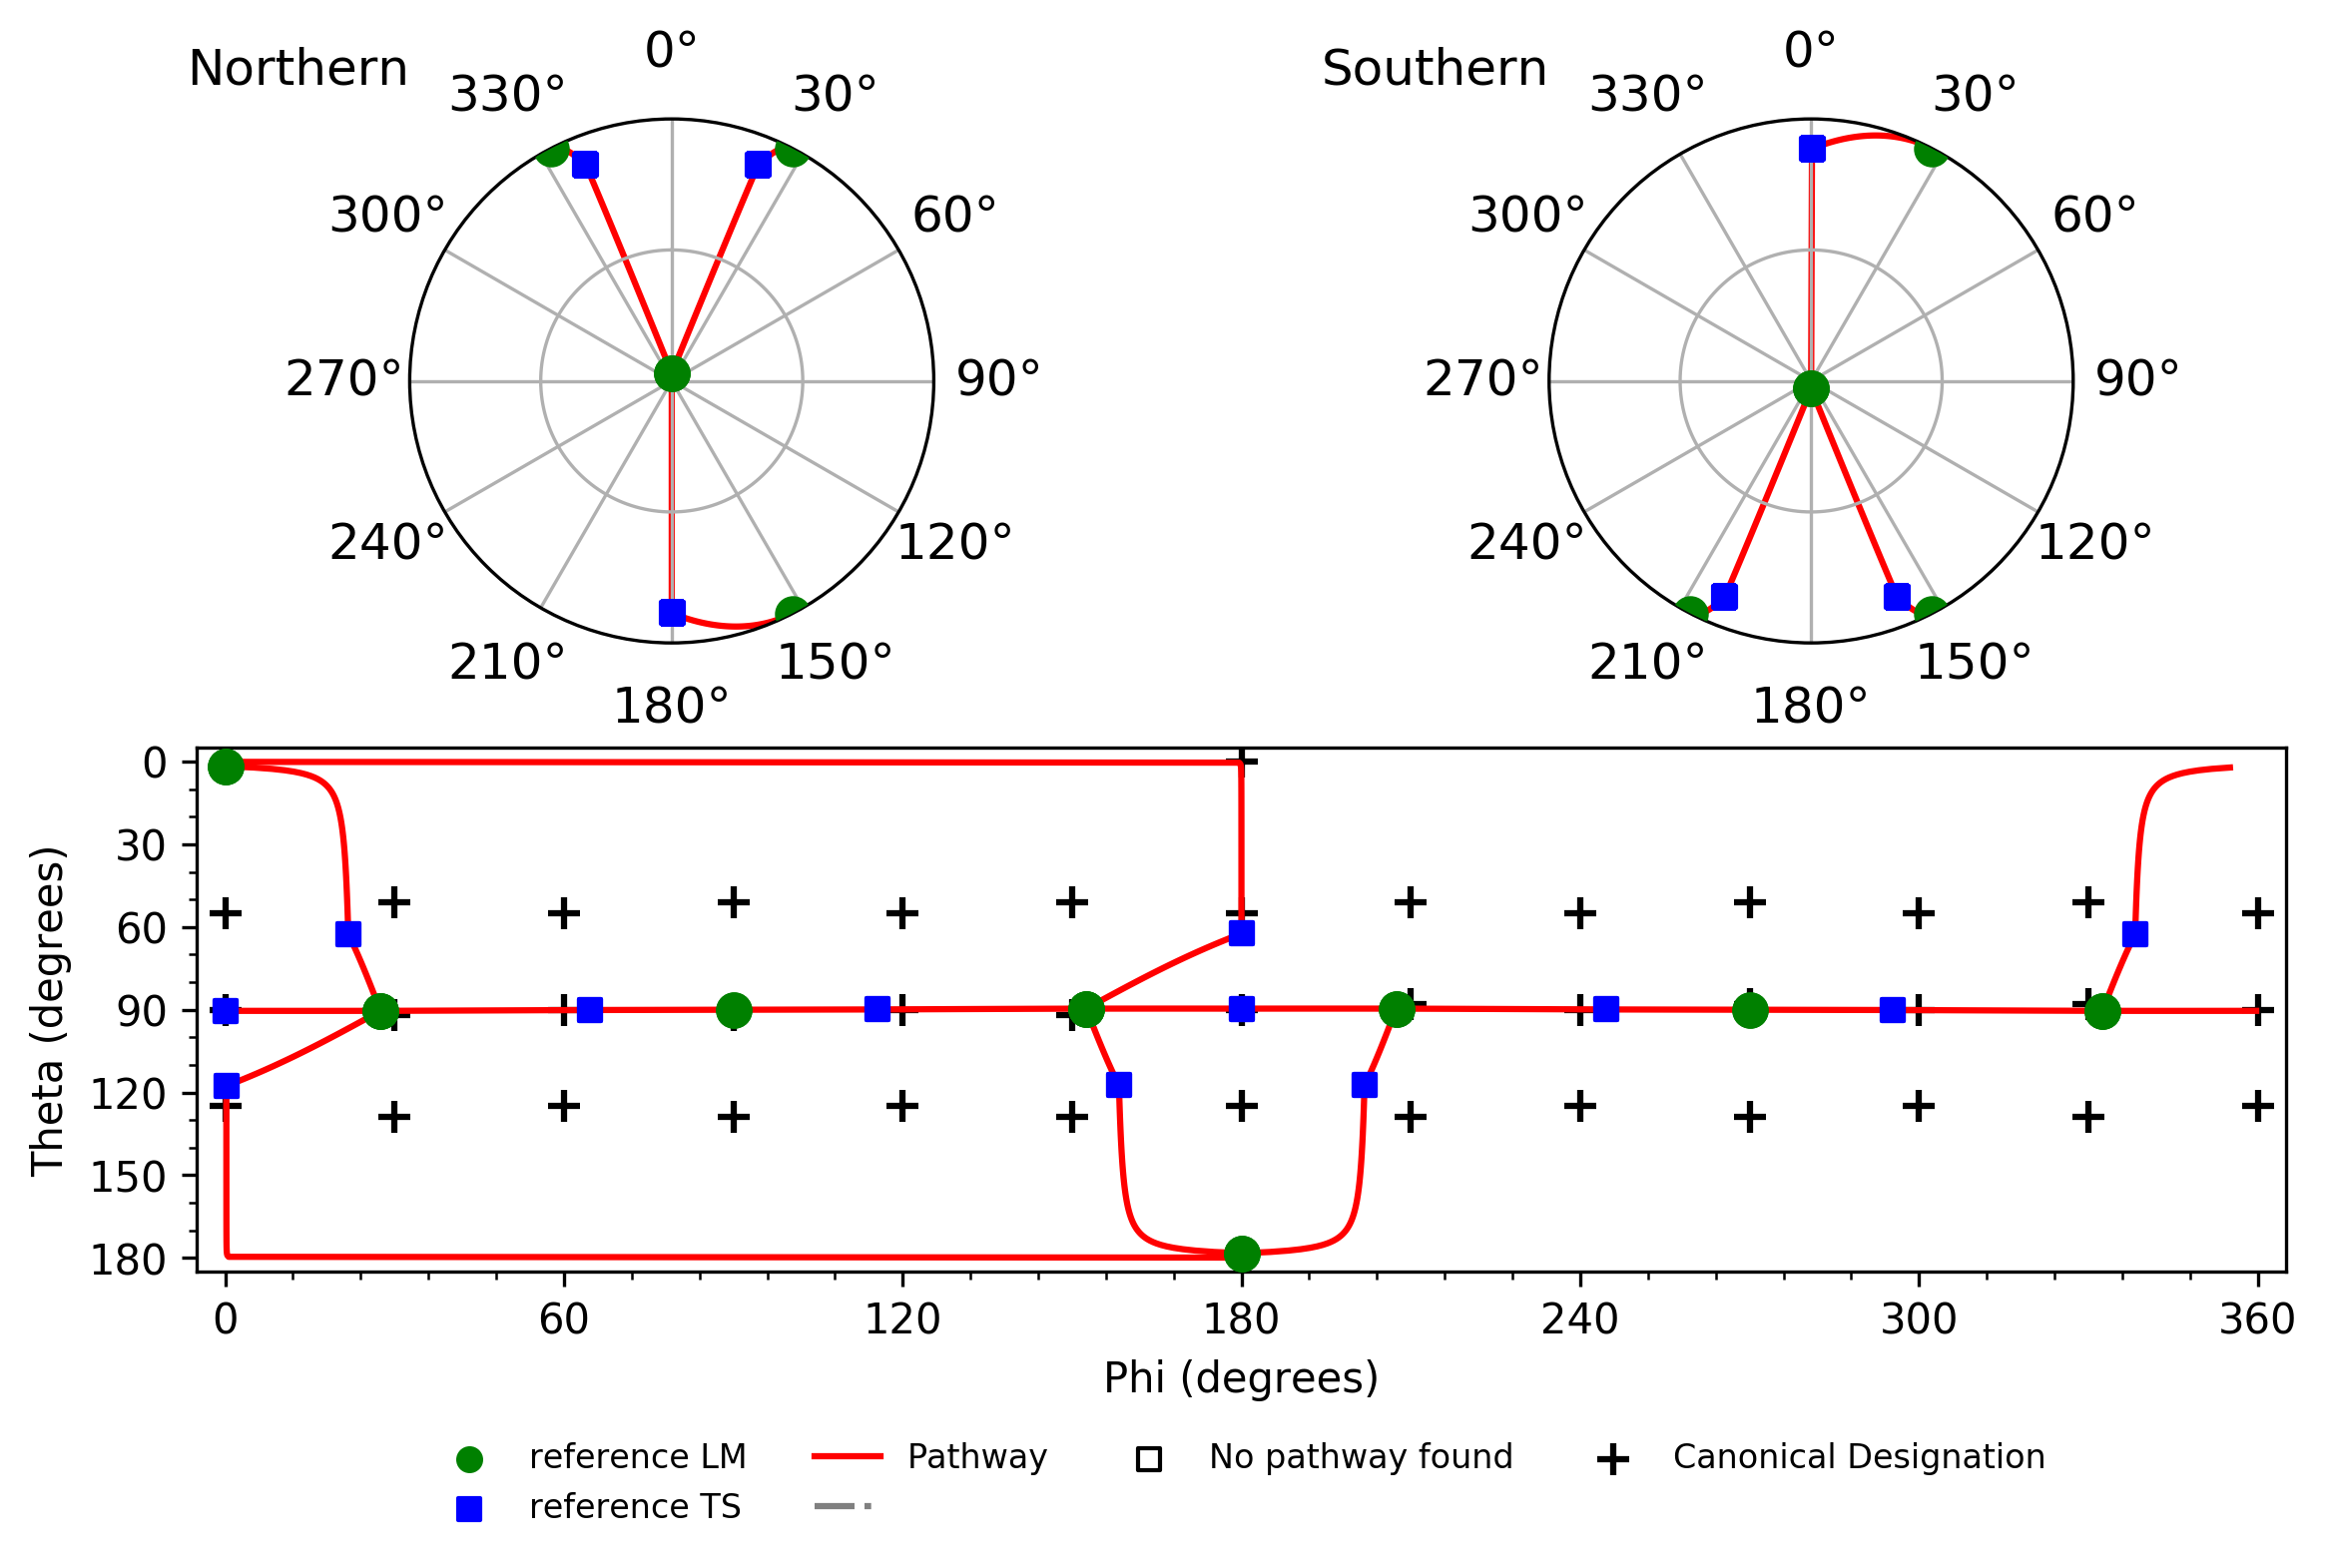
\includegraphics[width=\textwidth,height=\textheight,keepaspectratio]
	{figures/oxane/z_dataset-oxane-TS-heatmap-reference.png}
	\caption{The TS reference landscape for oxane.}
 	\label{fig:oxane-ref-TS}
\end{figure}


\subsubsection{Local Minima Landscapes}

\begin{figure}[H]
	\centering
   	\begin{subfigure}[b]{0.49\textwidth}
   	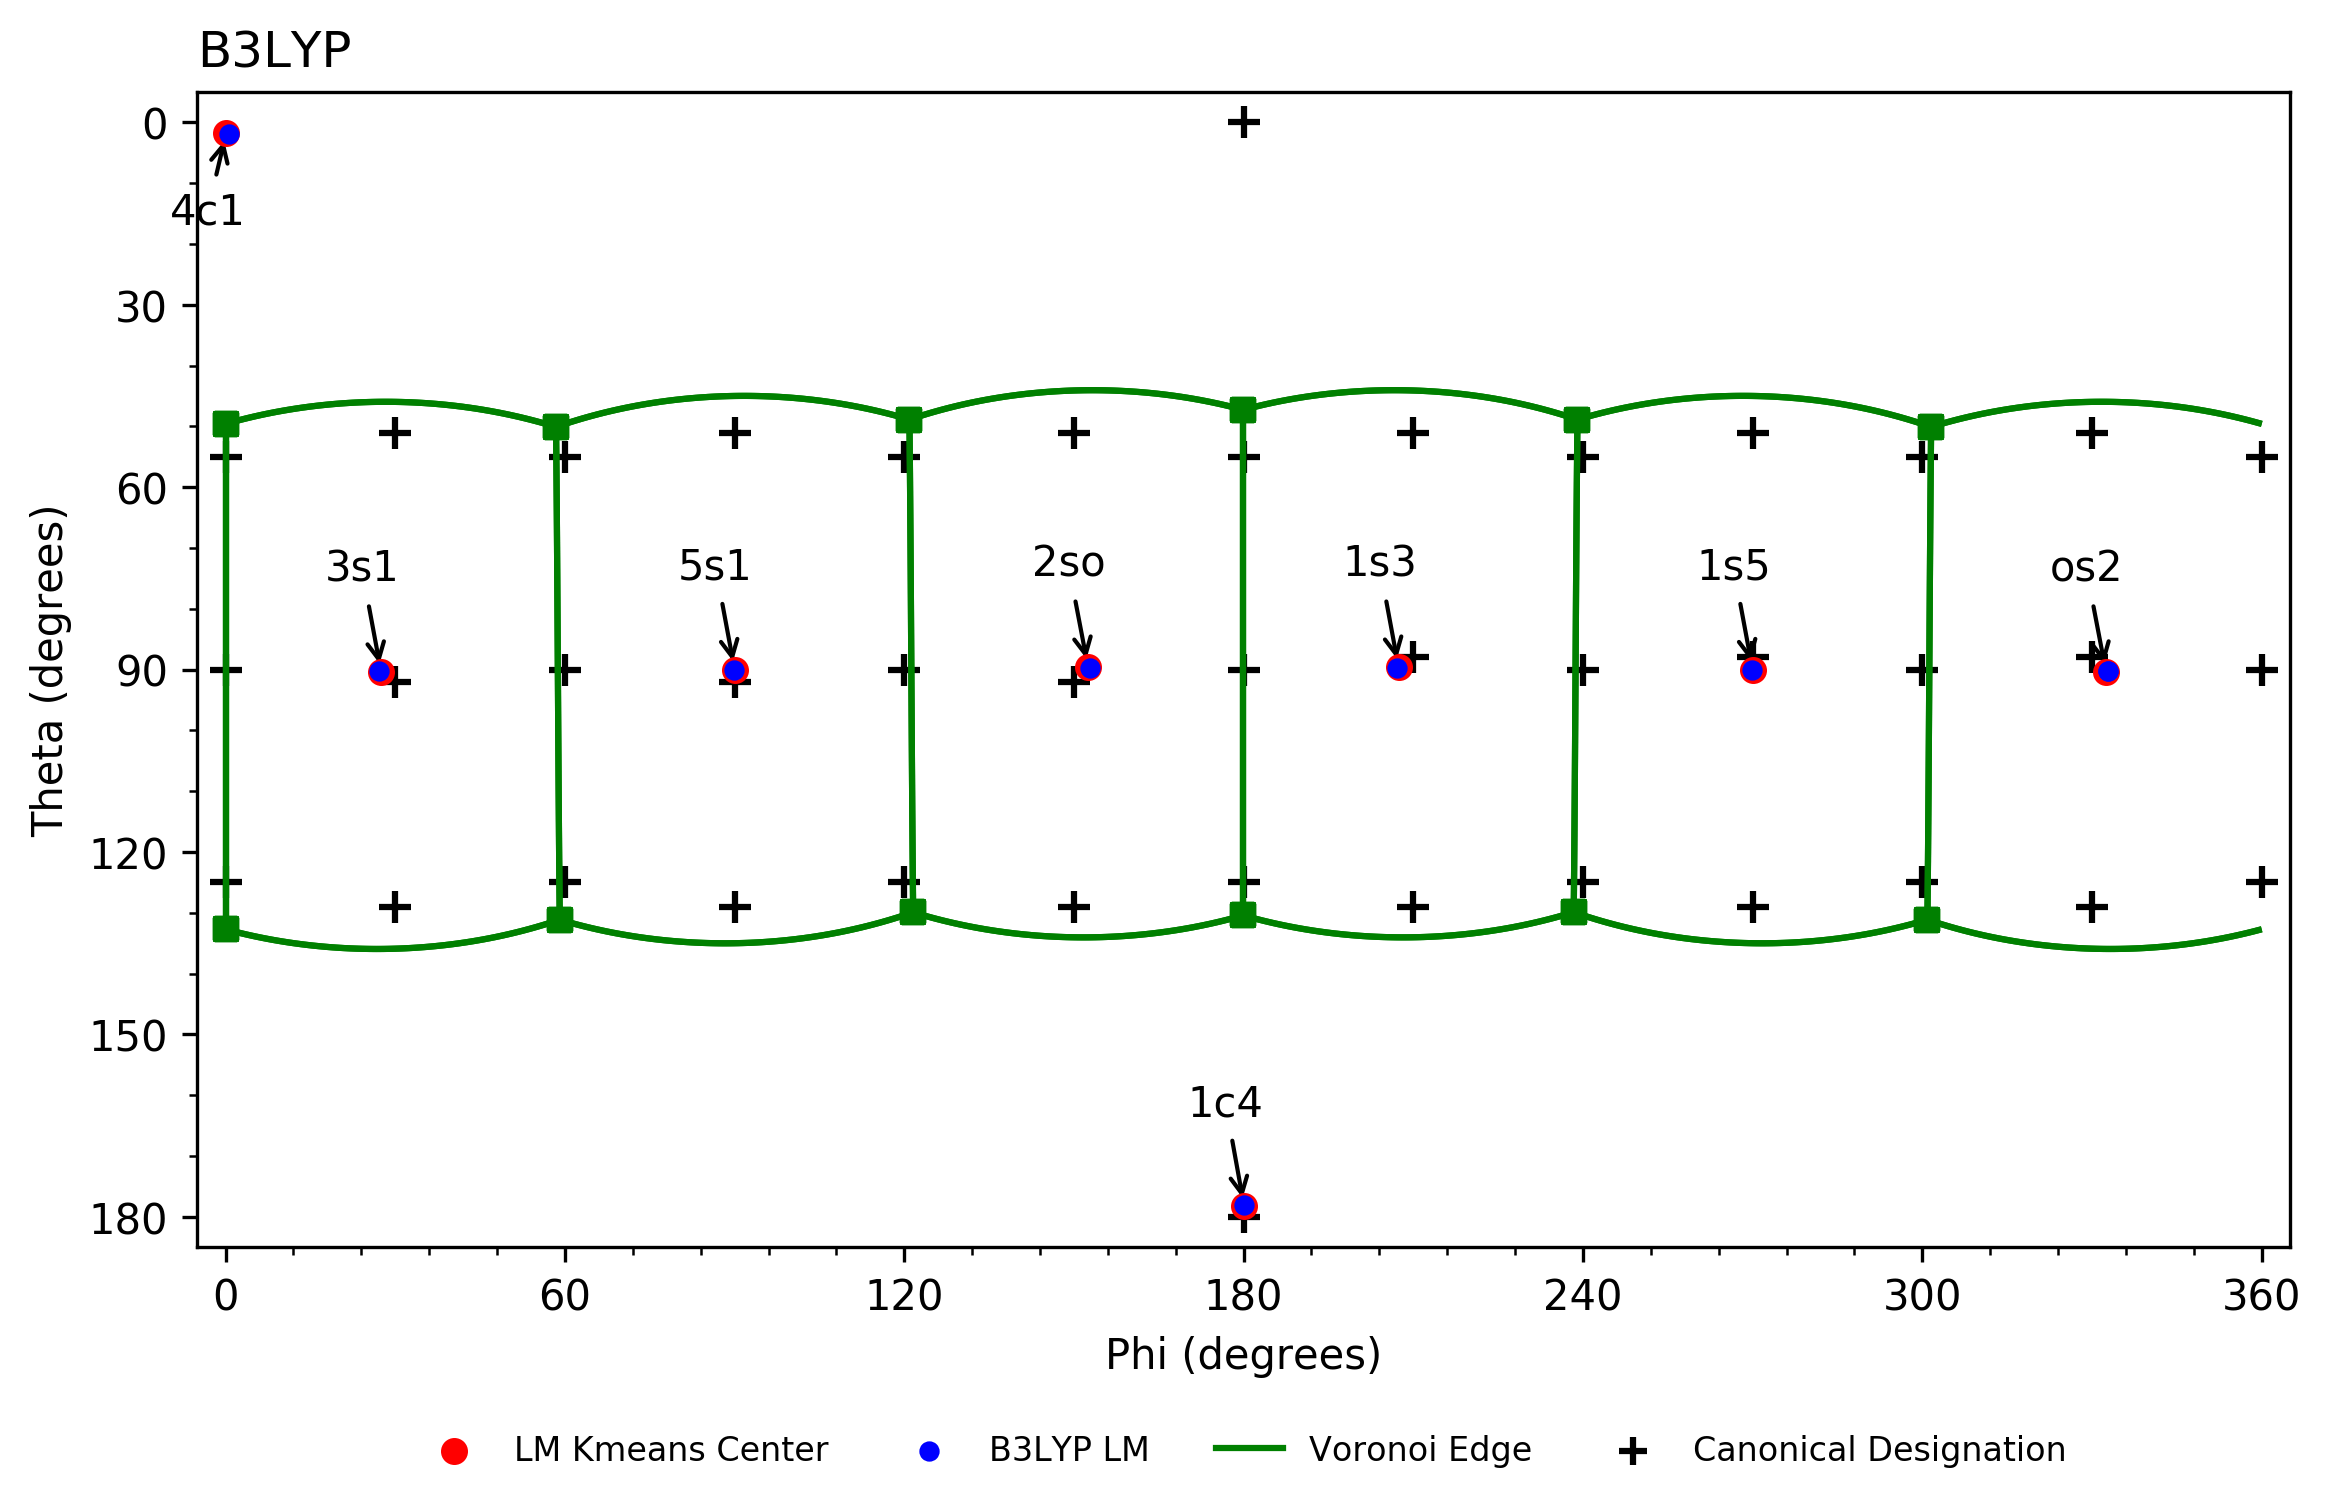
\includegraphics[width=1\textwidth,keepaspectratio]
   	{figures/oxane/overall/z_dataset-oxane-LM-B3LYP-all_groupings.png}
   	\caption{B3LYP/6$-$31+G(d,p)}
	\end{subfigure}
	~
	\begin{subfigure}[b]{0.49\textwidth}
	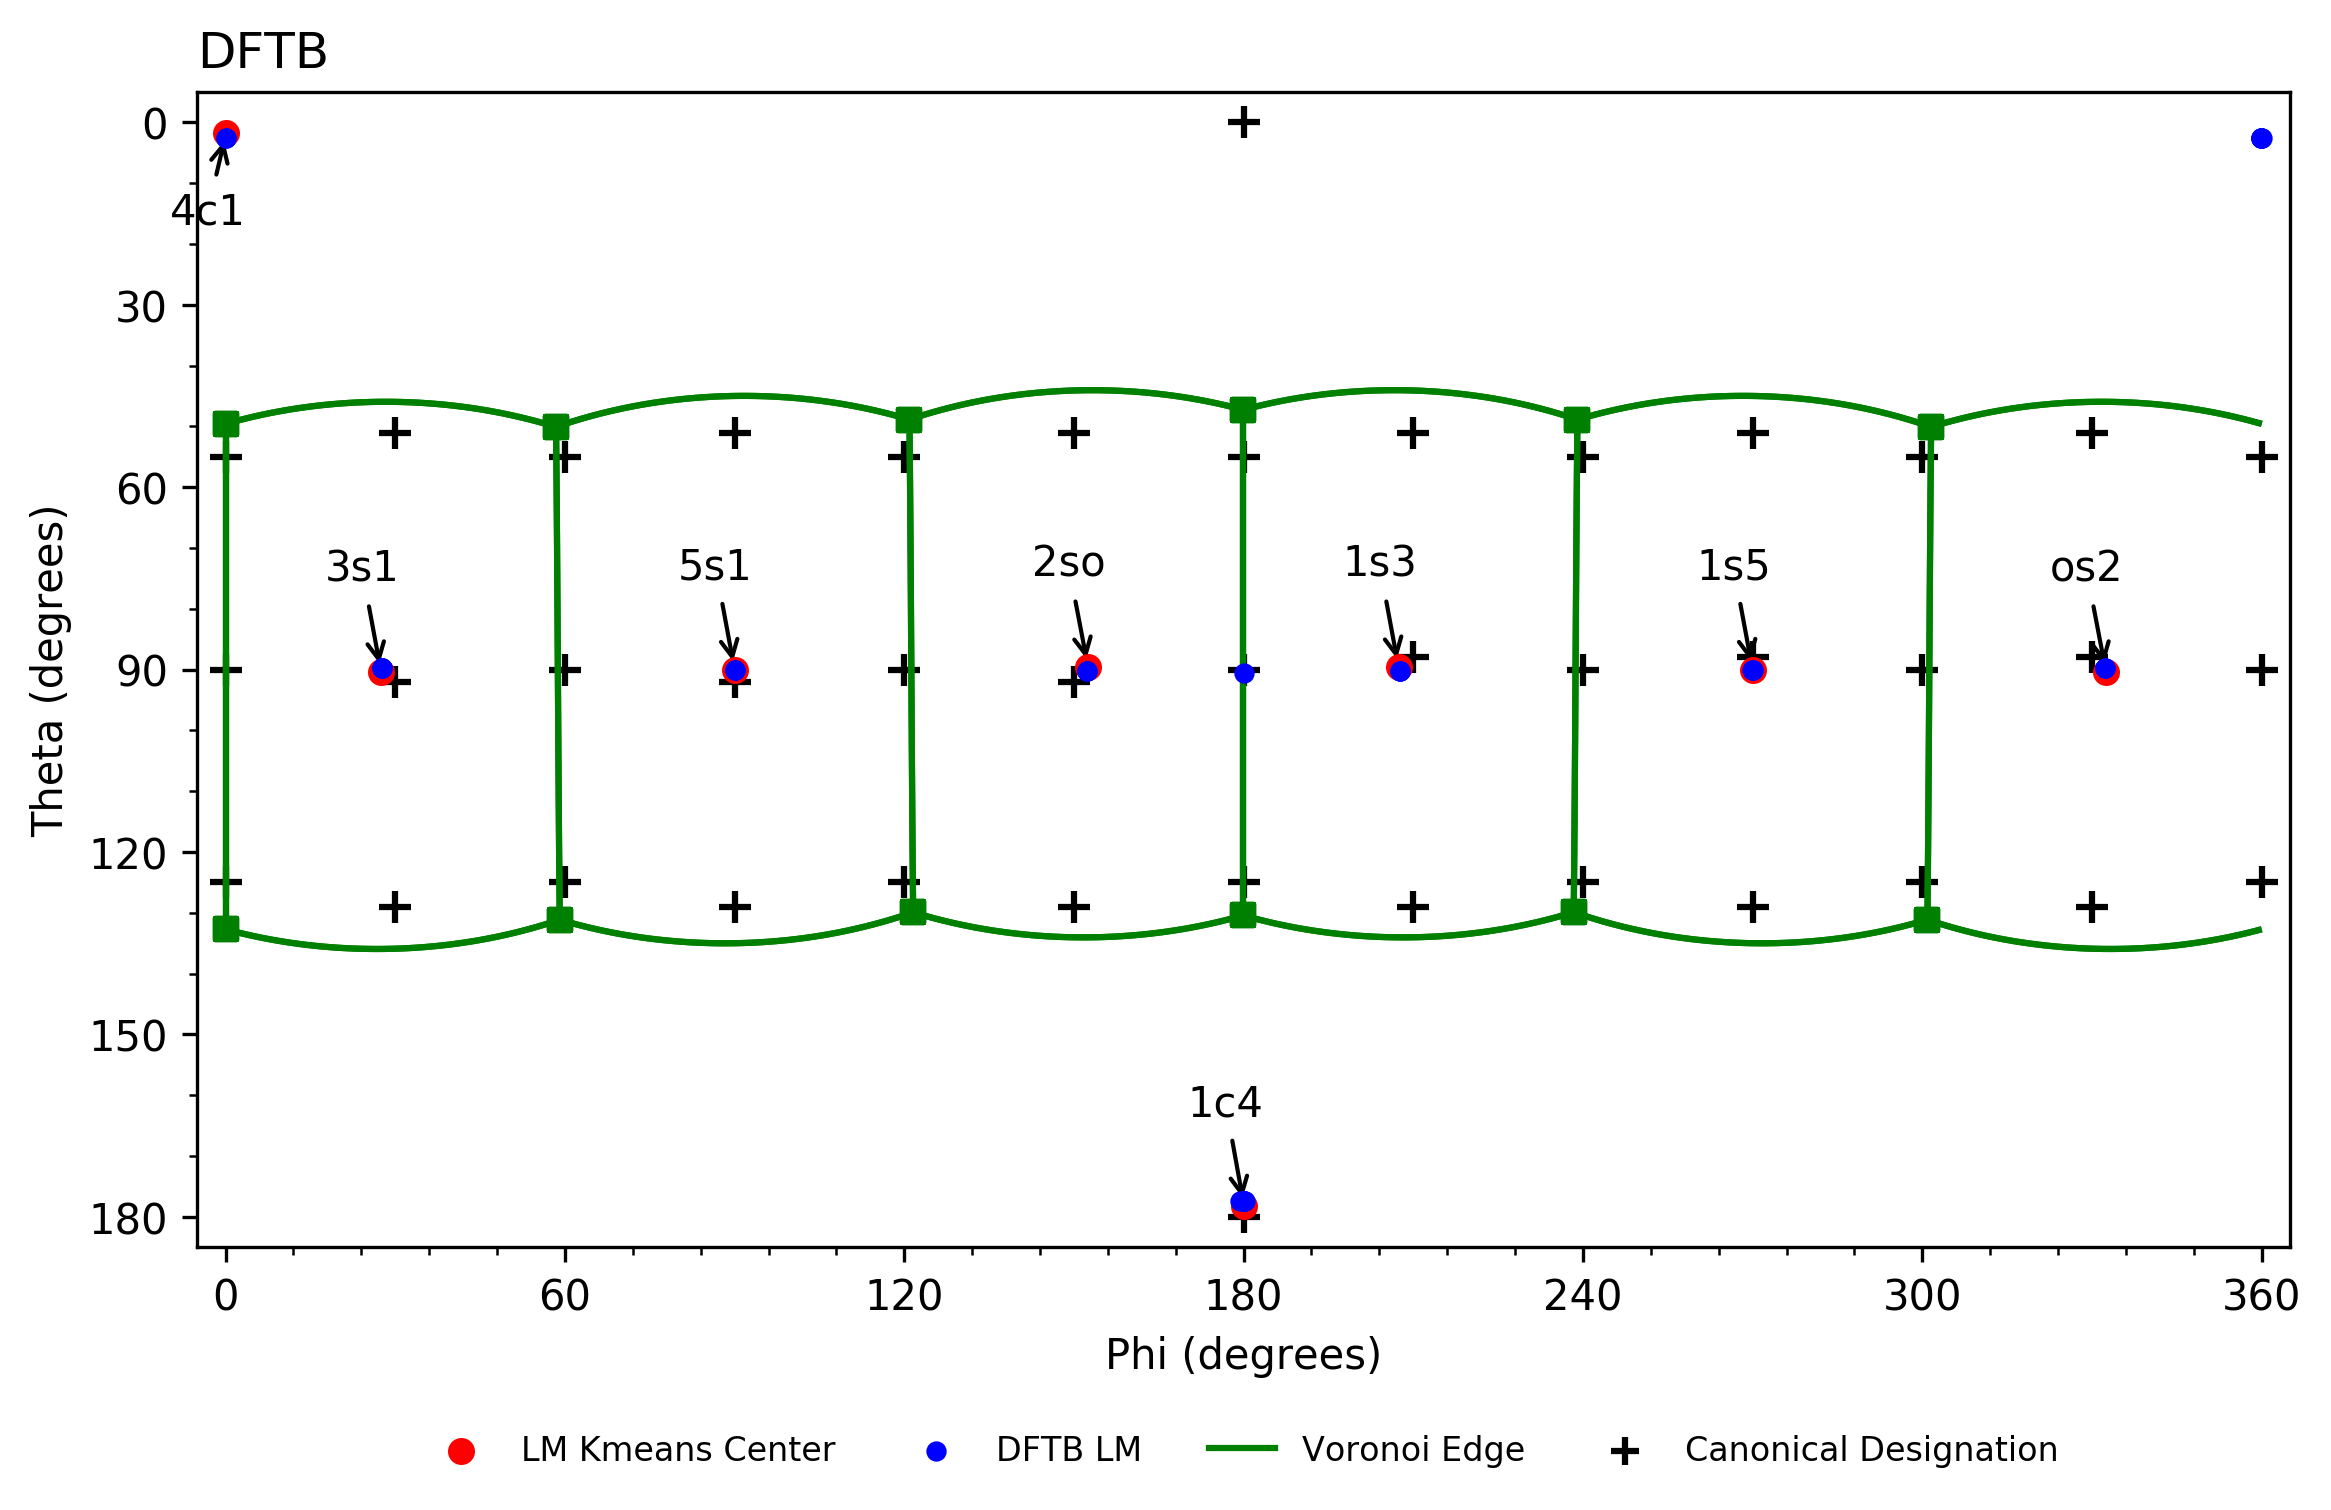
\includegraphics[width=1\textwidth,keepaspectratio]
   	{figures/oxane/overall/z_dataset-oxane-LM-DFTB-all_groupings.png}
	\caption{DFTB}
	\end{subfigure}
\end{figure}

\begin{figure}[H]\ContinuedFloat
	\centering
   	\begin{subfigure}[b]{0.49\textwidth}
   	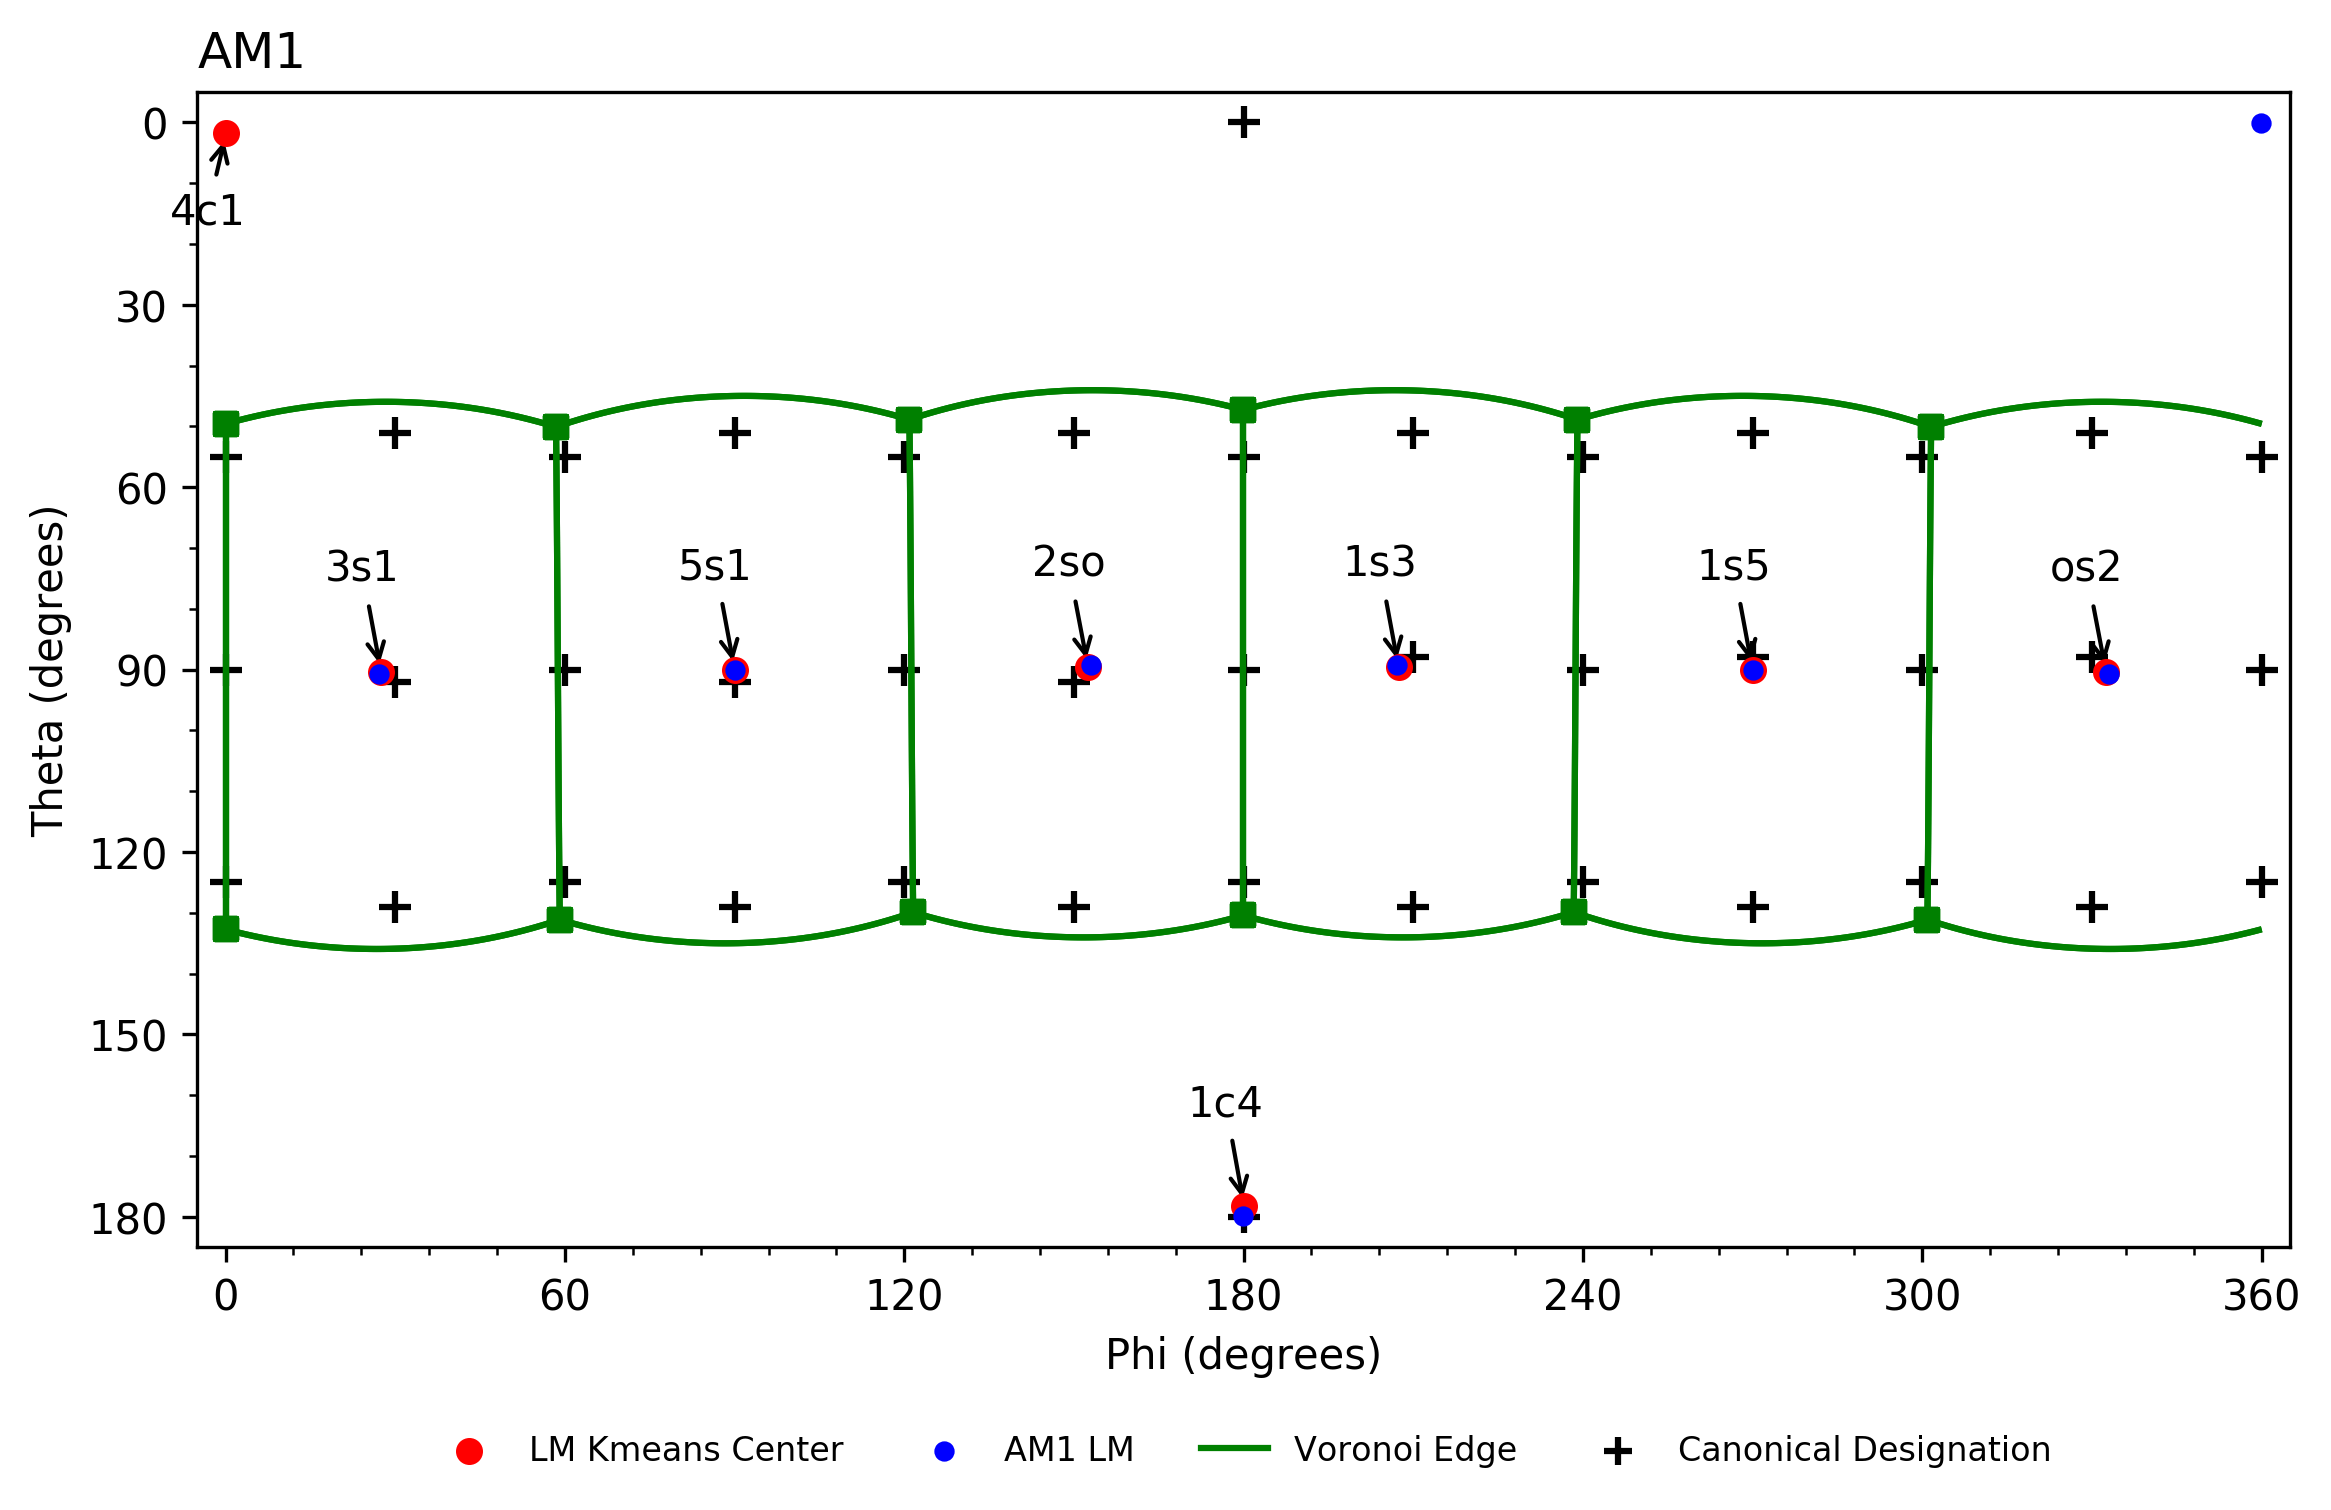
\includegraphics[width=1\textwidth,keepaspectratio]
   	{figures/oxane/overall/z_dataset-oxane-LM-AM1-all_groupings.png}
   	\caption{AM1}
	\end{subfigure}
	~
	\begin{subfigure}[b]{0.49\textwidth}
	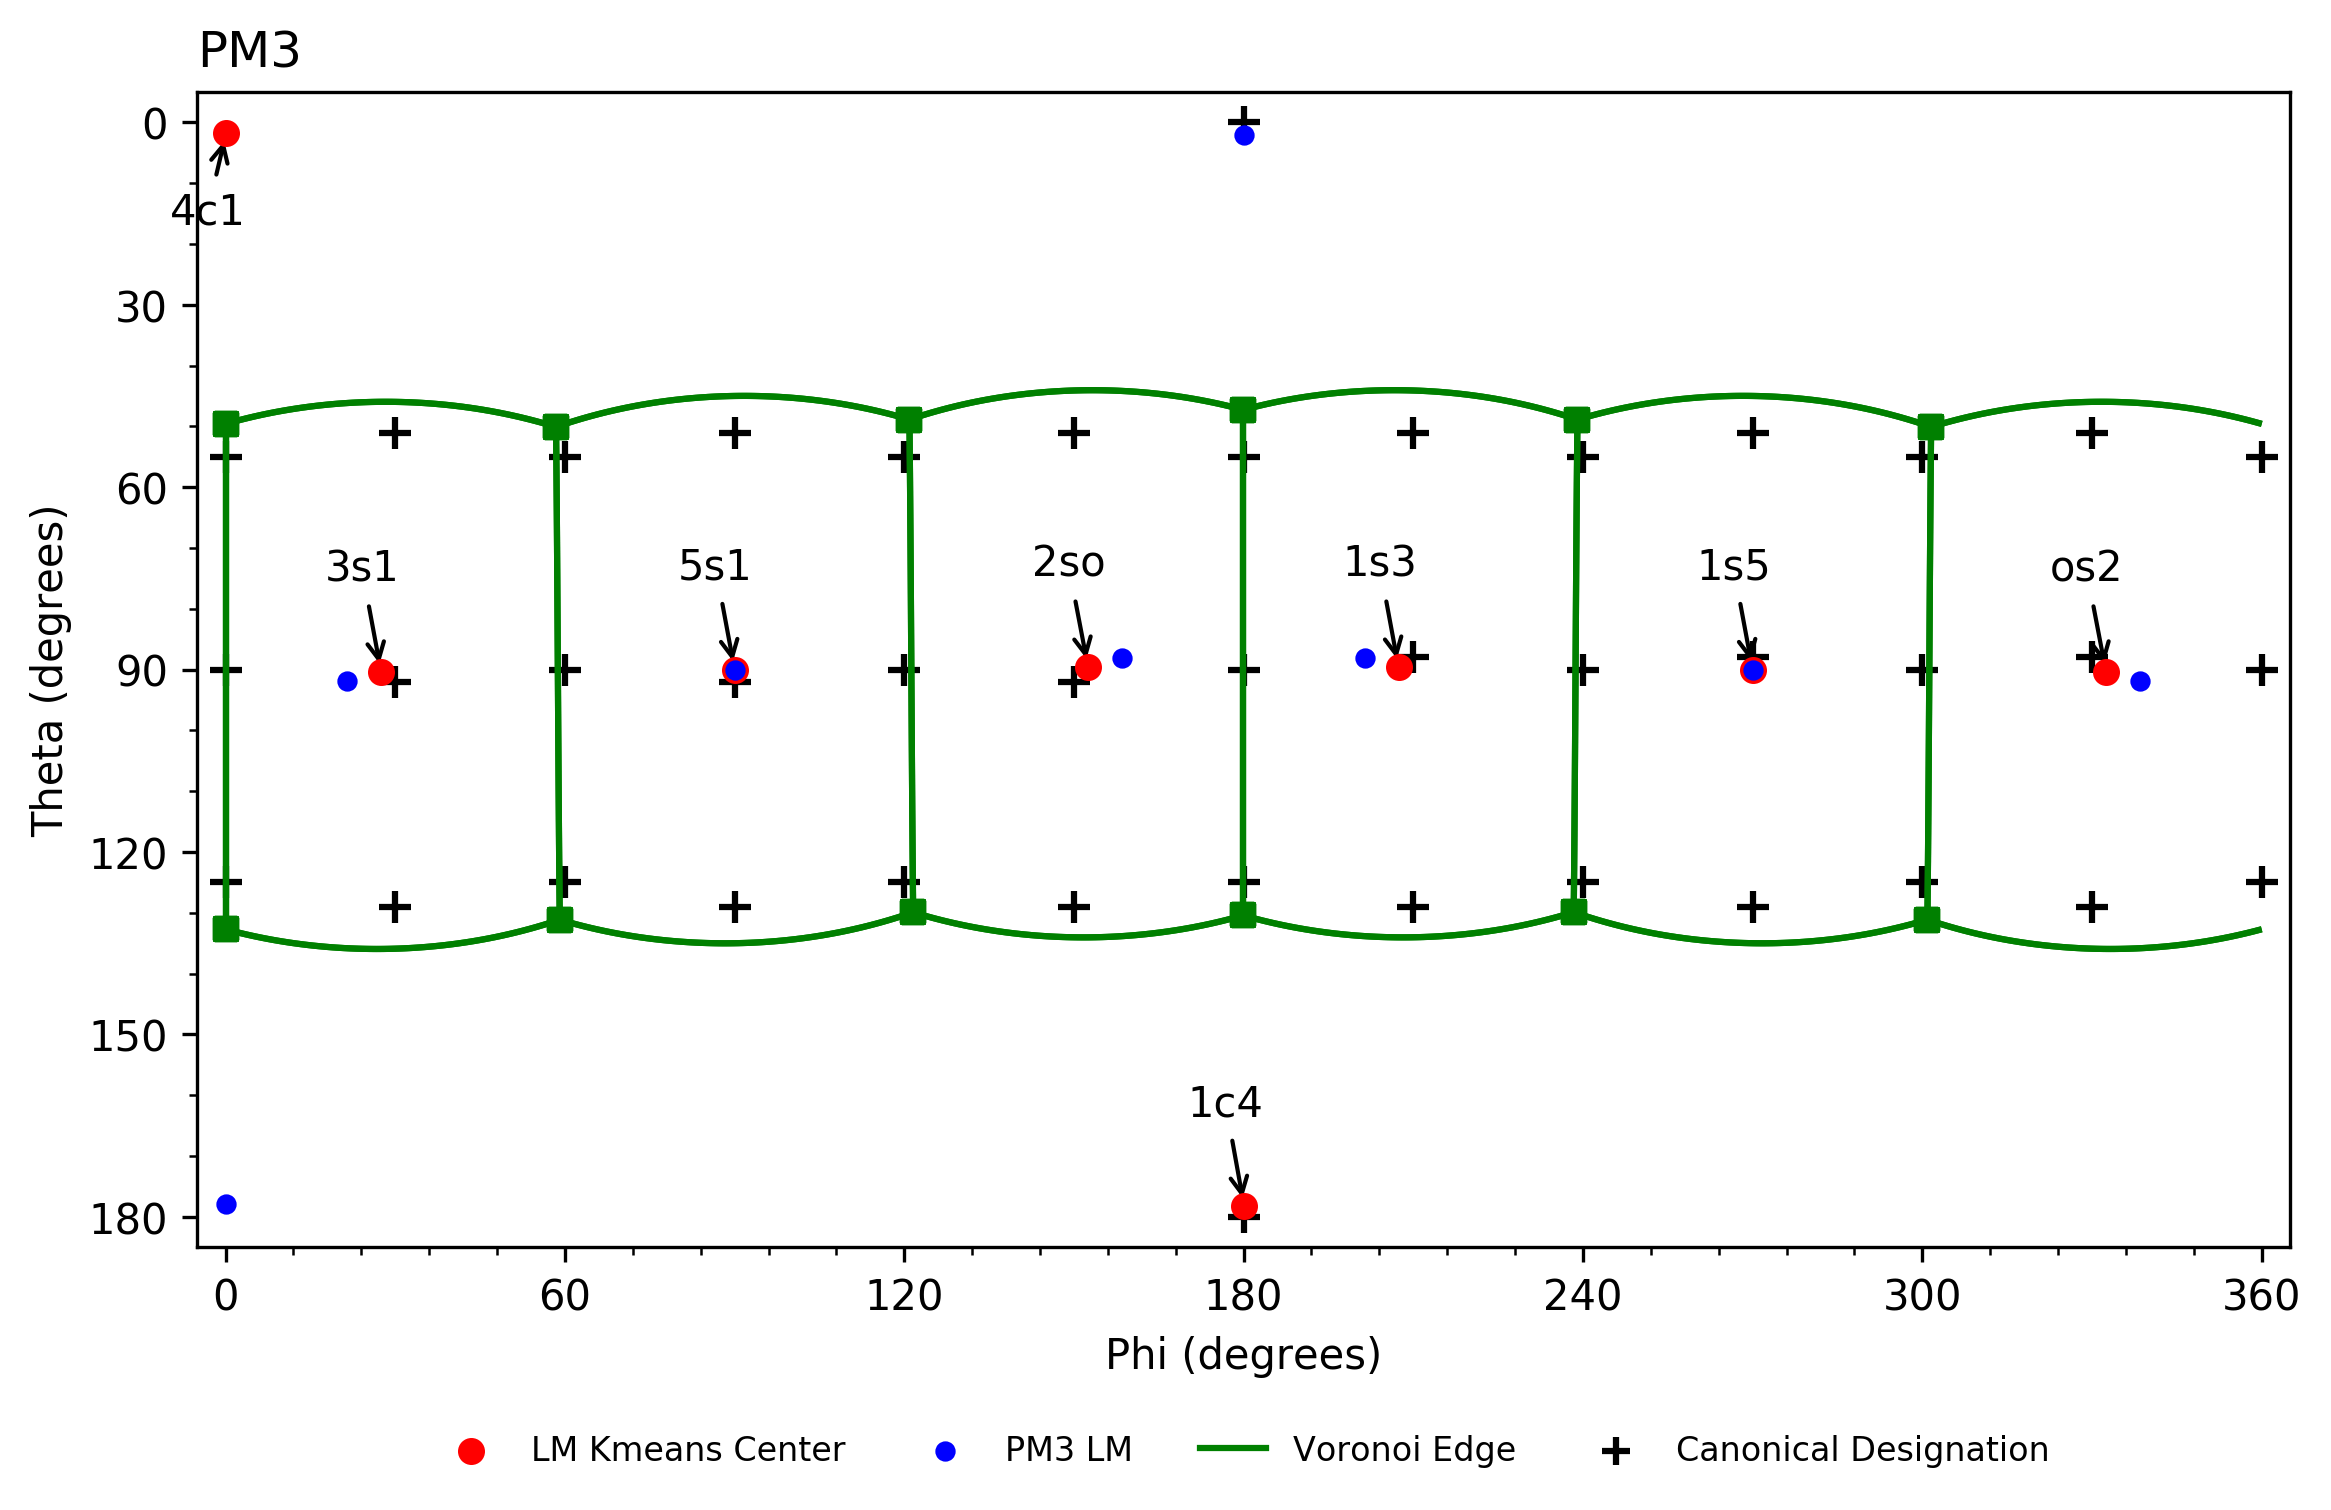
\includegraphics[width=1\textwidth,keepaspectratio]
   	{figures/oxane/overall/z_dataset-oxane-LM-PM3-all_groupings.png}
	\caption{PM3}
	\end{subfigure}
\end{figure}

\begin{figure}[H]\ContinuedFloat
	\centering
   	\begin{subfigure}[b]{0.49\textwidth}
   	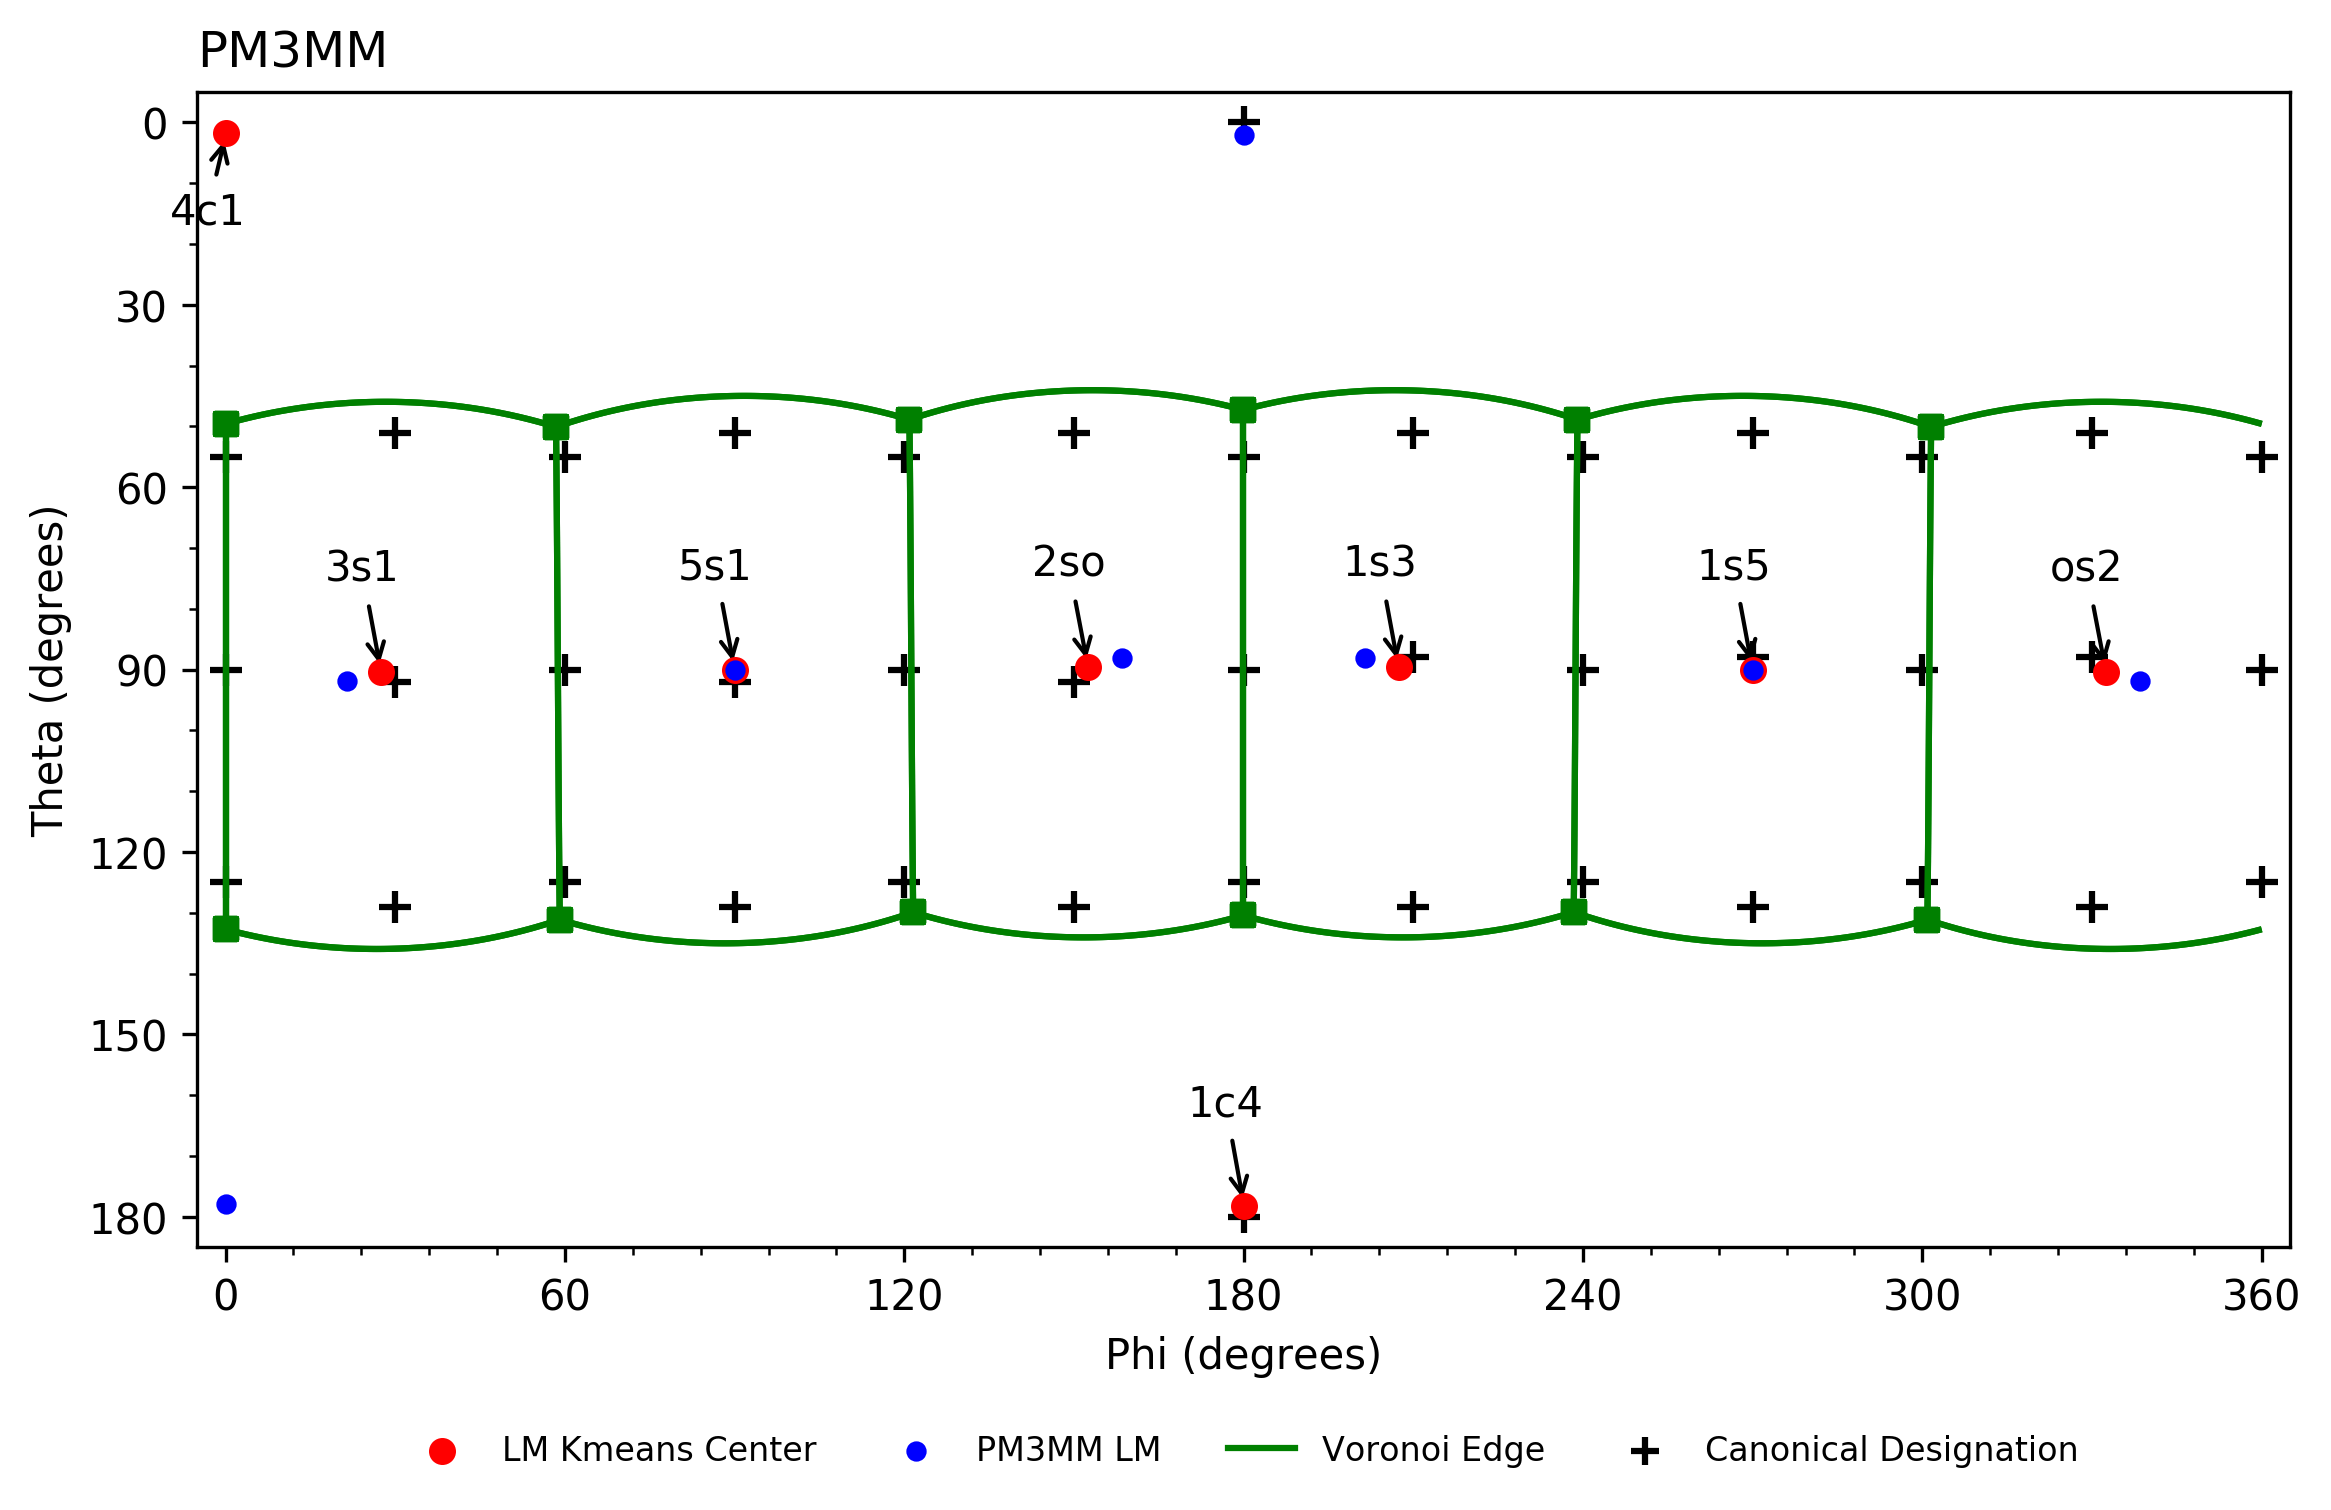
\includegraphics[width=1\textwidth,keepaspectratio]
   	{figures/oxane/overall/z_dataset-oxane-LM-PM3MM-all_groupings.png}
   	\caption{PM3MM}
	\end{subfigure}
	~
	\begin{subfigure}[b]{0.49\textwidth}
	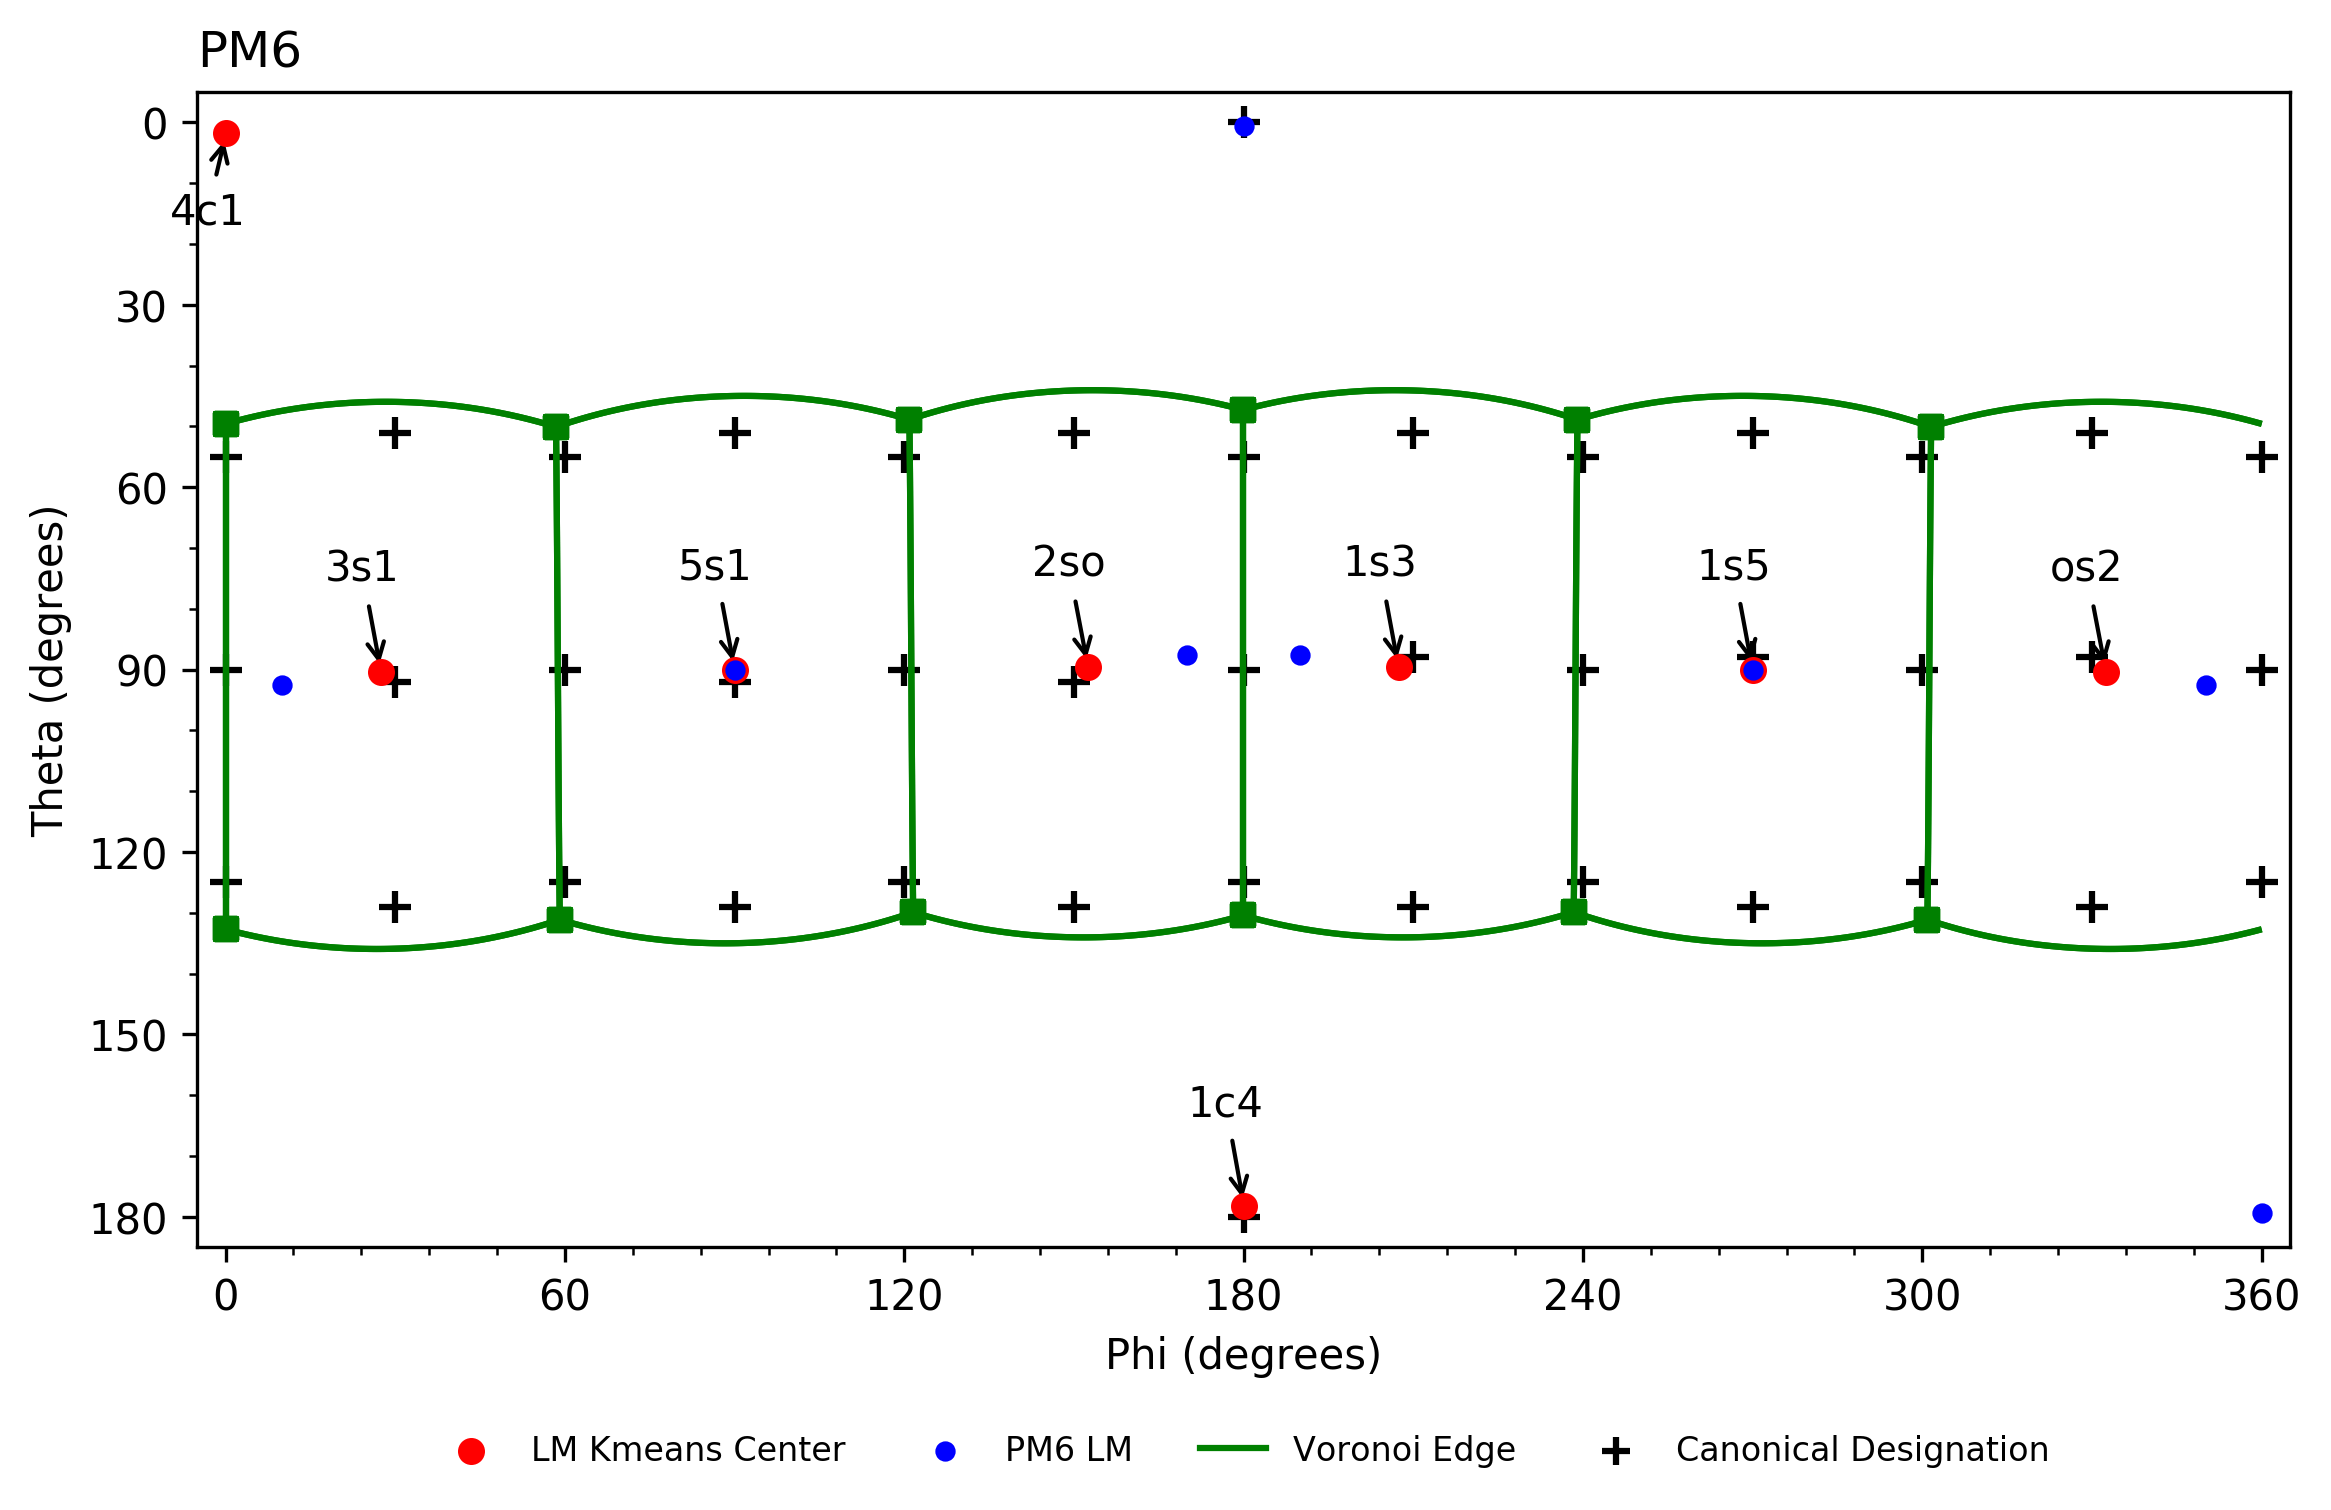
\includegraphics[width=1\textwidth,keepaspectratio]
   	{figures/oxane/overall/z_dataset-oxane-LM-PM6-all_groupings.png}
	\caption{PM6}
	\end{subfigure}
\caption{\hl{Insert Caption}}
\label{fig:oxane-ALL-LM}
\end{figure}



\subsubsection{Transition State Landscapes}
% insert the image of all of the QM methods and how the predict the different TS landscapes (show the differences) 
\begin{figure}[H]
	\centering
	\begin{subfigure}[b]{0.48\textwidth}
		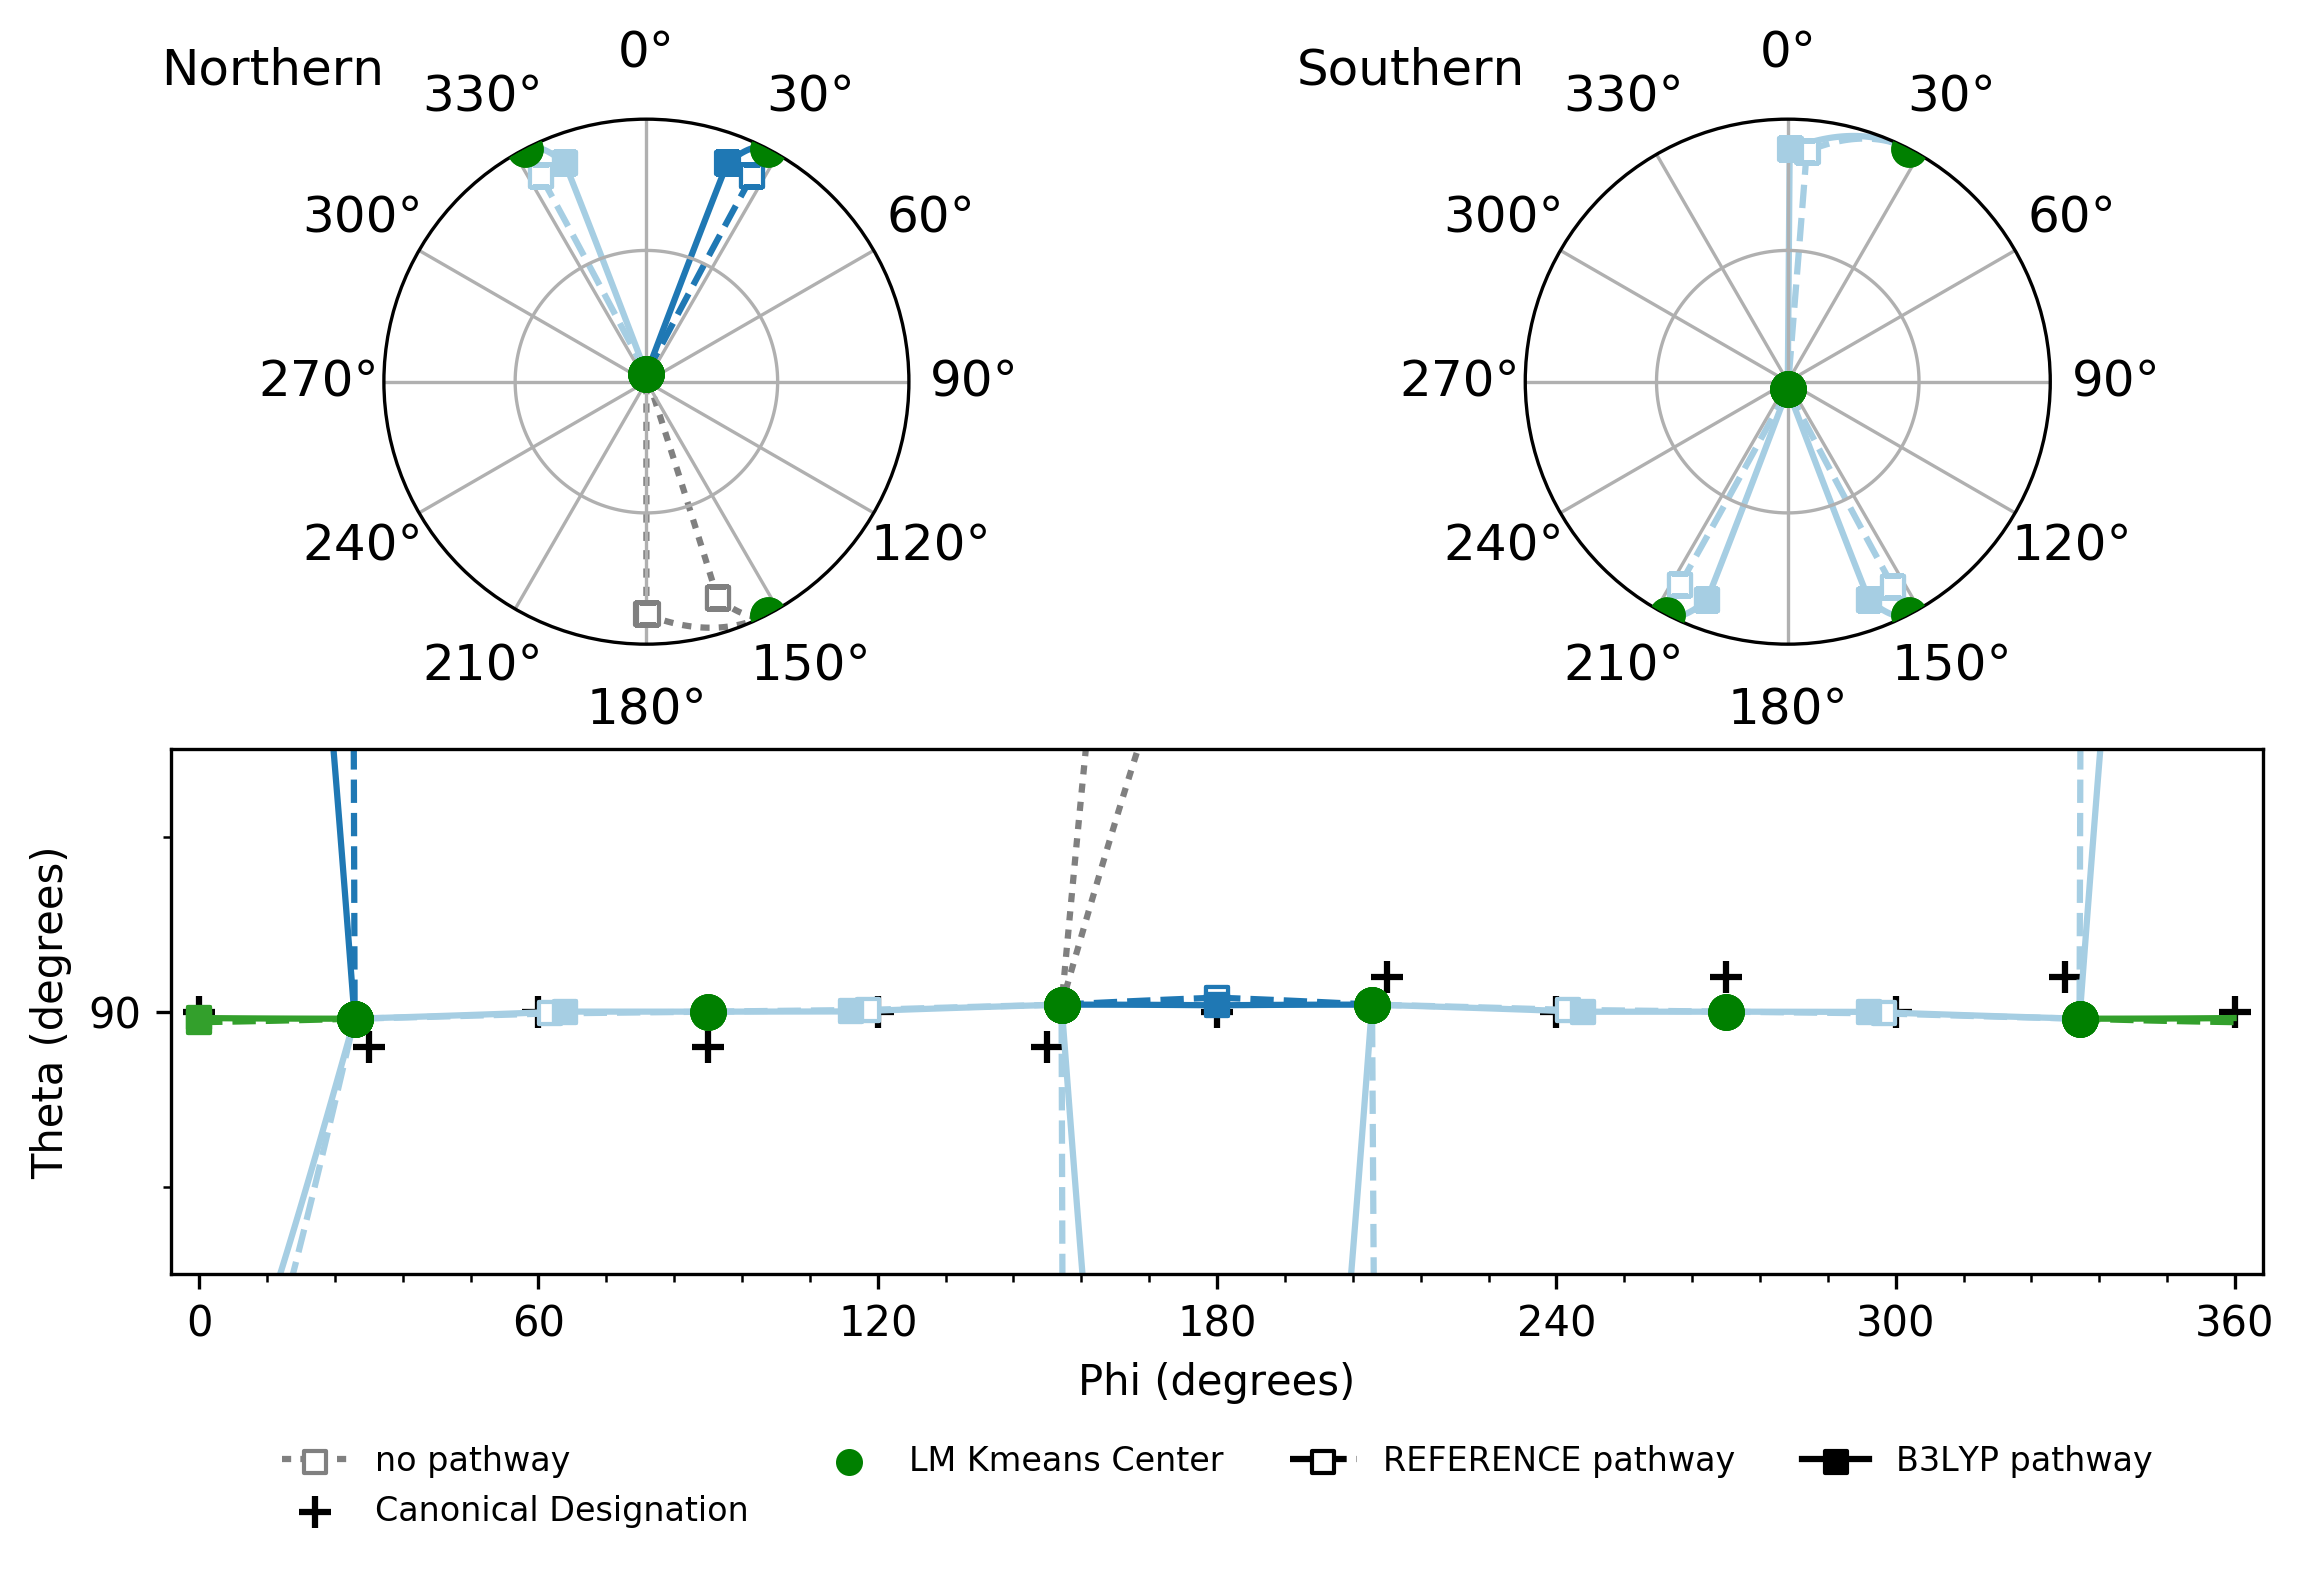
\includegraphics[width=1\textwidth,keepaspectratio]
		{figures/oxane/all_groups/z_dataset-oxane-TS--all_groups_comp-B3LYP.png}
		\caption{B3LYP/6$-$31+G(d,p)}
	\end{subfigure}
	~
	\begin{subfigure}[b]{0.48\textwidth}
		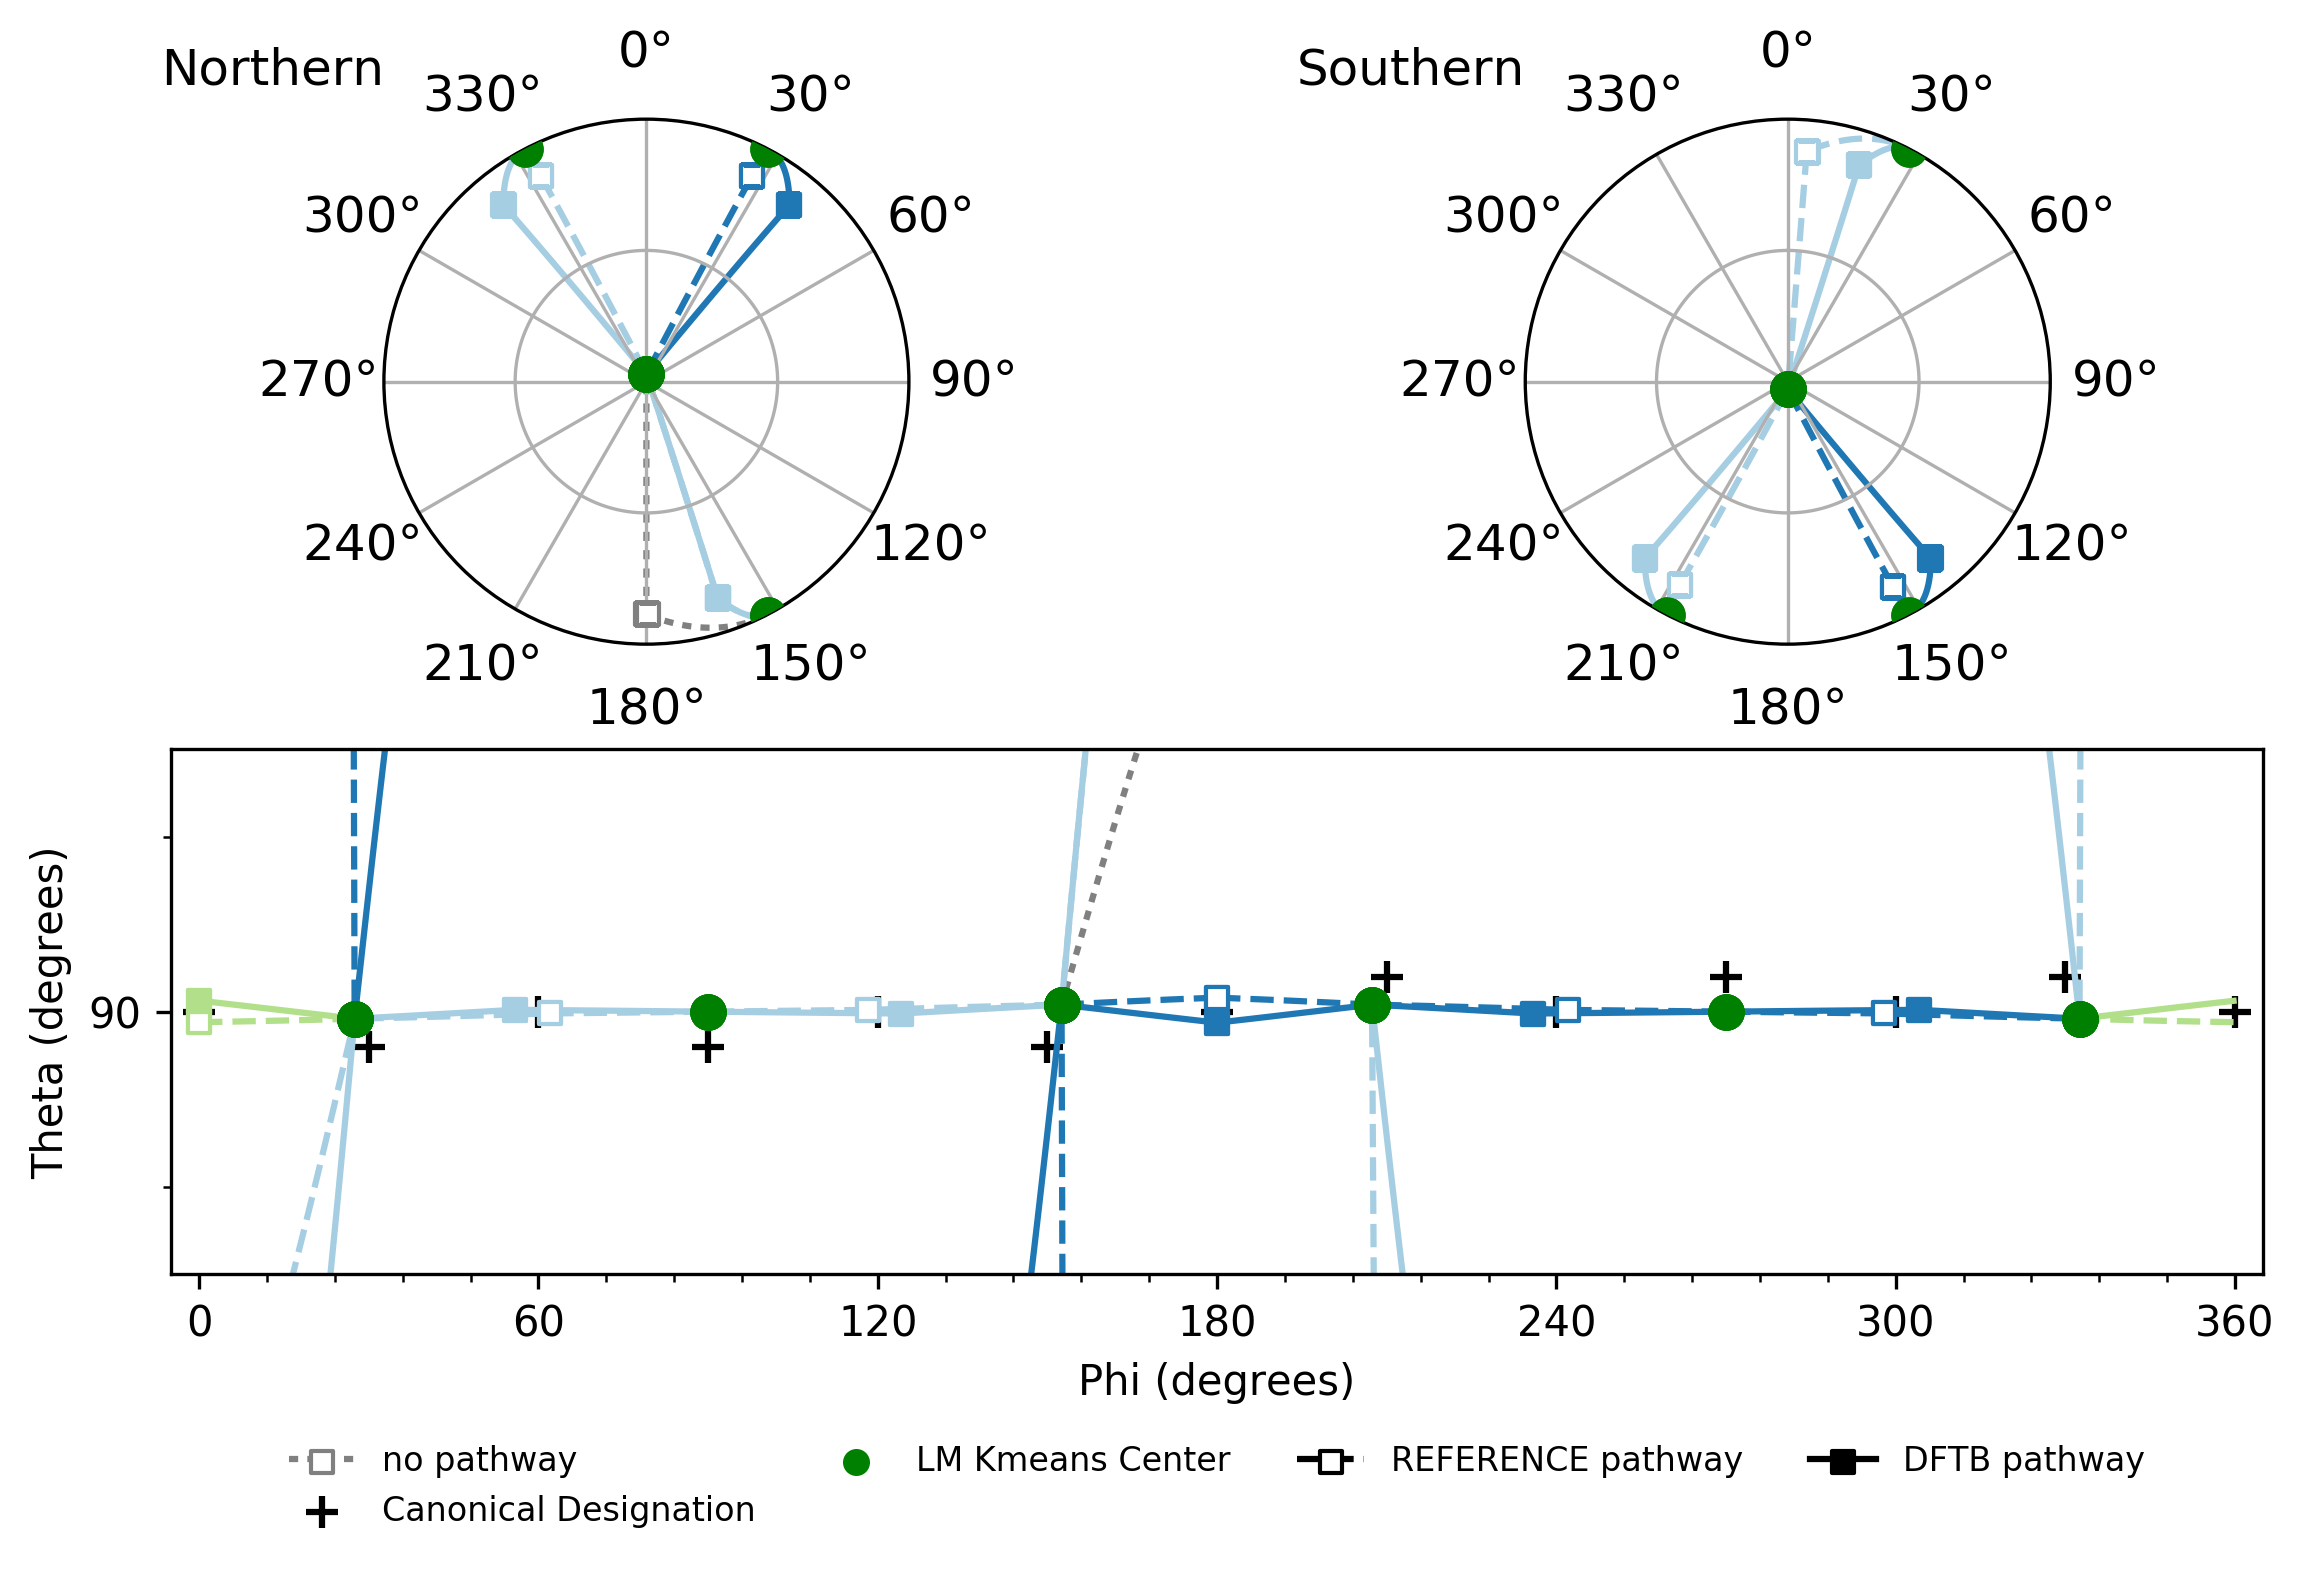
\includegraphics[width=1\textwidth,keepaspectratio]
		{figures/oxane/all_groups/z_dataset-oxane-TS--all_groups_comp-DFTB.png}
		\caption{DFTB}
	\end{subfigure}
\end{figure}

\begin{figure}[H]\ContinuedFloat
	\centering
	\begin{subfigure}[b]{0.48\textwidth}
		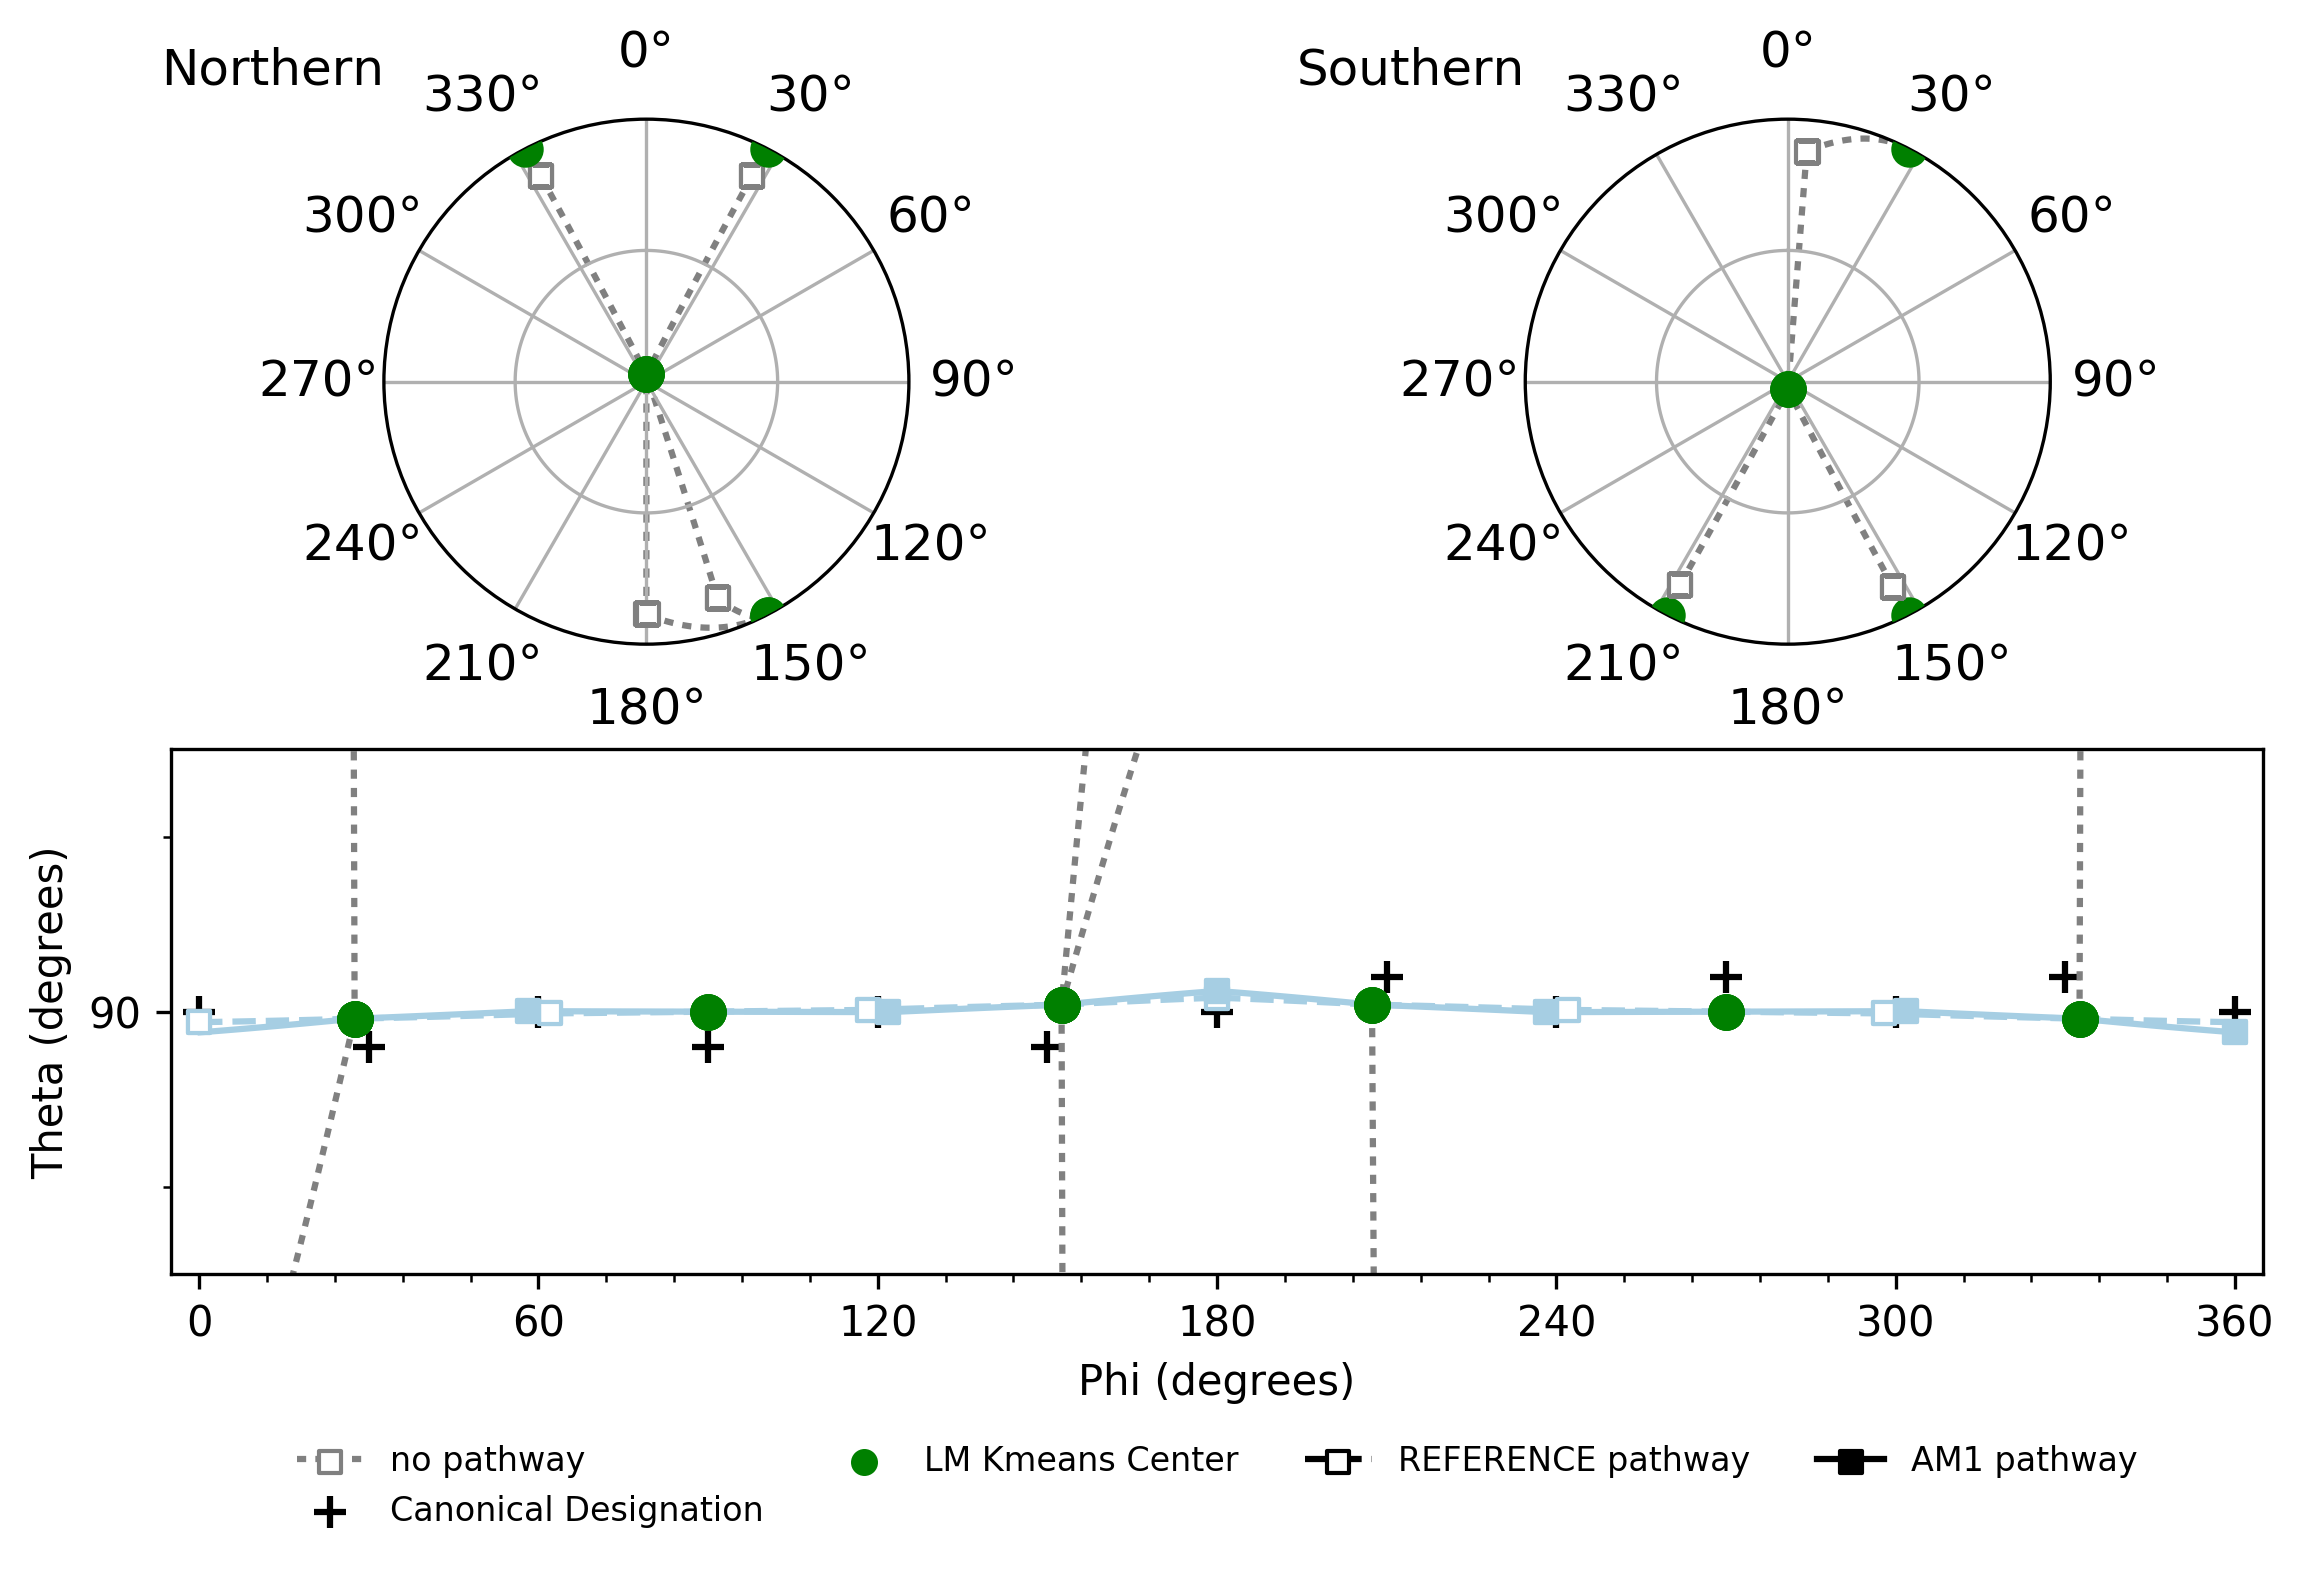
\includegraphics[width=1\textwidth,keepaspectratio]
		{figures/oxane/all_groups/z_dataset-oxane-TS--all_groups_comp-AM1.png}
		\caption{AM1}
	\end{subfigure}
	~
	\begin{subfigure}[b]{0.48\textwidth}
		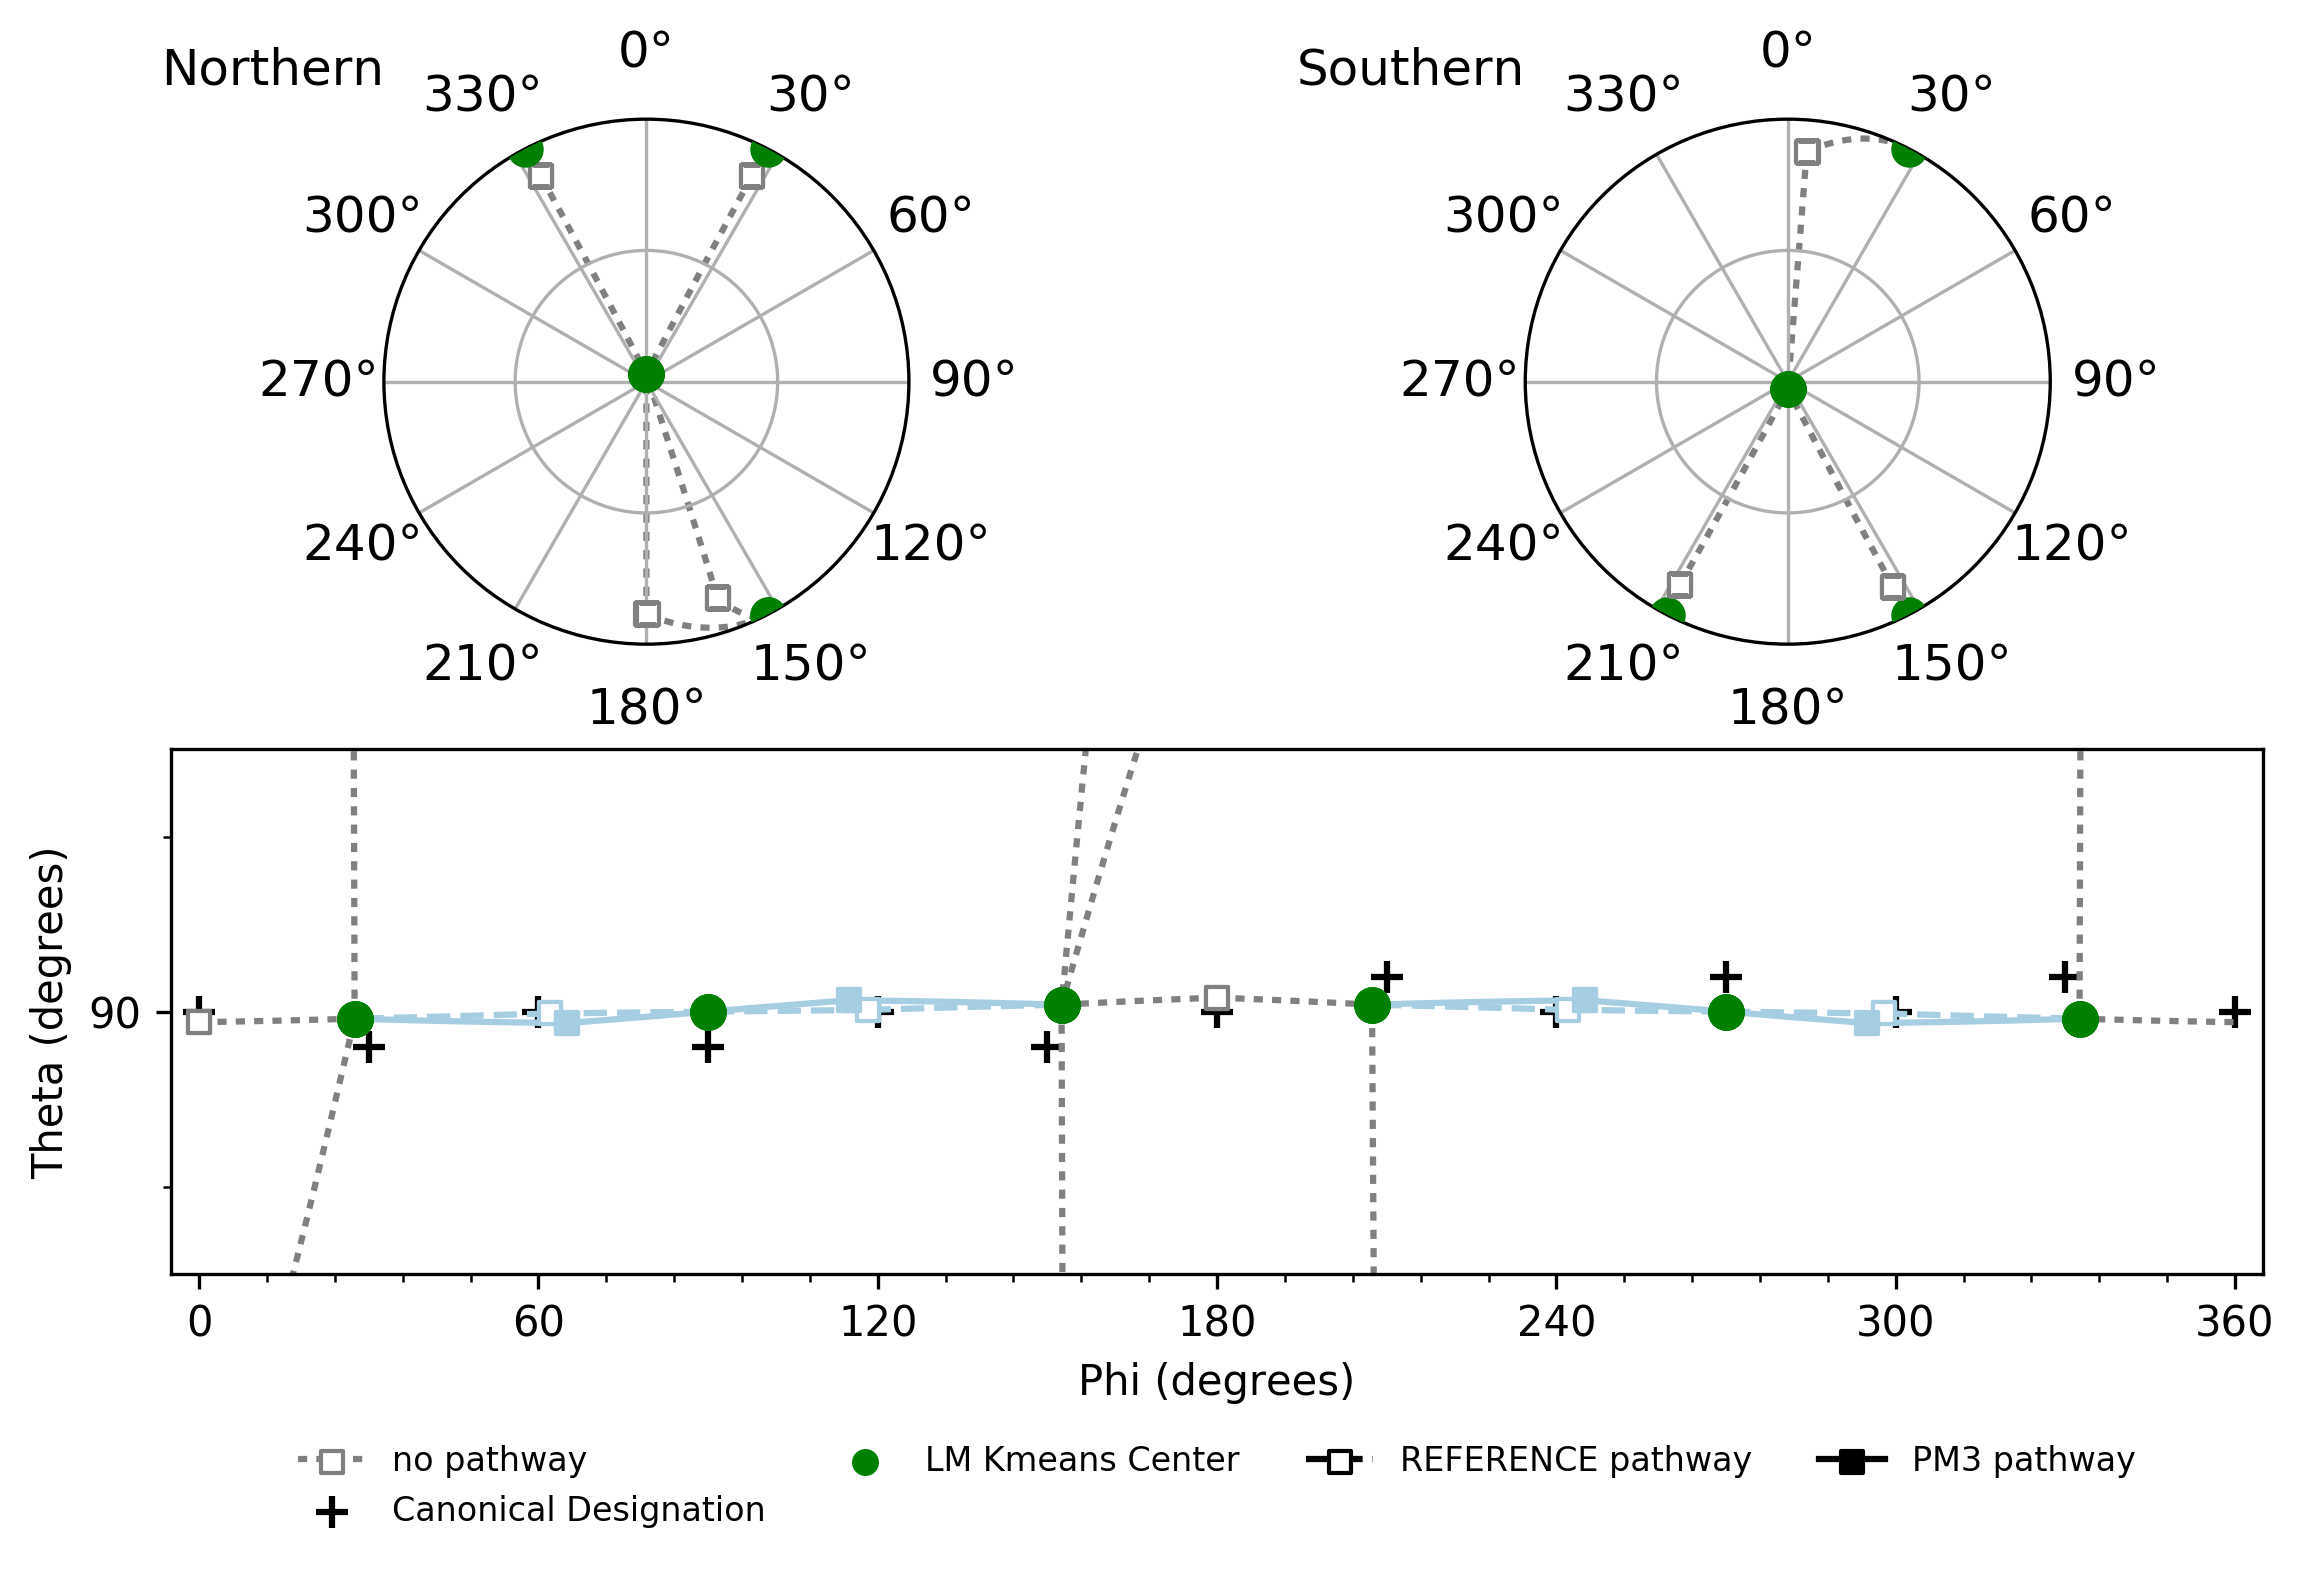
\includegraphics[width=1\textwidth,keepaspectratio]
		{figures/oxane/all_groups/z_dataset-oxane-TS--all_groups_comp-PM3.png}
		\caption{PM3}
	\end{subfigure}
\end{figure}

\begin{figure}[H]\ContinuedFloat
	\centering
	\begin{subfigure}[b]{0.48\textwidth}
		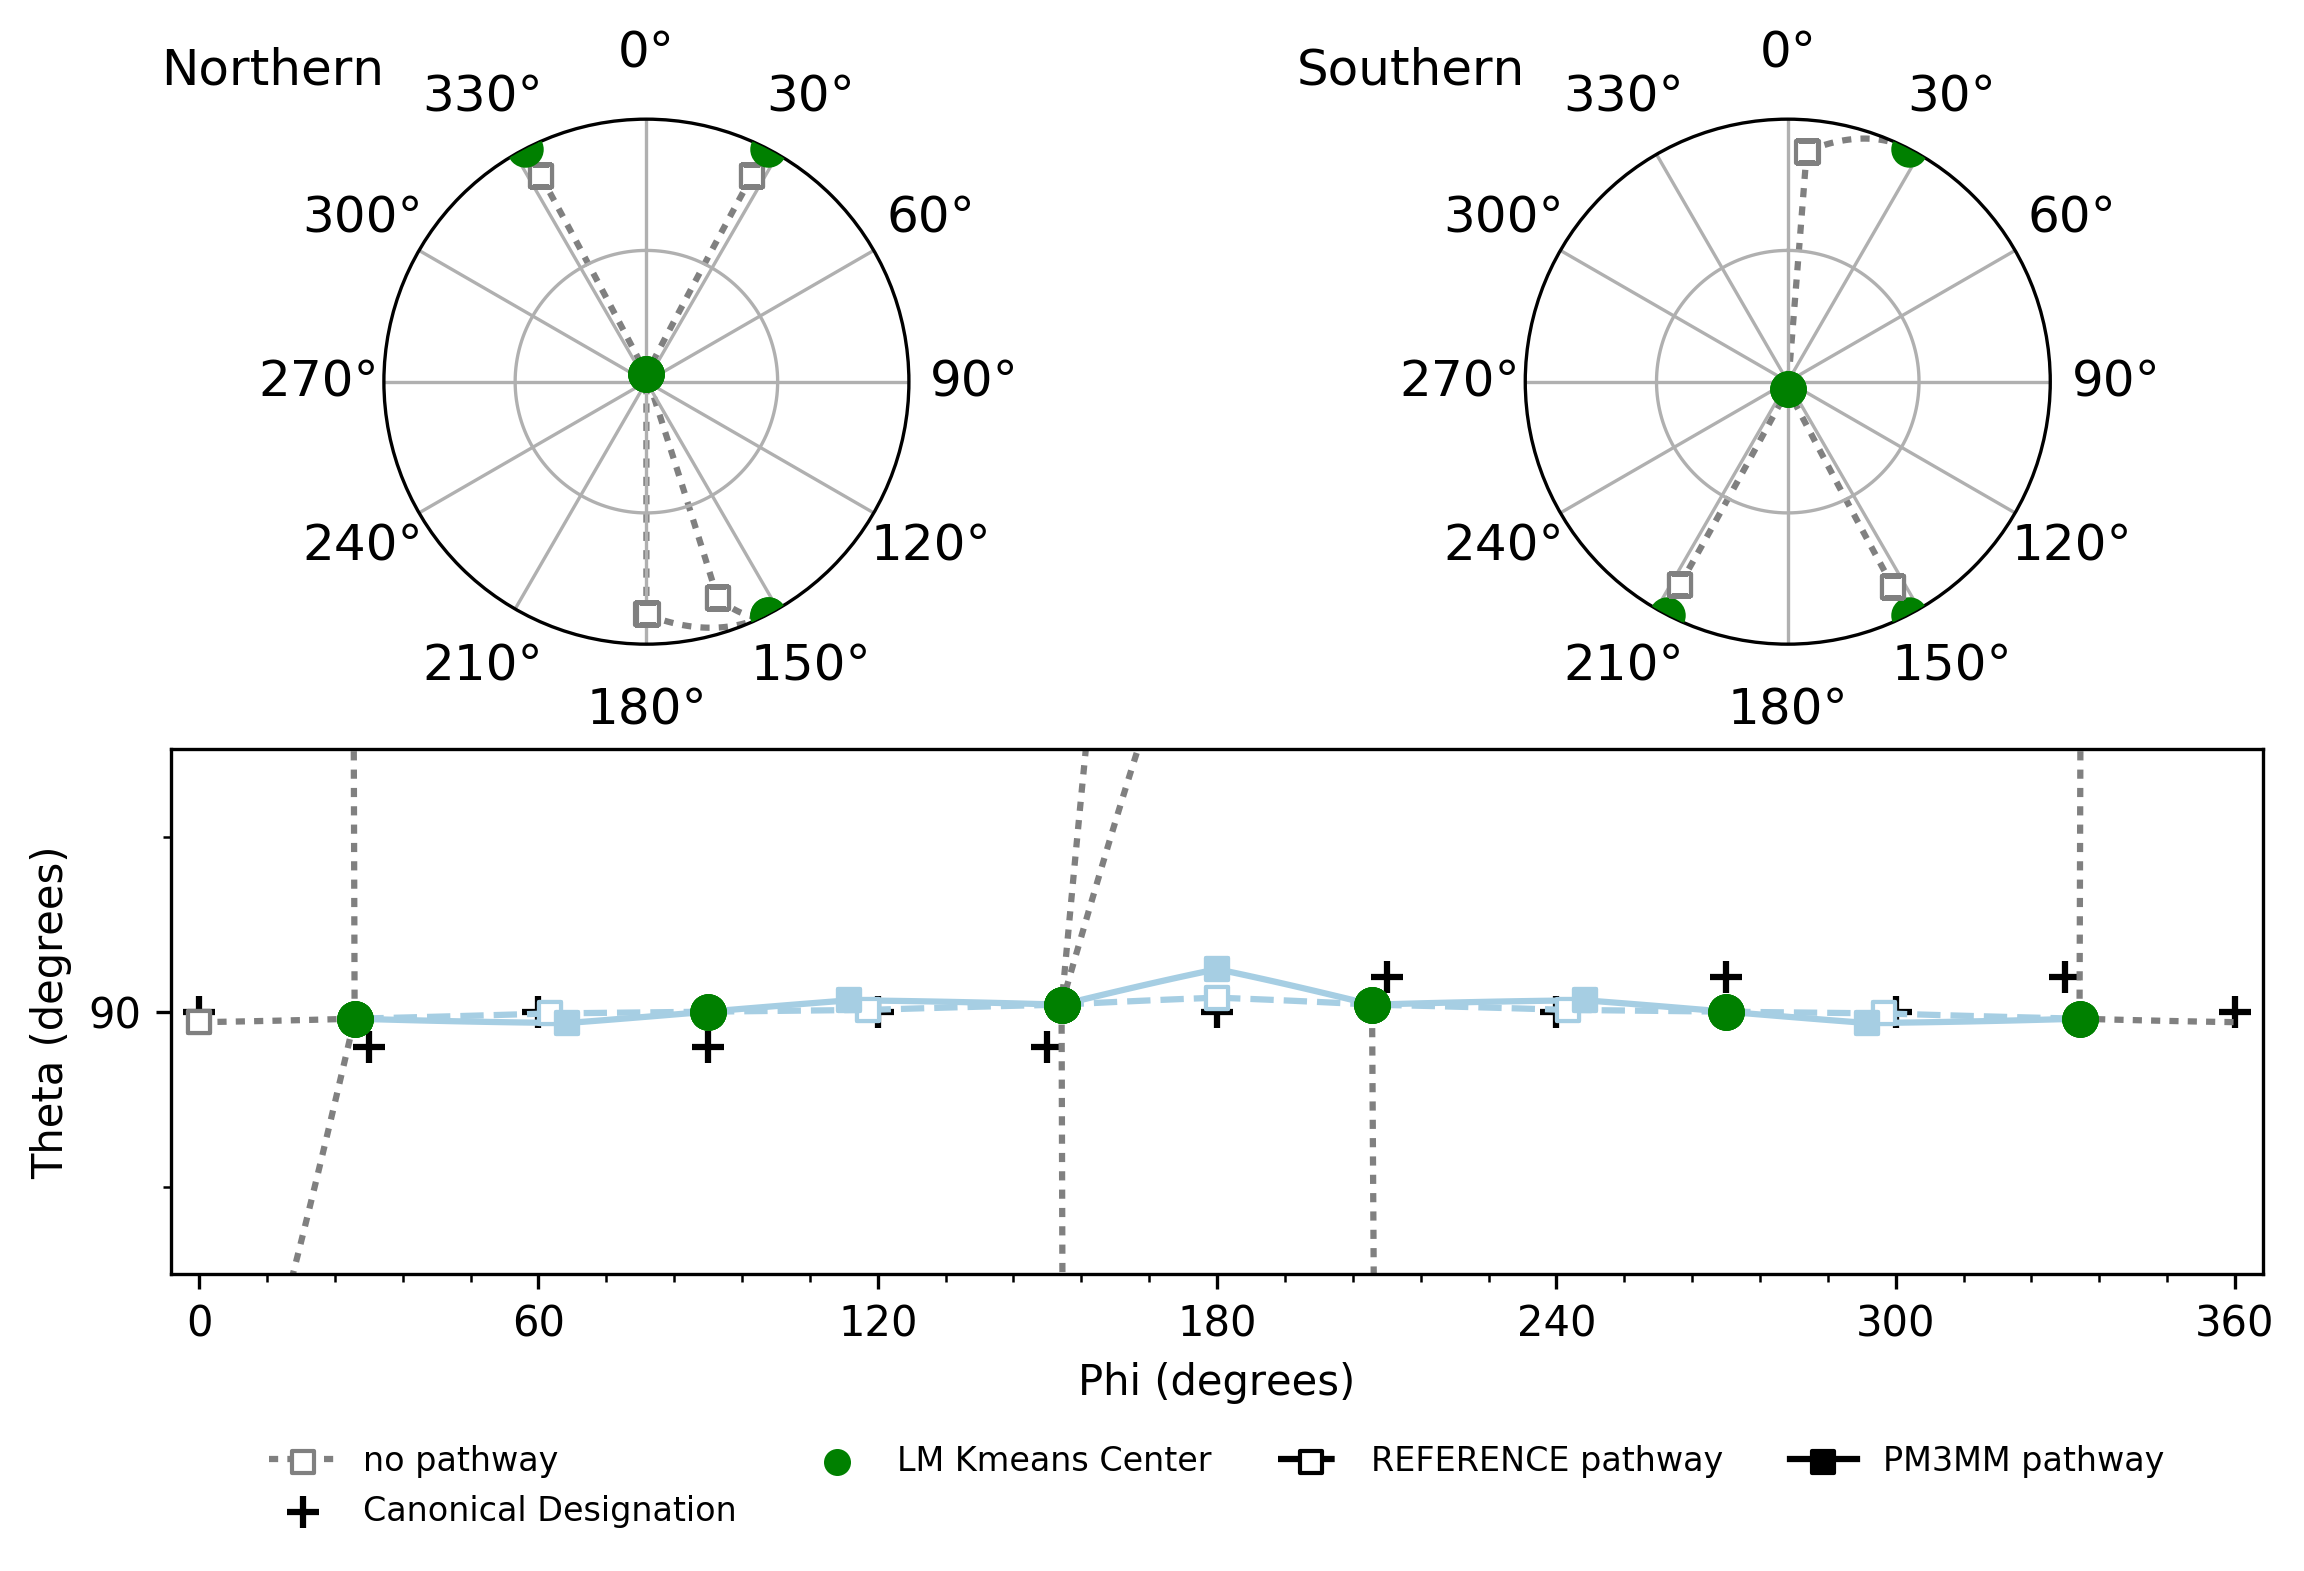
\includegraphics[width=1\textwidth,keepaspectratio]
		{figures/oxane/all_groups/z_dataset-oxane-TS--all_groups_comp-PM3MM.png}
		\caption{PM3MM}
	\end{subfigure}
	~
	\begin{subfigure}[b]{0.48\textwidth}
		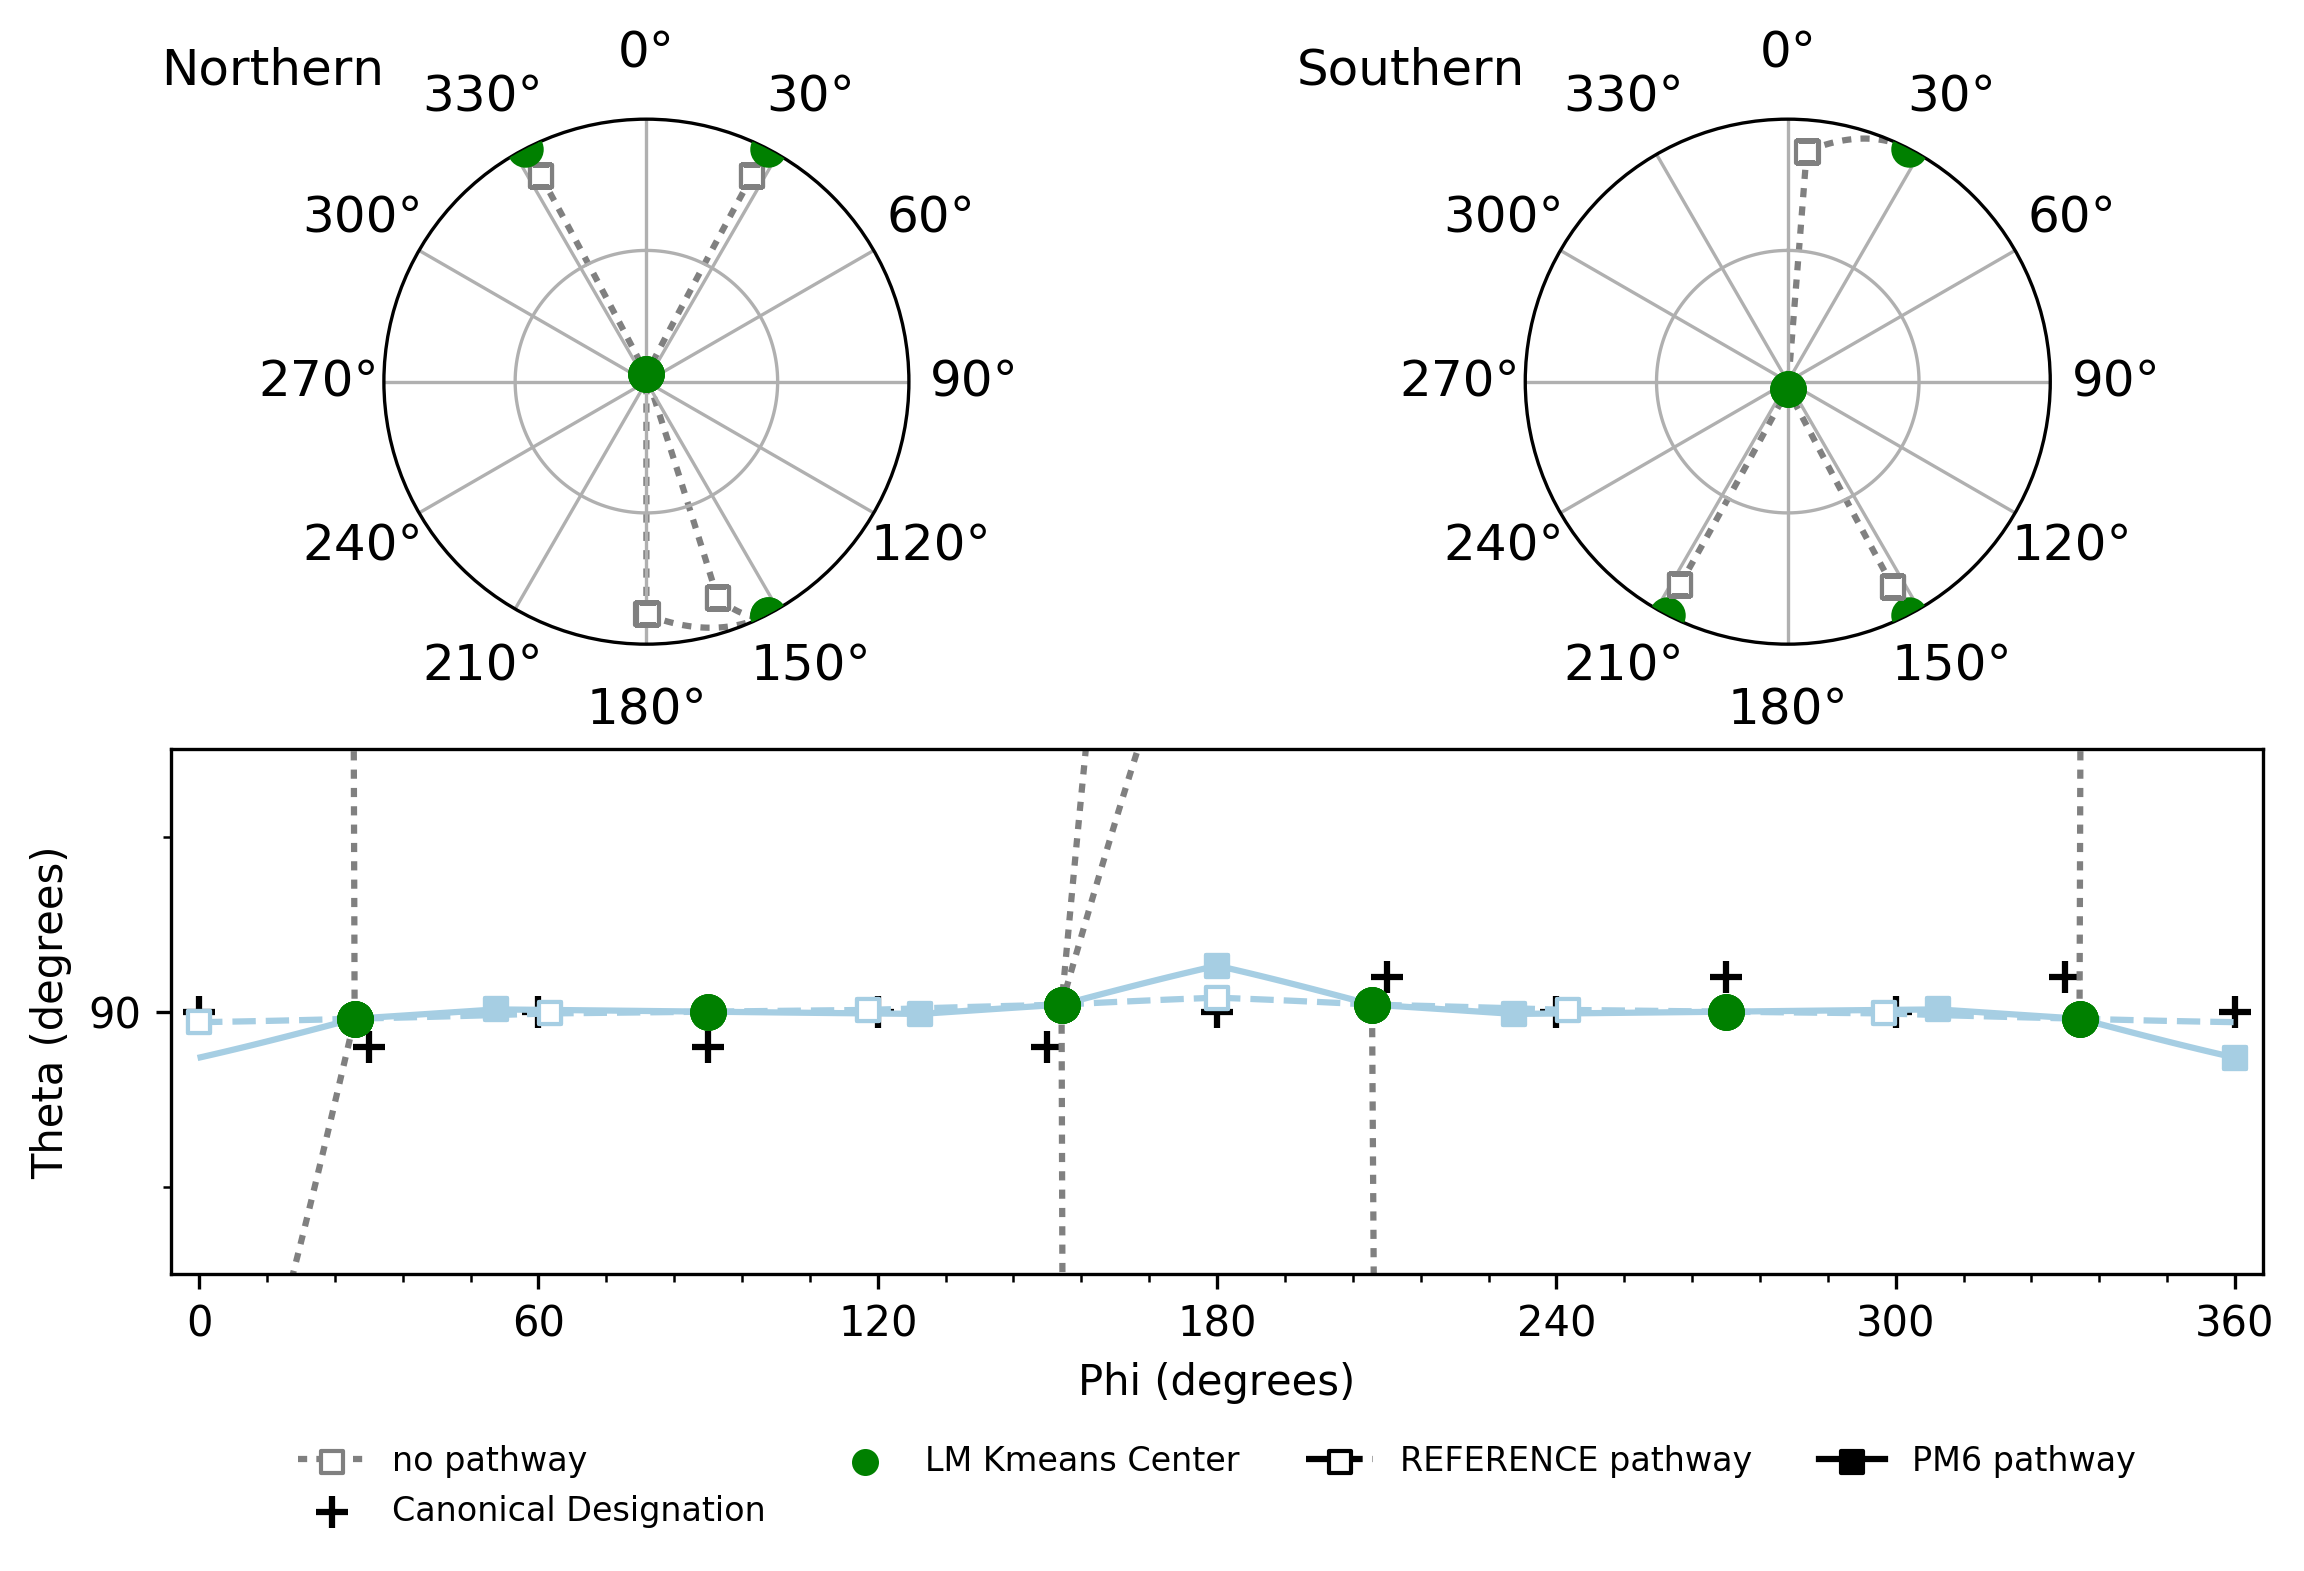
\includegraphics[width=1\textwidth,keepaspectratio]
		{figures/oxane/all_groups/z_dataset-oxane-TS--all_groups_comp-PM6.png}
		\caption{PM6}
	\end{subfigure}
	\caption{\hl{Insert Caption}}
	\label{fig:oxane-ALL-LM}
\end{figure}

\subsubsection{WRMSD Table}

\begin{figure}[H]
	\centering
	\begin{subfigure}[b]{1\textwidth}
		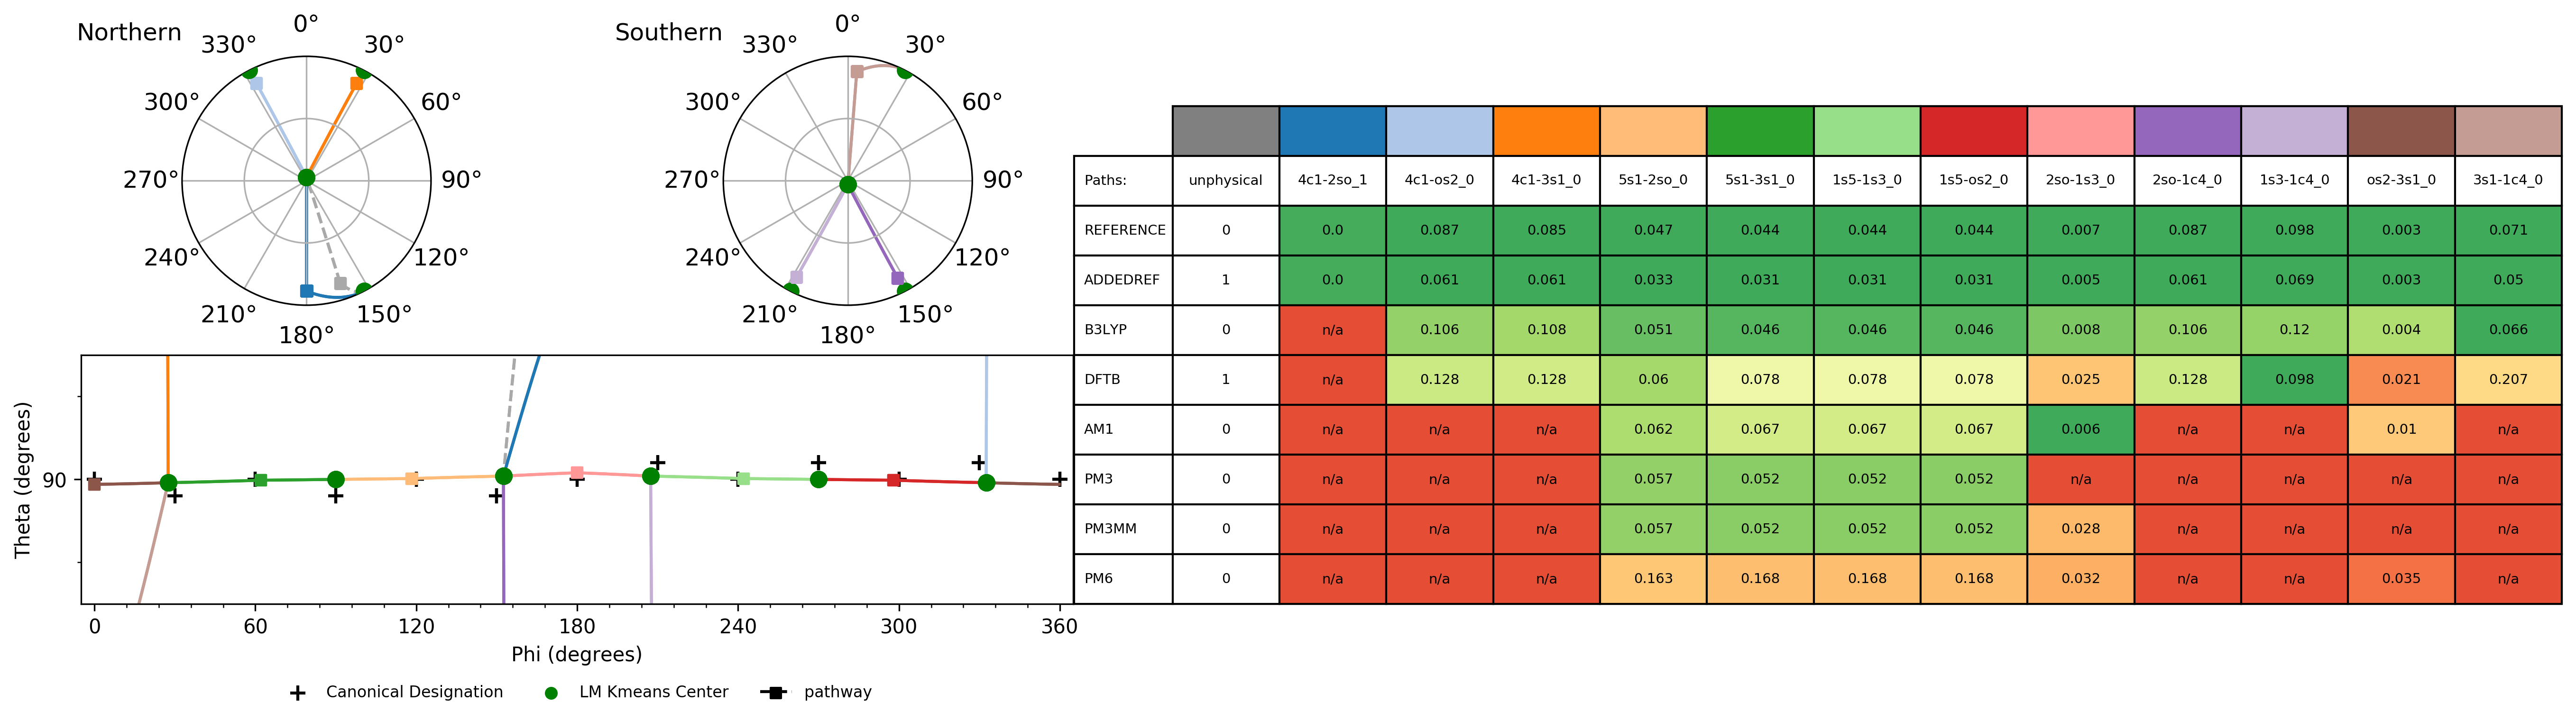
\includegraphics[width=1\textwidth,keepaspectratio]
		{figures/oxane/comp_tables/z_dataset-oxane-TS-all-groups-arc_group_WRMSD-table.png}
		\caption{Comparison via arclength}
	\end{subfigure}

	\begin{subfigure}[b]{1\textwidth}
		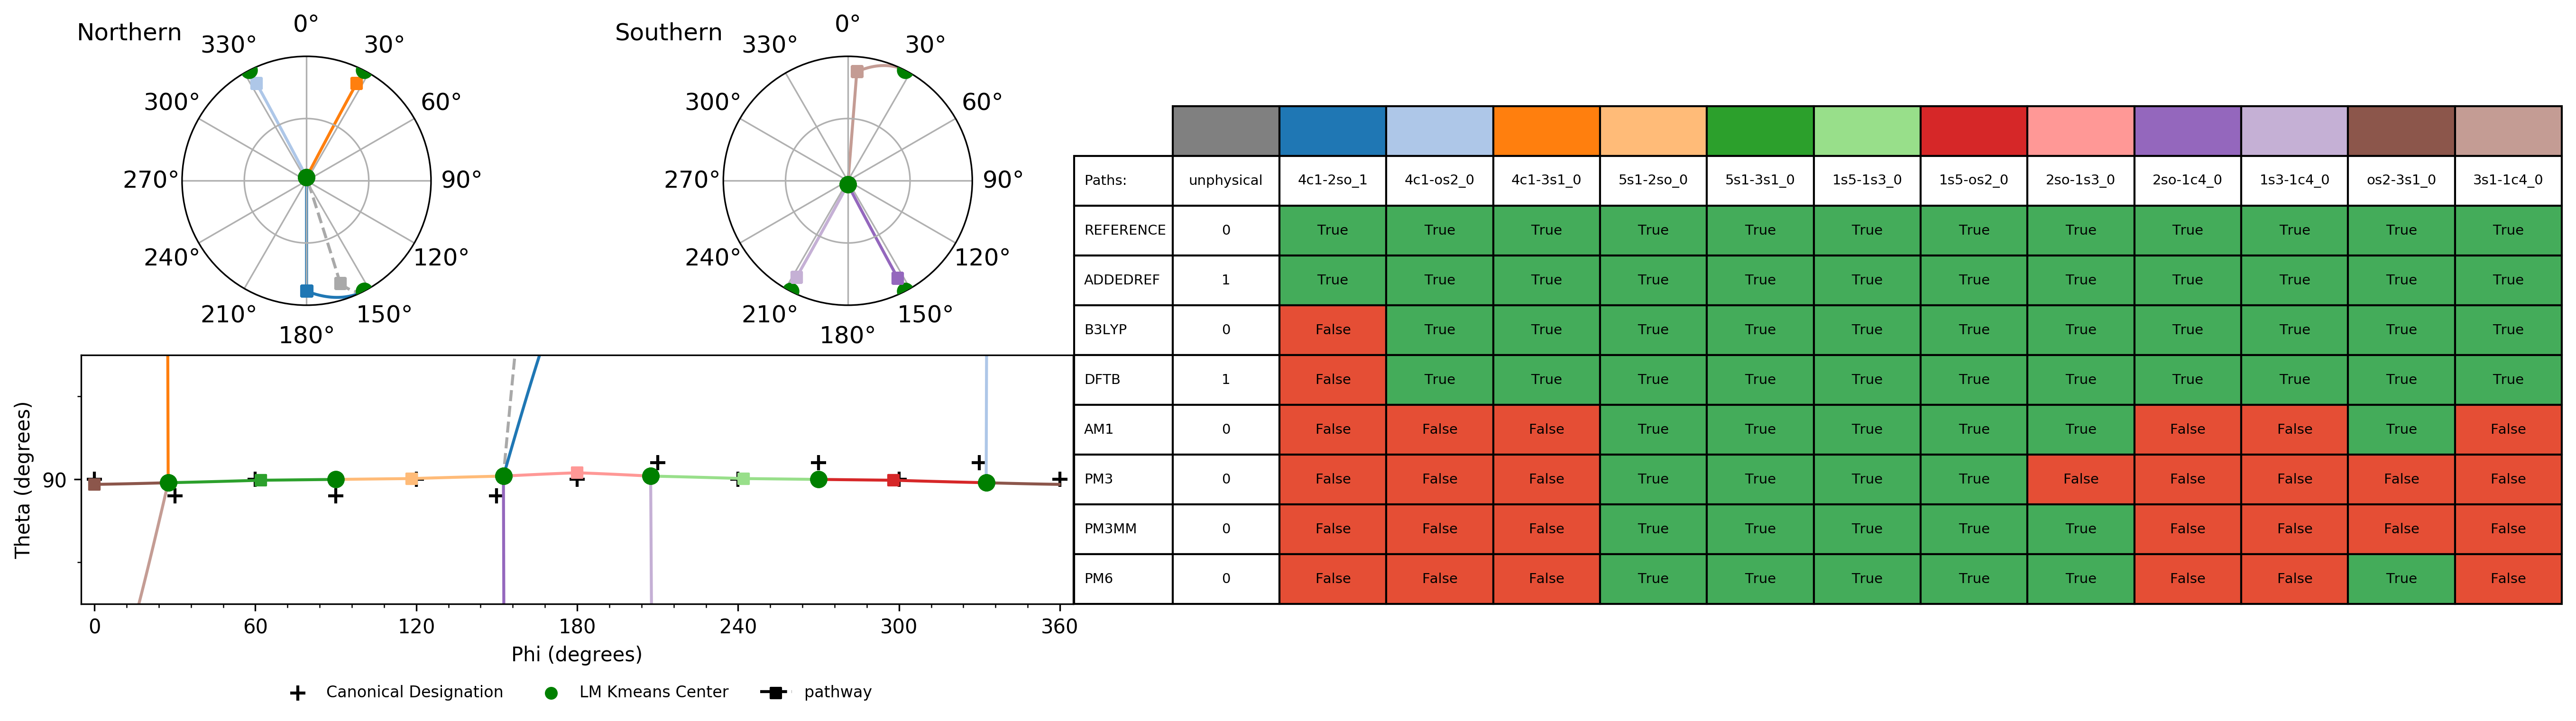
\includegraphics[width=1\textwidth,keepaspectratio]
		{figures/oxane/comp_tables/z_dataset-oxane-TS-all-groups-arc_comp-table.png}
		\caption{Binary representation}
	\end{subfigure}
\caption{\hl{Insert Caption}}
\label{fig:oxane-ALL-LM}
\end{figure}

\subsubsection{Relative Gibbs Free Energy Comparison Table}

\begin{figure}[H]
	\centering
	\begin{subfigure}[b]{1\textwidth}
		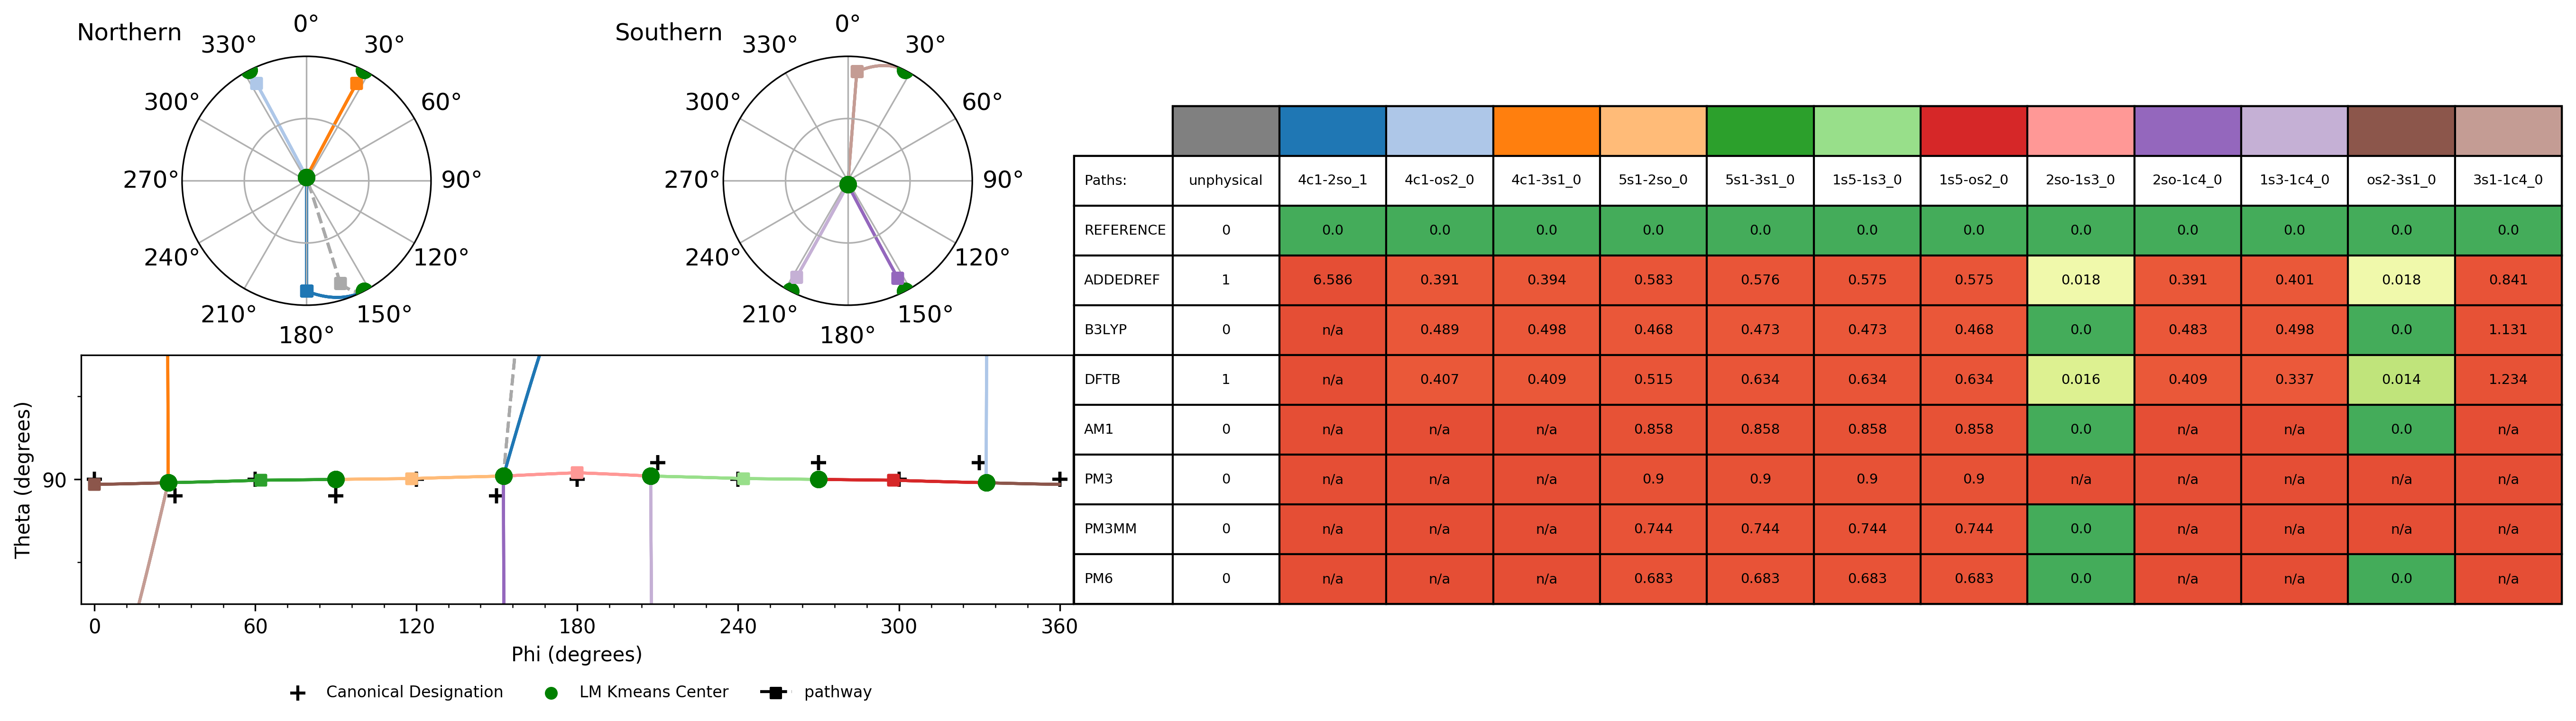
\includegraphics[width=1\textwidth,keepaspectratio]
		{figures/oxane/comp_tables/z_dataset-oxane-TS-all-groups-gibbs_group_WRMSD-table.png}
		\caption{Comparison via gibbs free energy}
	\end{subfigure}
	
	\begin{subfigure}[b]{1\textwidth}
		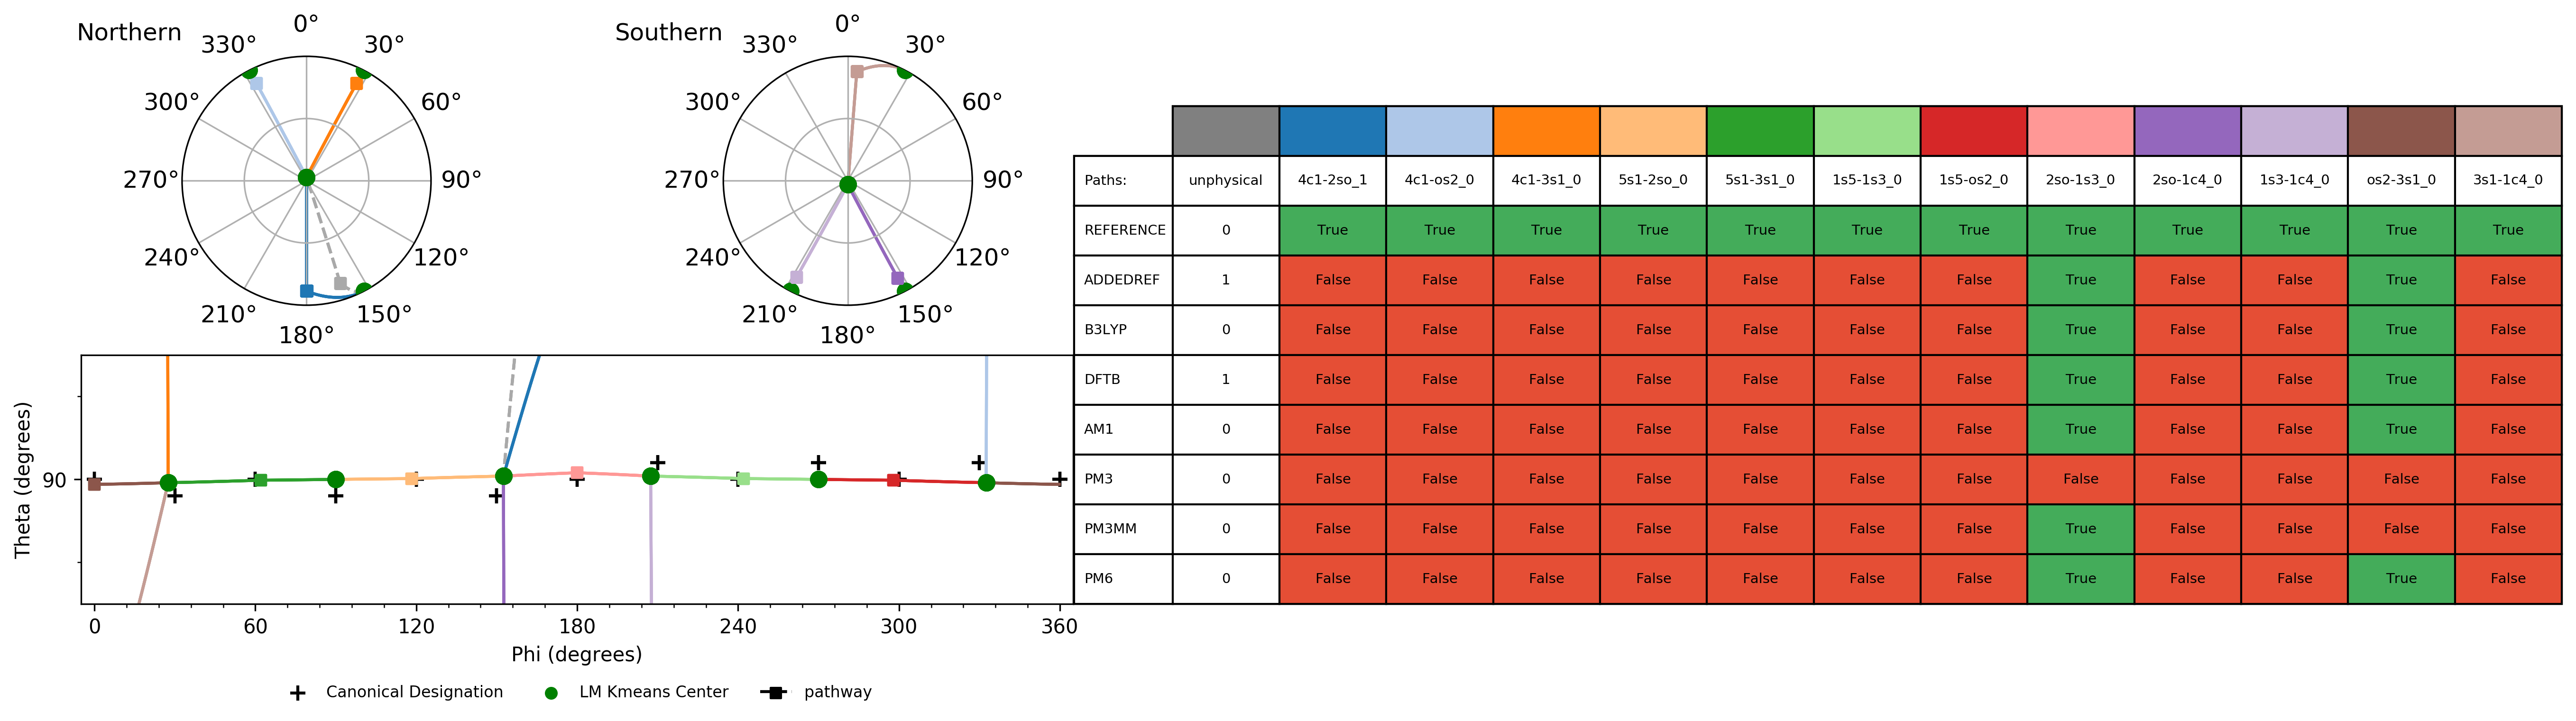
\includegraphics[width=1\textwidth,keepaspectratio]
		{figures/oxane/comp_tables/z_dataset-oxane-TS-all-groups-gibbs_comp-table.png}
		\caption{Binary representation}
	\end{subfigure}

	\begin{subfigure}[b]{0.3\textwidth}
		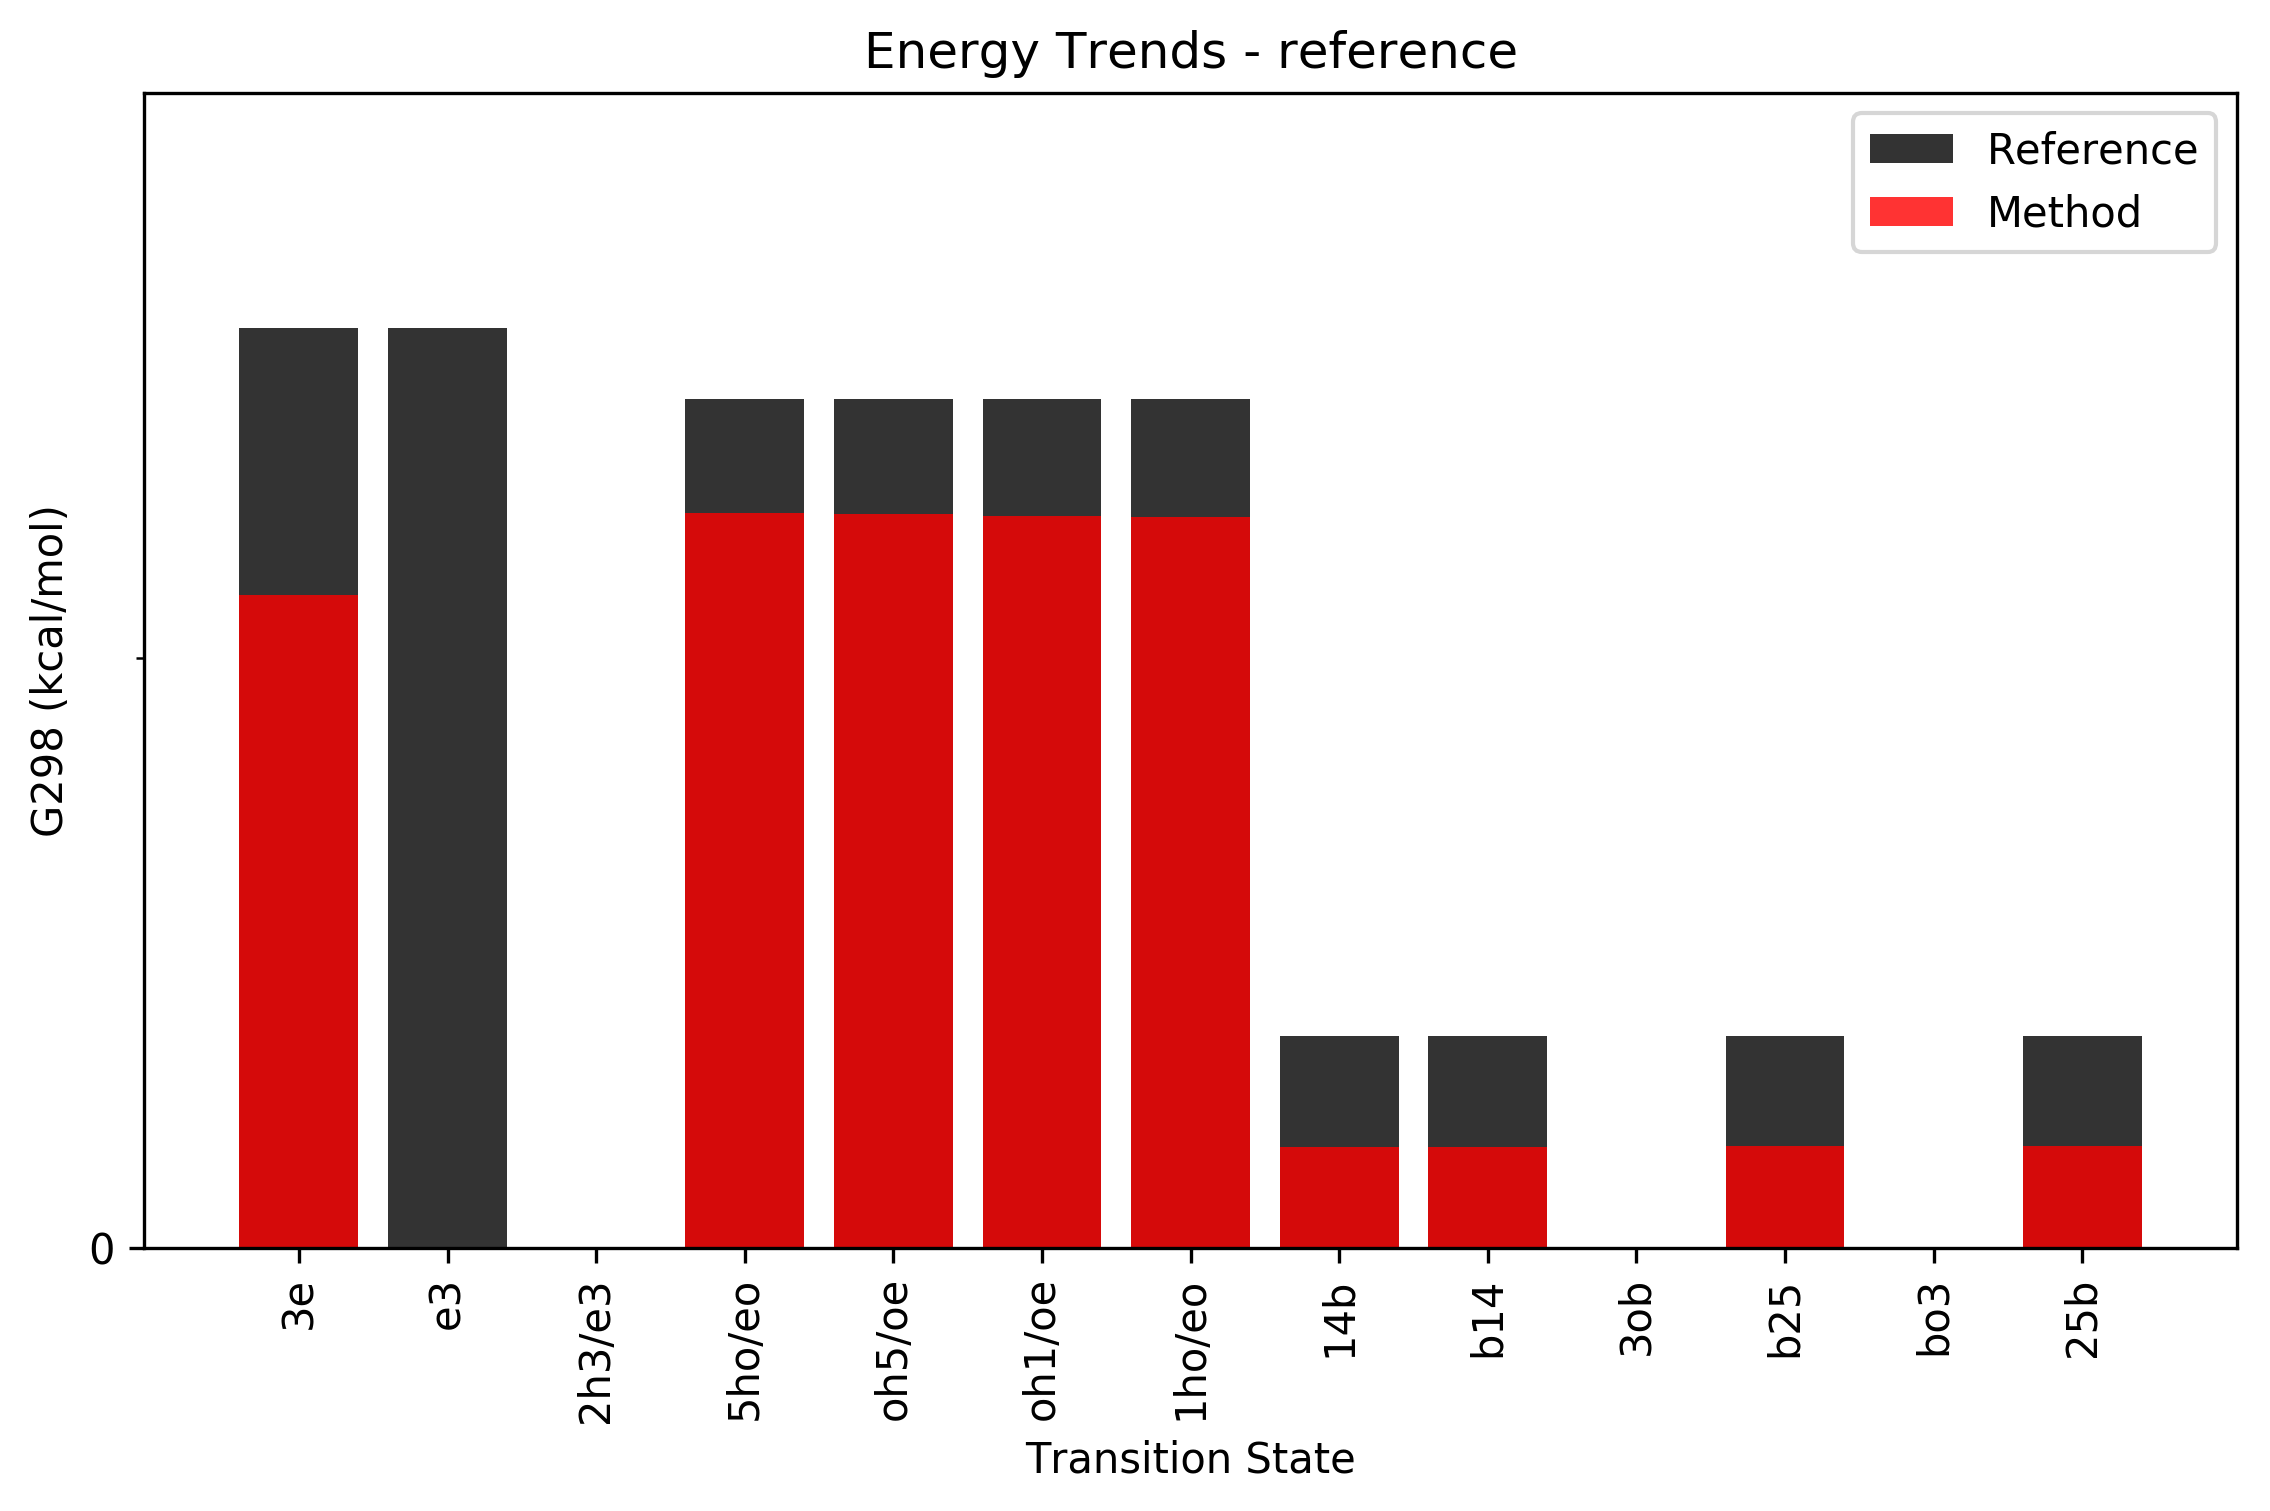
\includegraphics[width=1\textwidth,keepaspectratio]
		{figures/oxane/comp_tables/oxane-diff-trend-b3lyp.png}
		\caption{B3LYP}
	\end{subfigure}
	~
	\begin{subfigure}[b]{0.3\textwidth}
		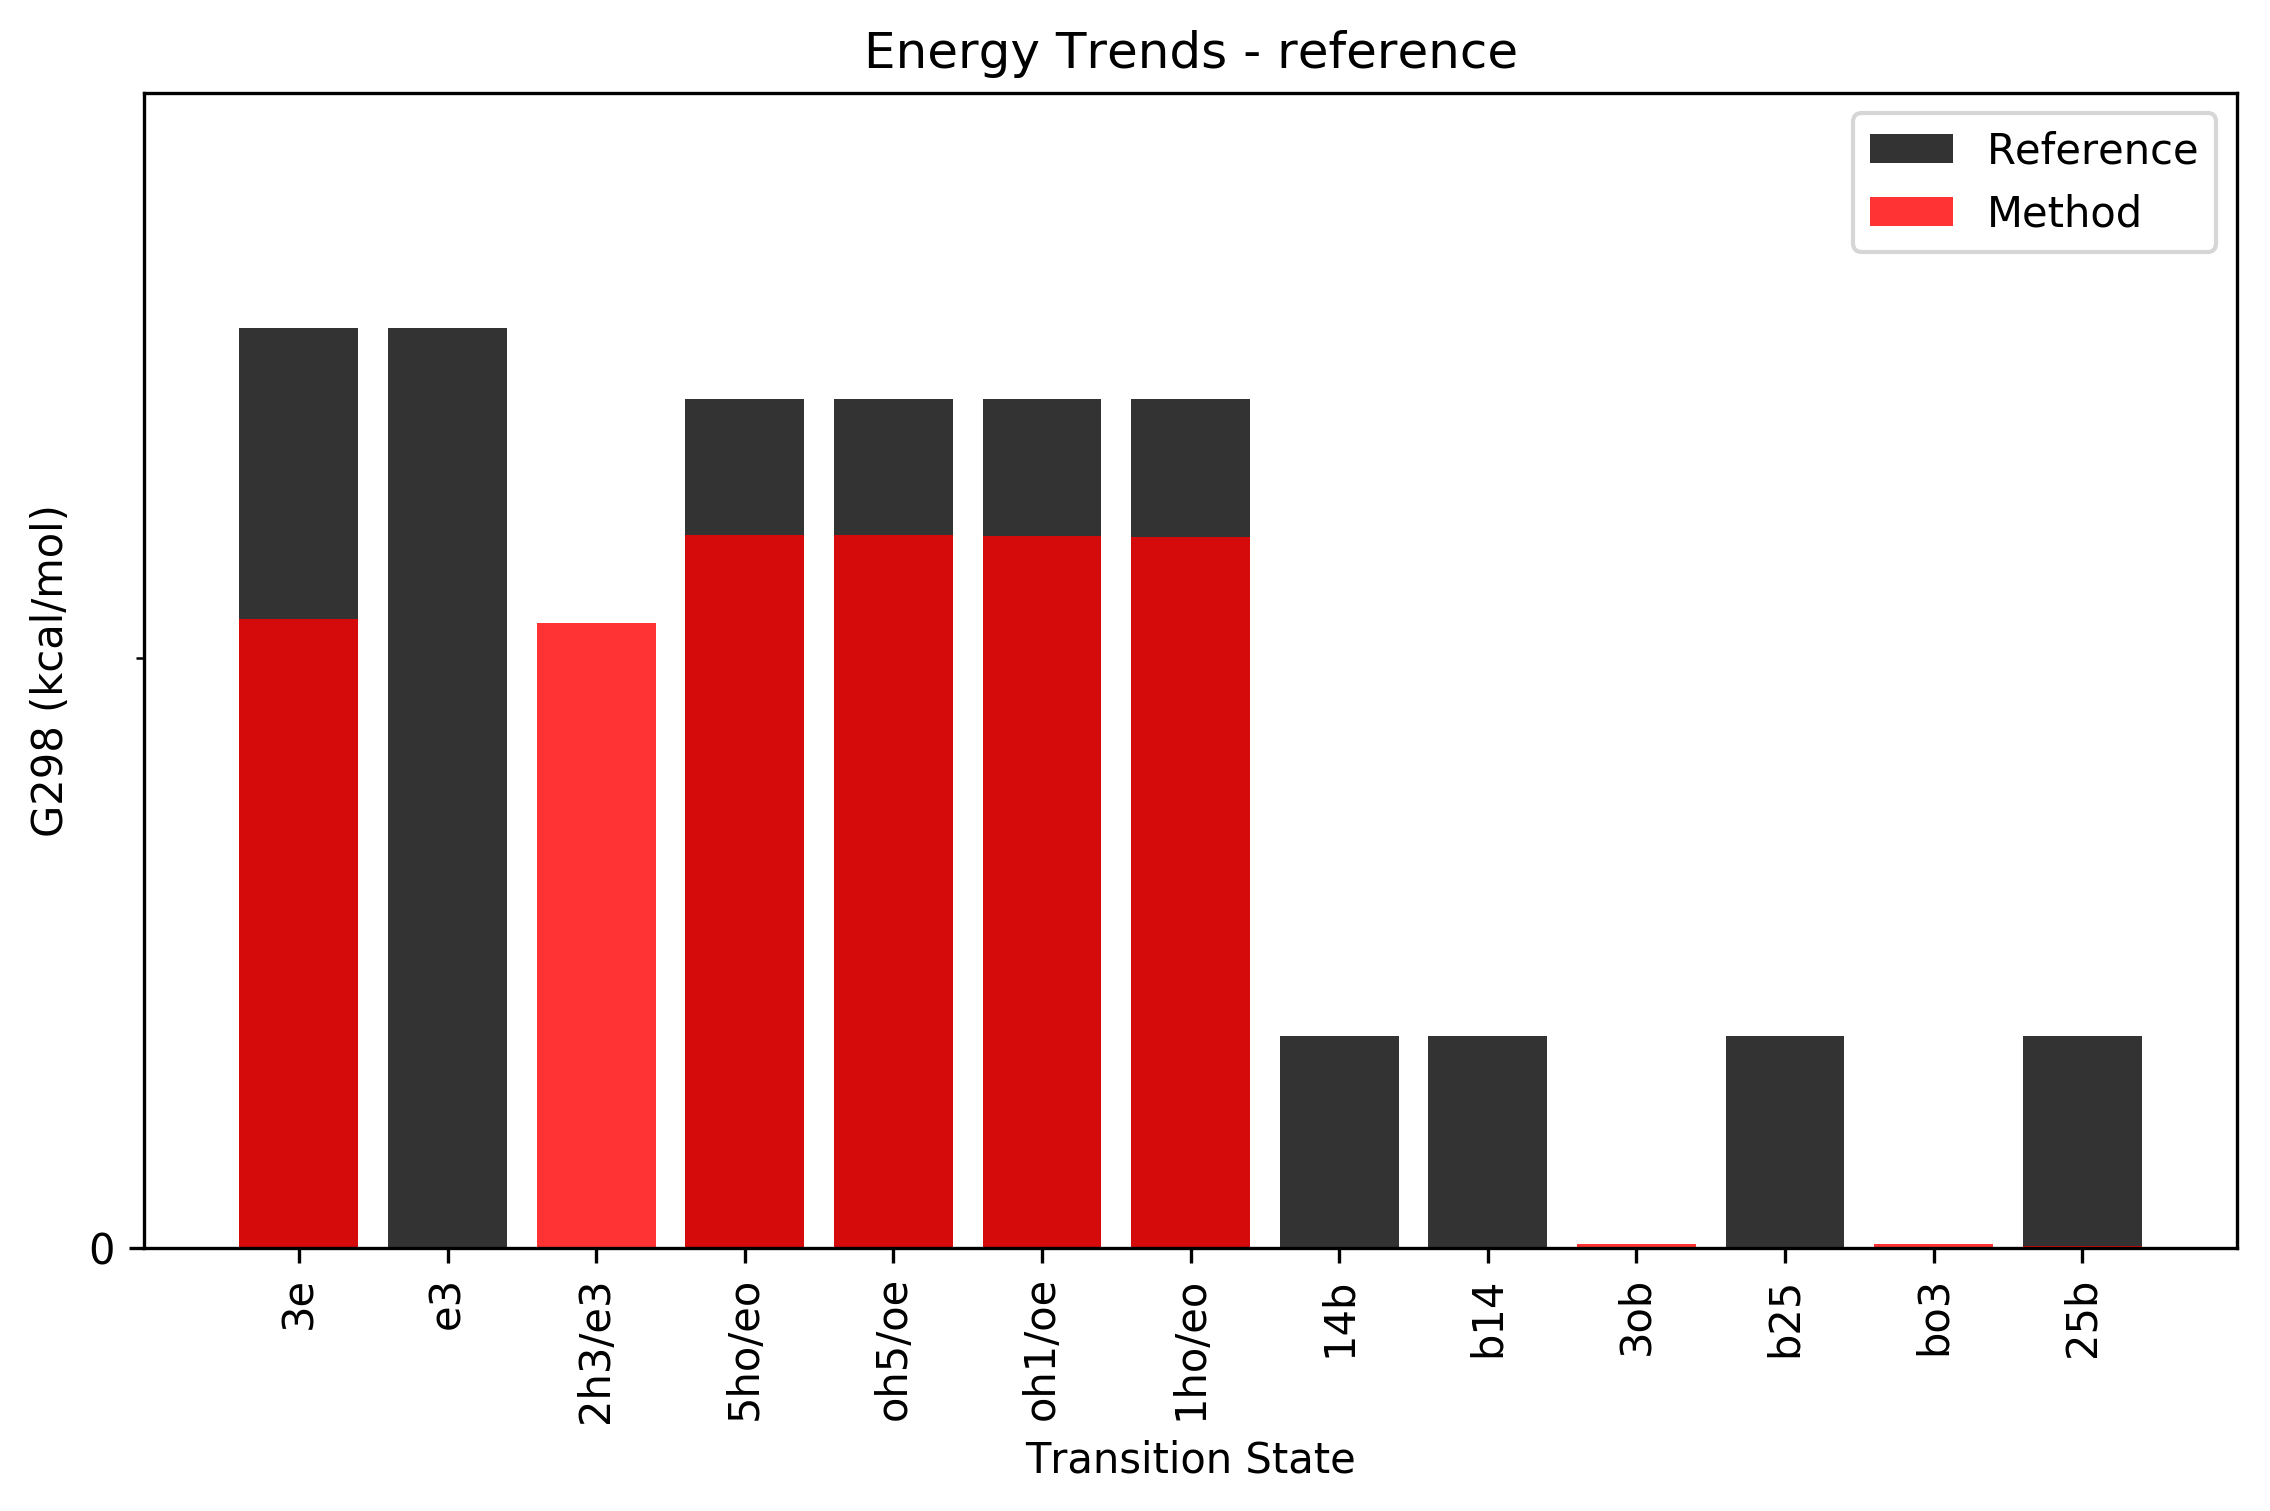
\includegraphics[width=1\textwidth,keepaspectratio]
		{figures/oxane/comp_tables/oxane-diff-trend-dftb.png}
		\caption{DFTB}
	\end{subfigure}
	~
	\begin{subfigure}[b]{0.3\textwidth}
		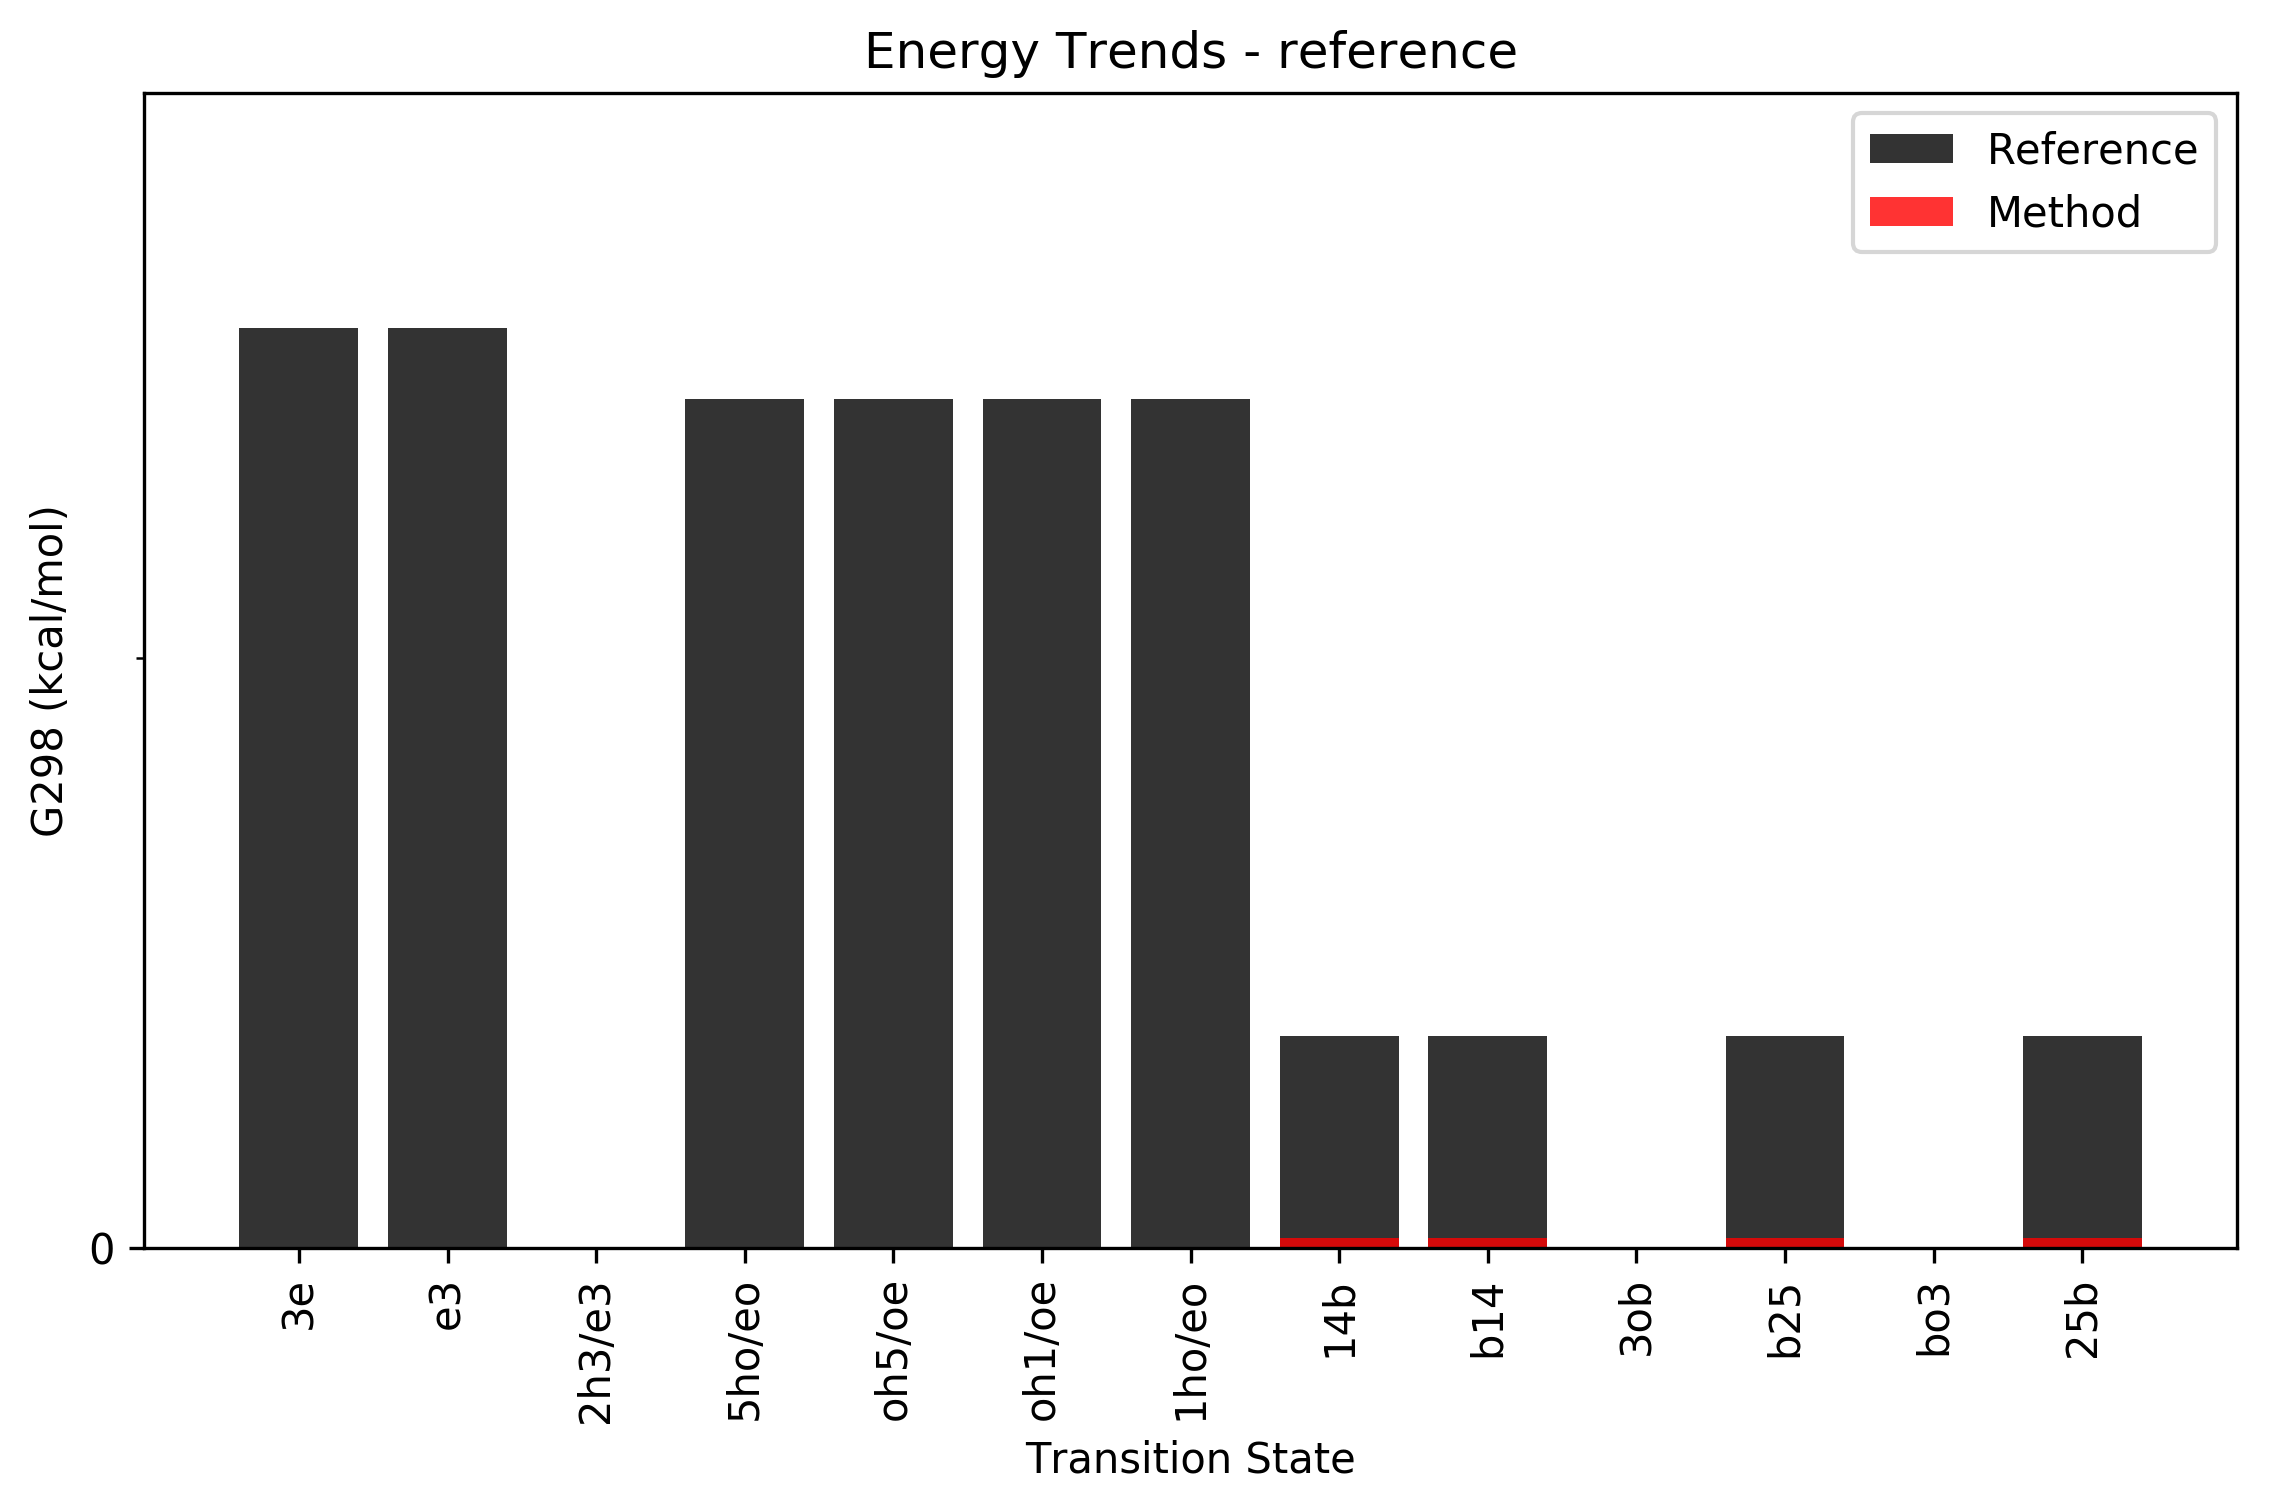
\includegraphics[width=1\textwidth,keepaspectratio]
		{figures/oxane/comp_tables/oxane-diff-trend-am1.png}
		\caption{AM1}
	\end{subfigure}
	
	\begin{subfigure}[b]{0.3\textwidth}
		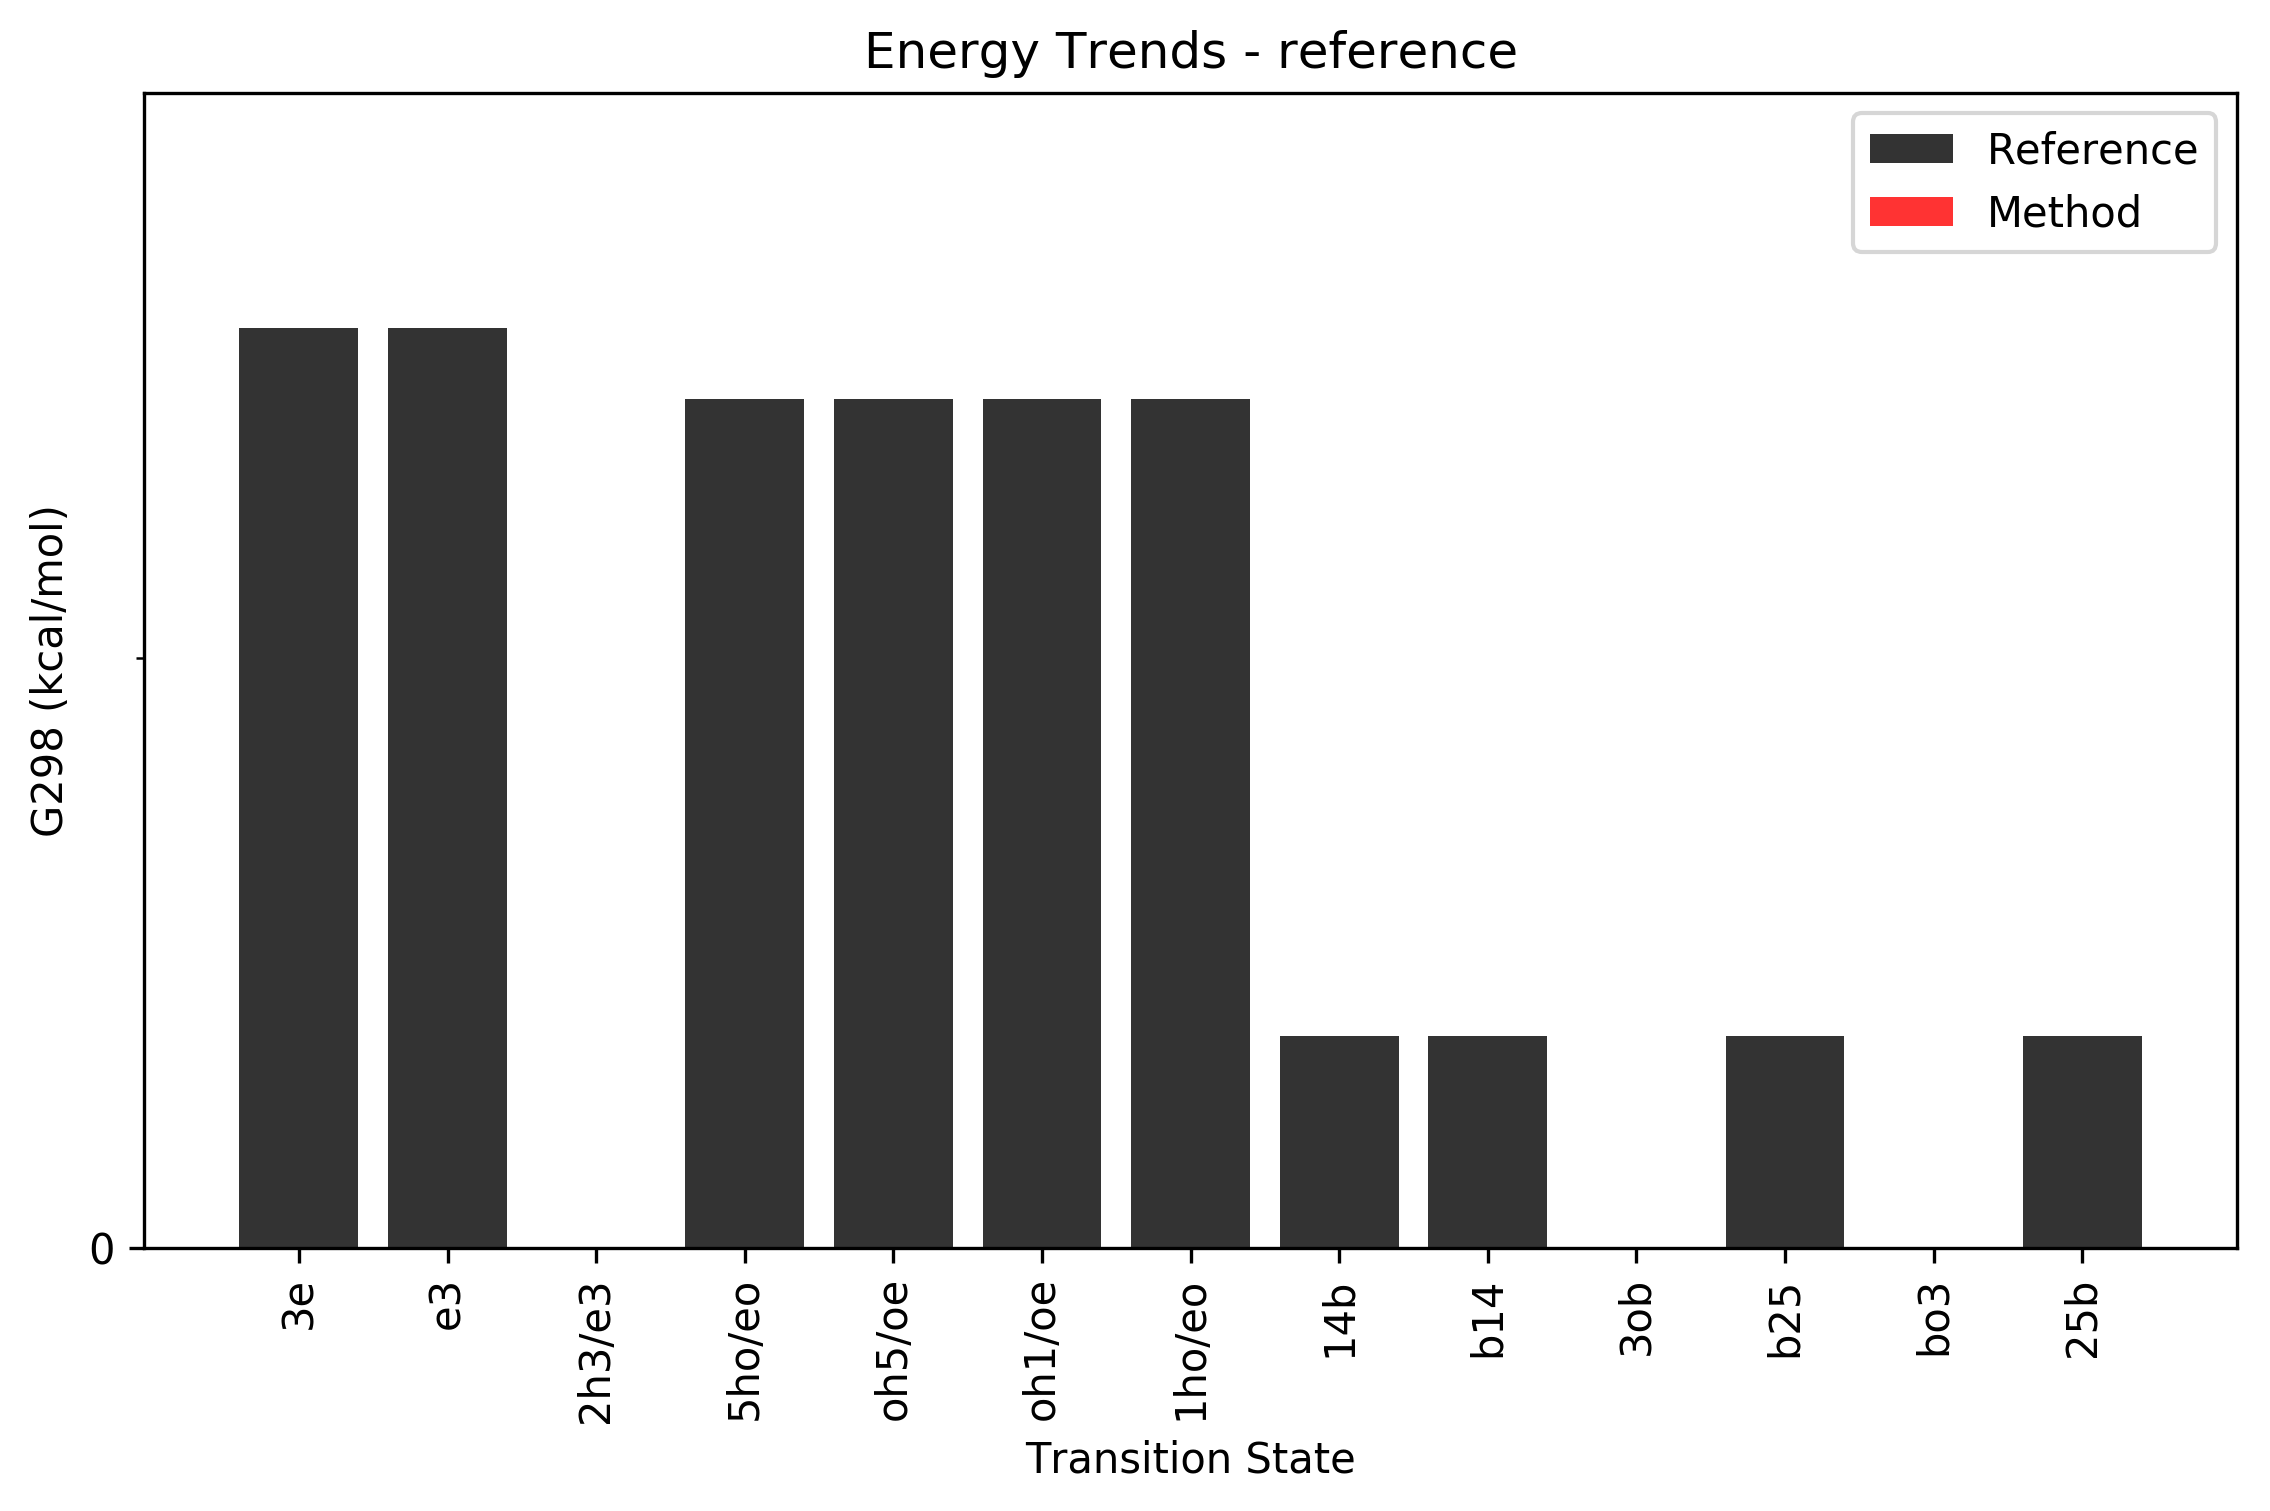
\includegraphics[width=1\textwidth,keepaspectratio]
		{figures/oxane/comp_tables/oxane-diff-trend-pm3.png}
		\caption{PM3}
	\end{subfigure}
	~
	\begin{subfigure}[b]{0.3\textwidth}
		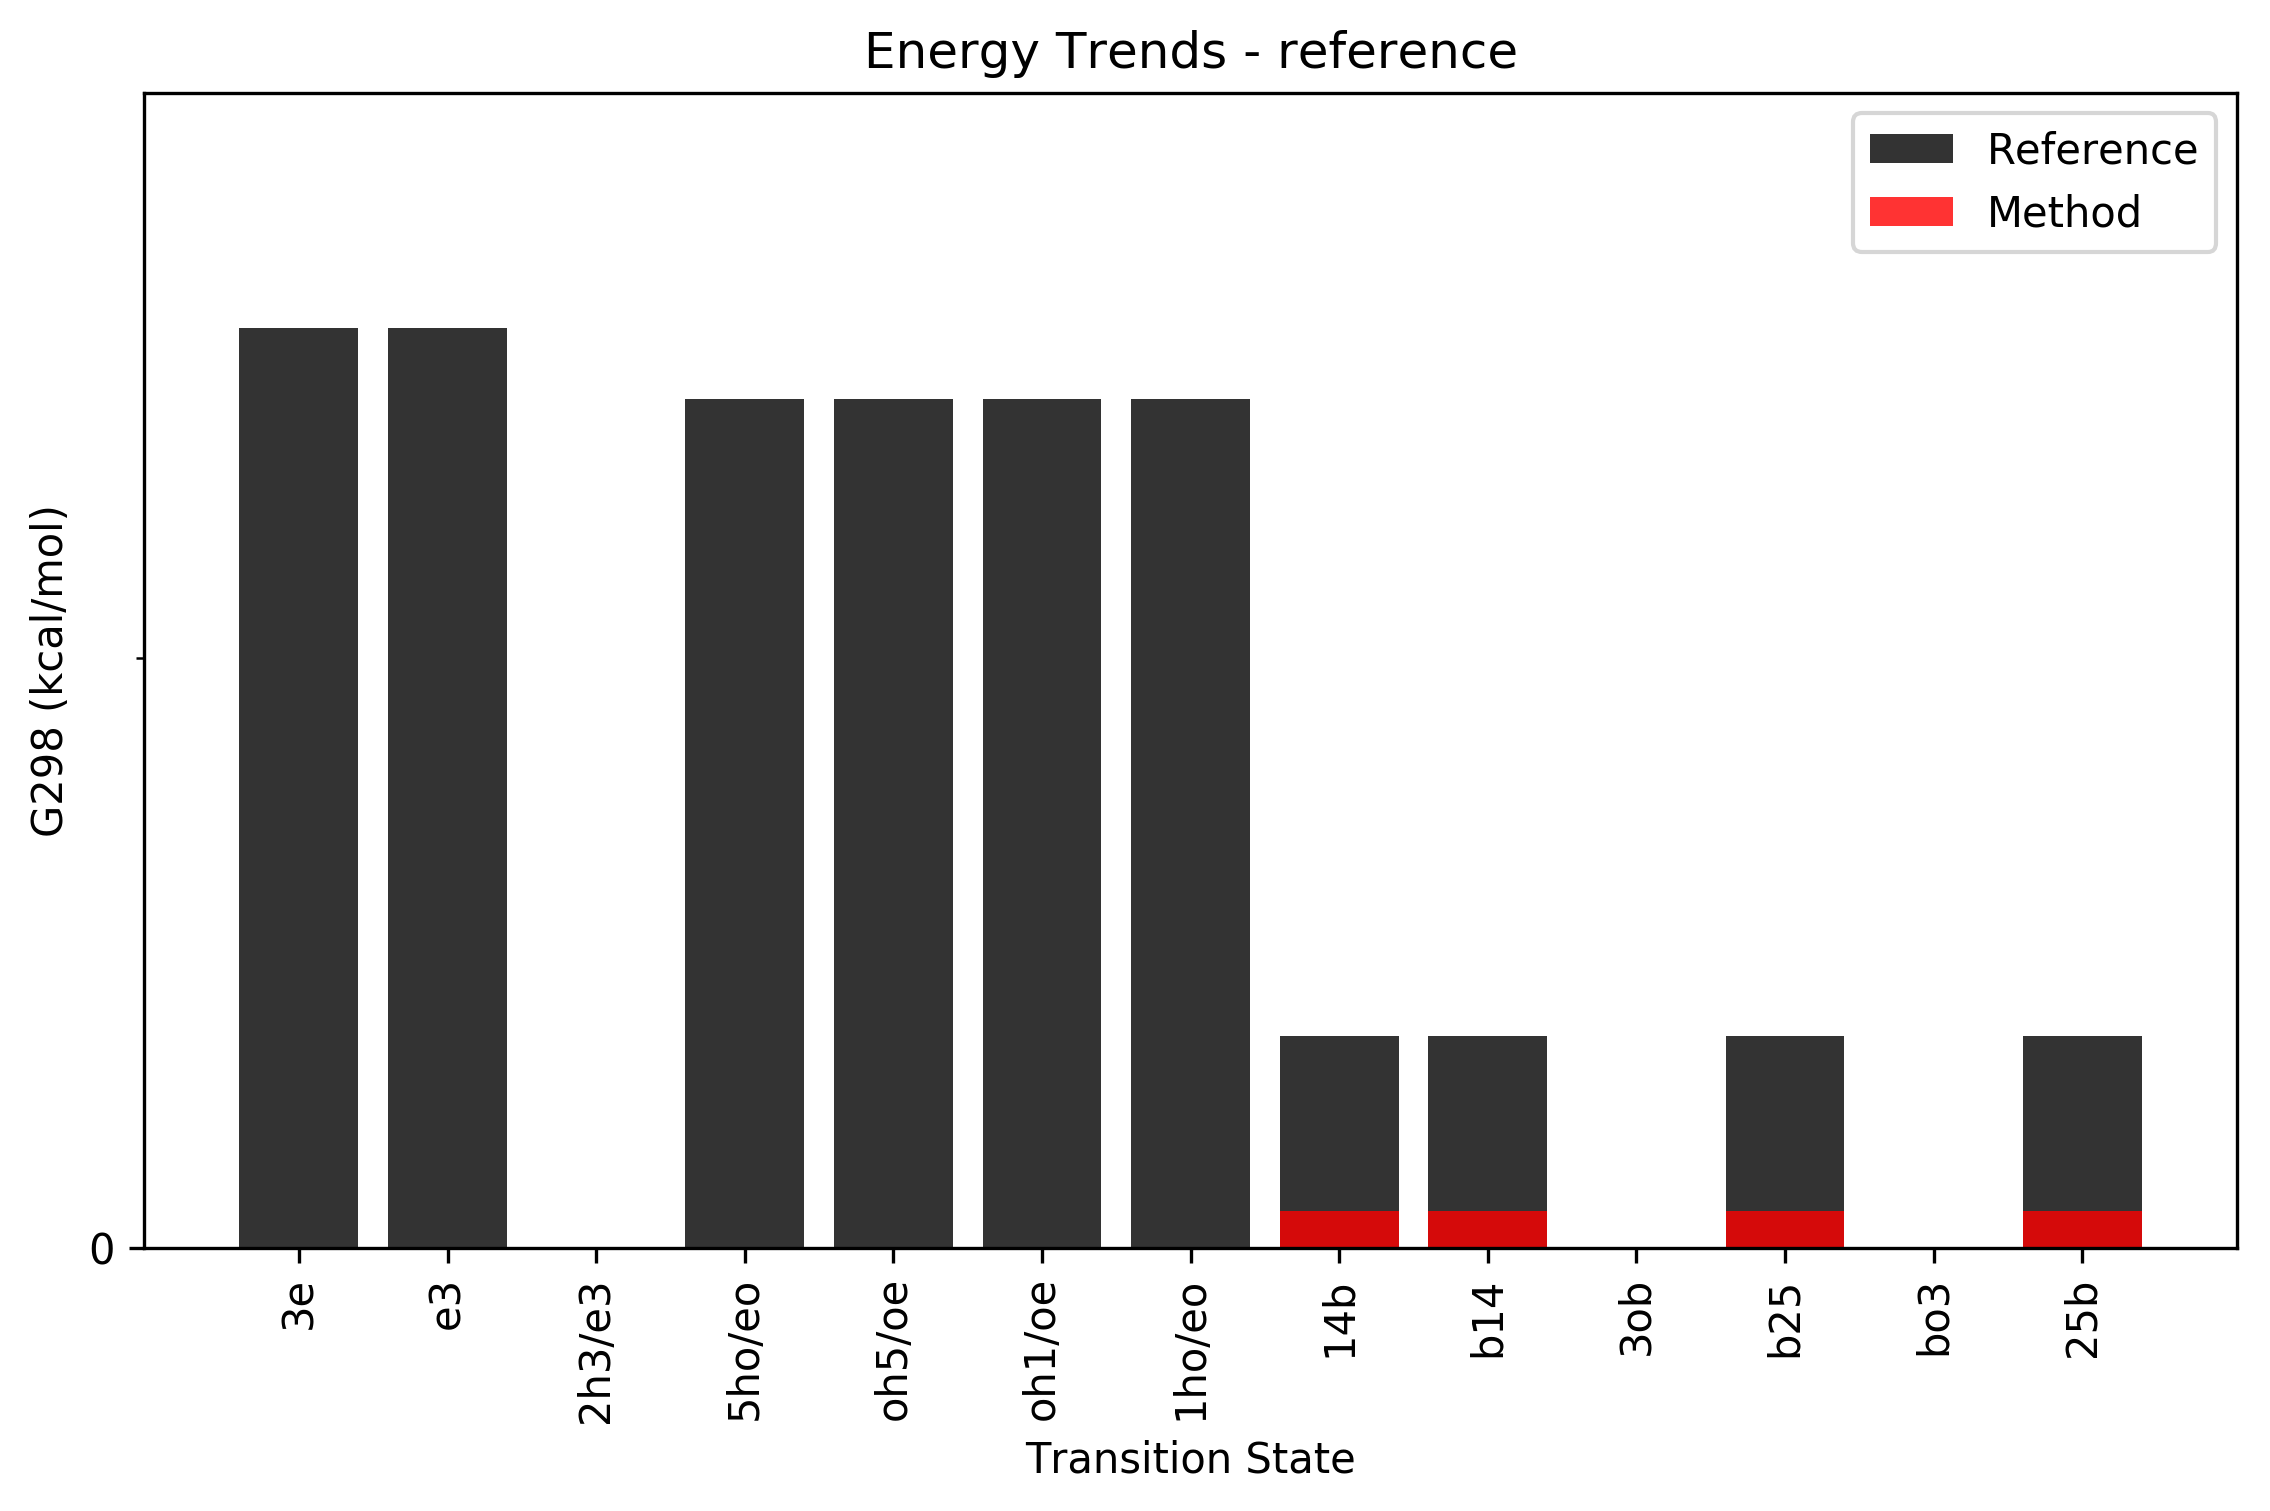
\includegraphics[width=1\textwidth,keepaspectratio]
		{figures/oxane/comp_tables/oxane-diff-trend-pm3mm.png}
		\caption{PM3MM}
	\end{subfigure}
	~
	\begin{subfigure}[b]{0.3\textwidth}
		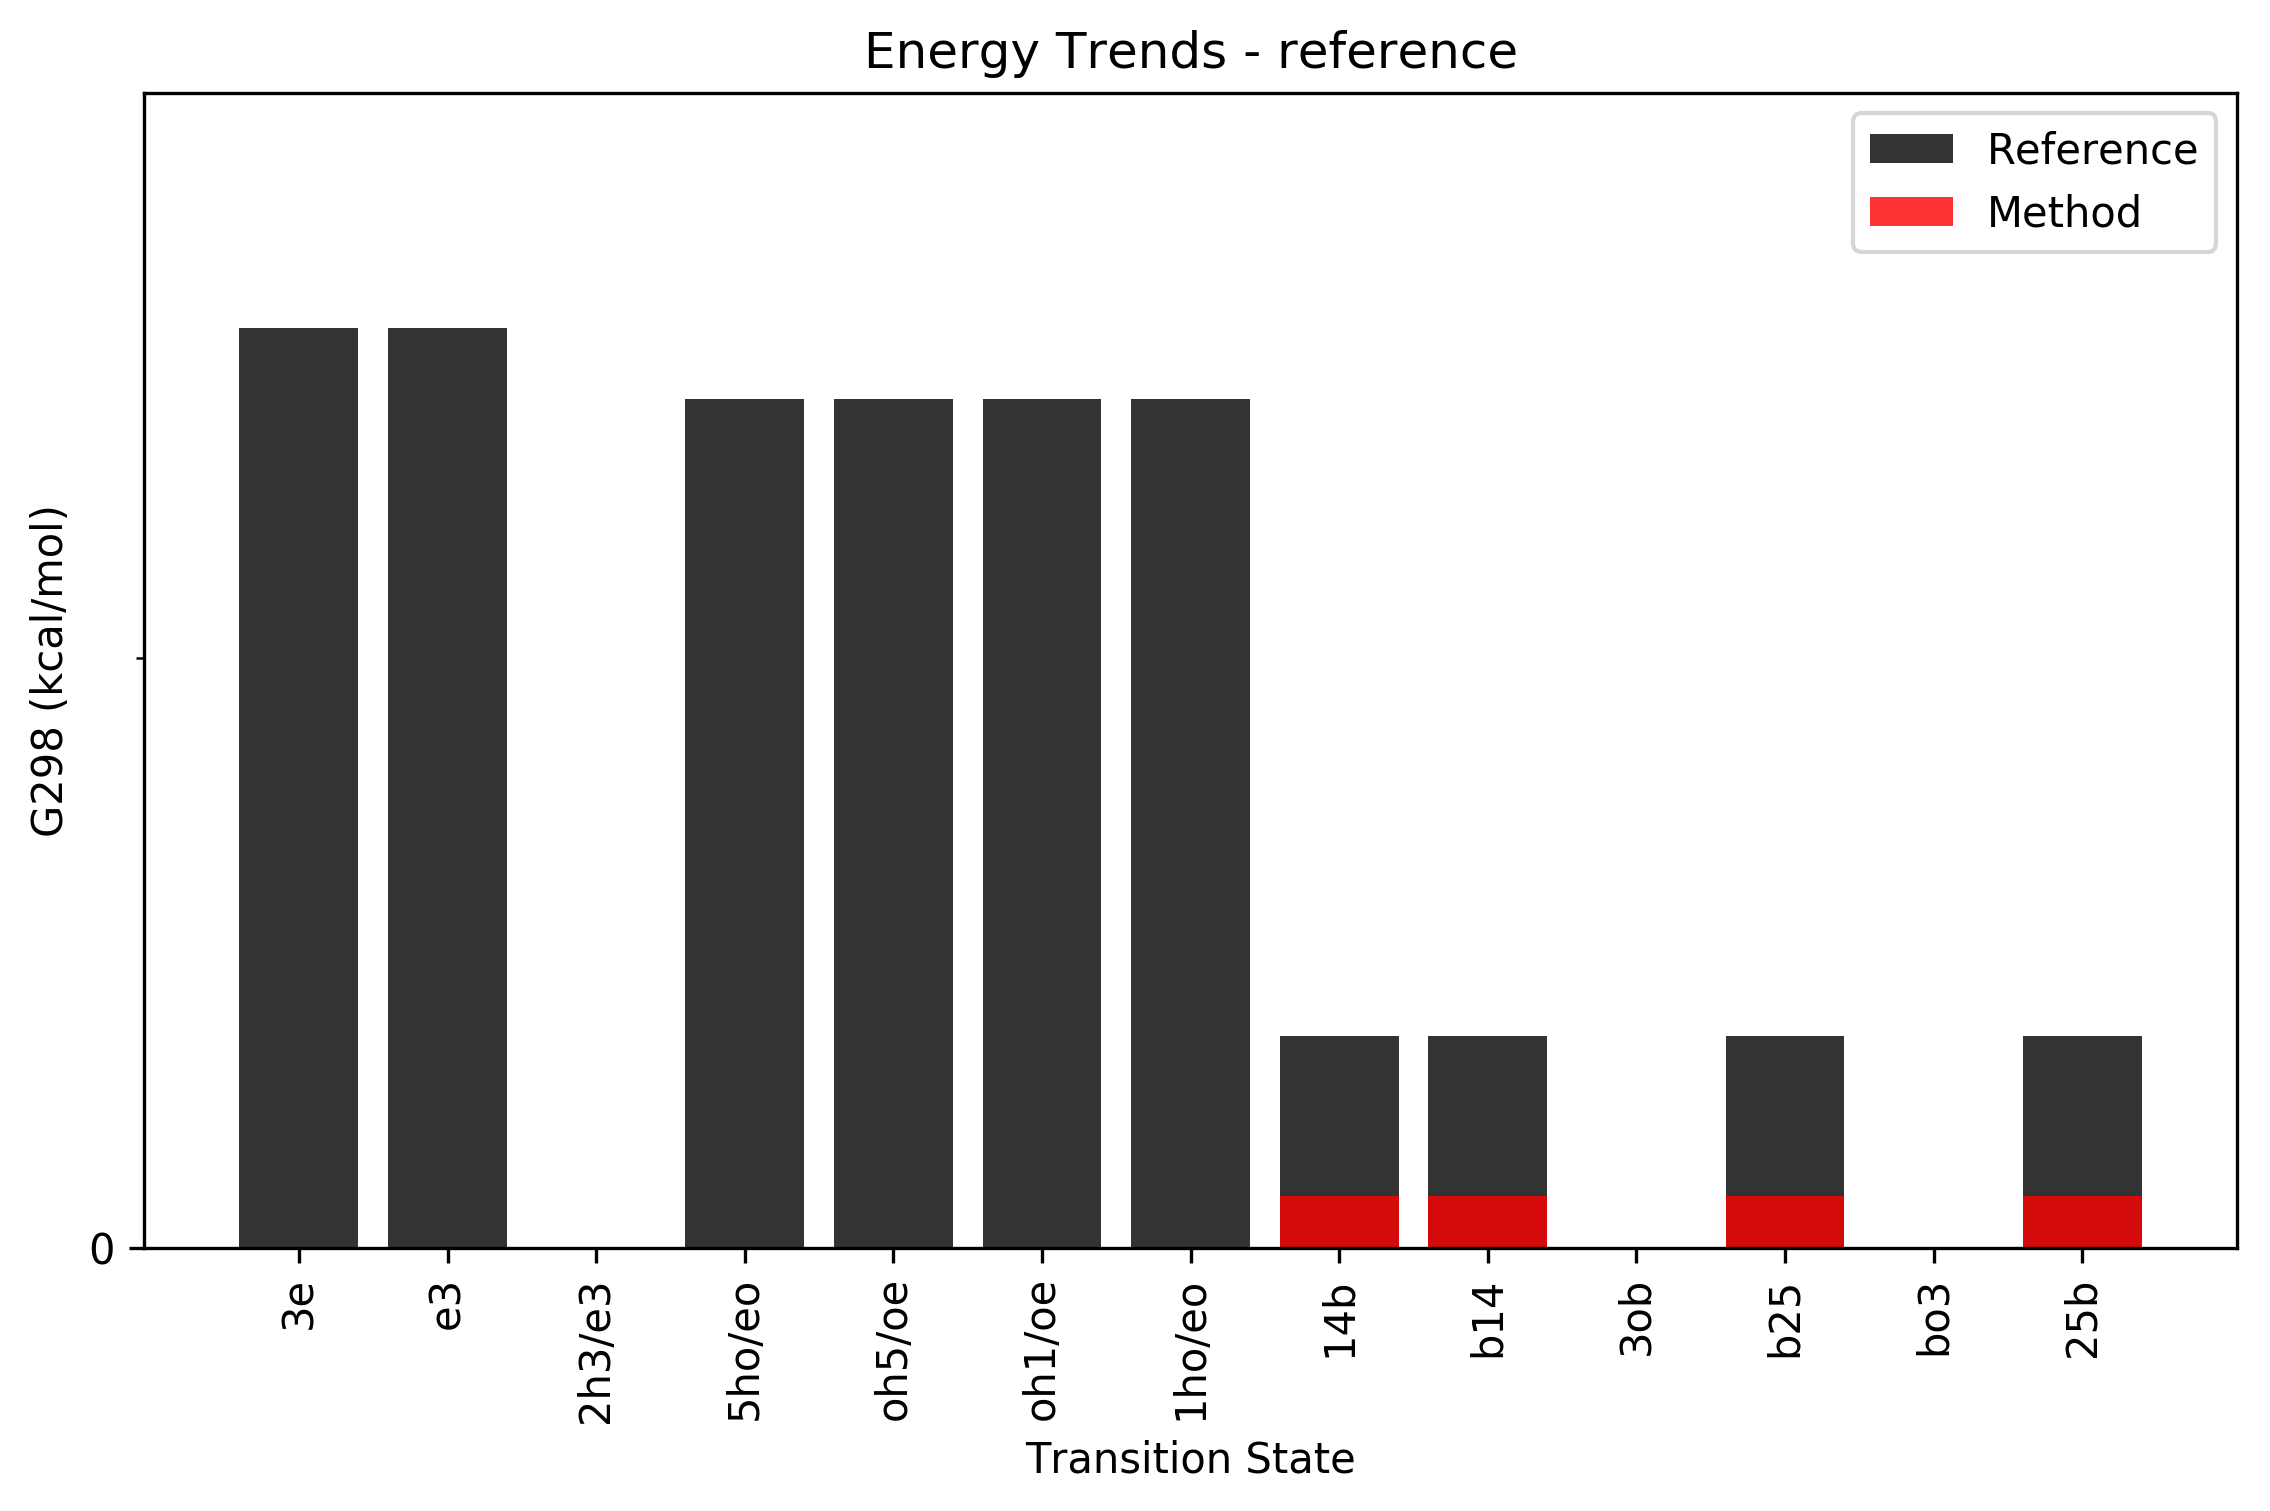
\includegraphics[width=1\textwidth,keepaspectratio]
		{figures/oxane/comp_tables/oxane-diff-trend-pm6.png}
		\caption{PM6}
	\end{subfigure}
\caption{\hl{Insert Caption}}
\label{fig:oxane-ALL-LM}
\end{figure}



\newpage
% % % % % % % % % % % 
% % % Beta-xylose  % % % 
% % % % % % % % % % %
\subsection{\textbeta-Xylose}
The next conformational landscape explored was \textbeta-xylose, which contains four hydroxyl groups. The addition of 
these hydroxyl groups allows for the ring to adopt a variety of conformations. 

\subsubsection{Local Minima Reference Landscape}
To compare the conformational landscapes across different methods for \textbeta-xylose, we initially generated a set of reference landscapes 
based on the work of Mayes et al. (as discussed in the Computational Methods: Generating Reference Landscapes section). Figure 
\ref{fig:bxyl-ref-LM} shows the LM k-mean centers (red) for the reference structures as well as the voronoi edges (green) and the raw data 
from Mayes et al. (blue). For \textbeta-xylose, nine LM k-means centers were used to capture the conformational landscape of Mayes et al. 
The max WRMSD for the reference landscape (5s1/25b) has a value of 0.092.

\begin{figure}[h!]
  	\centering
  	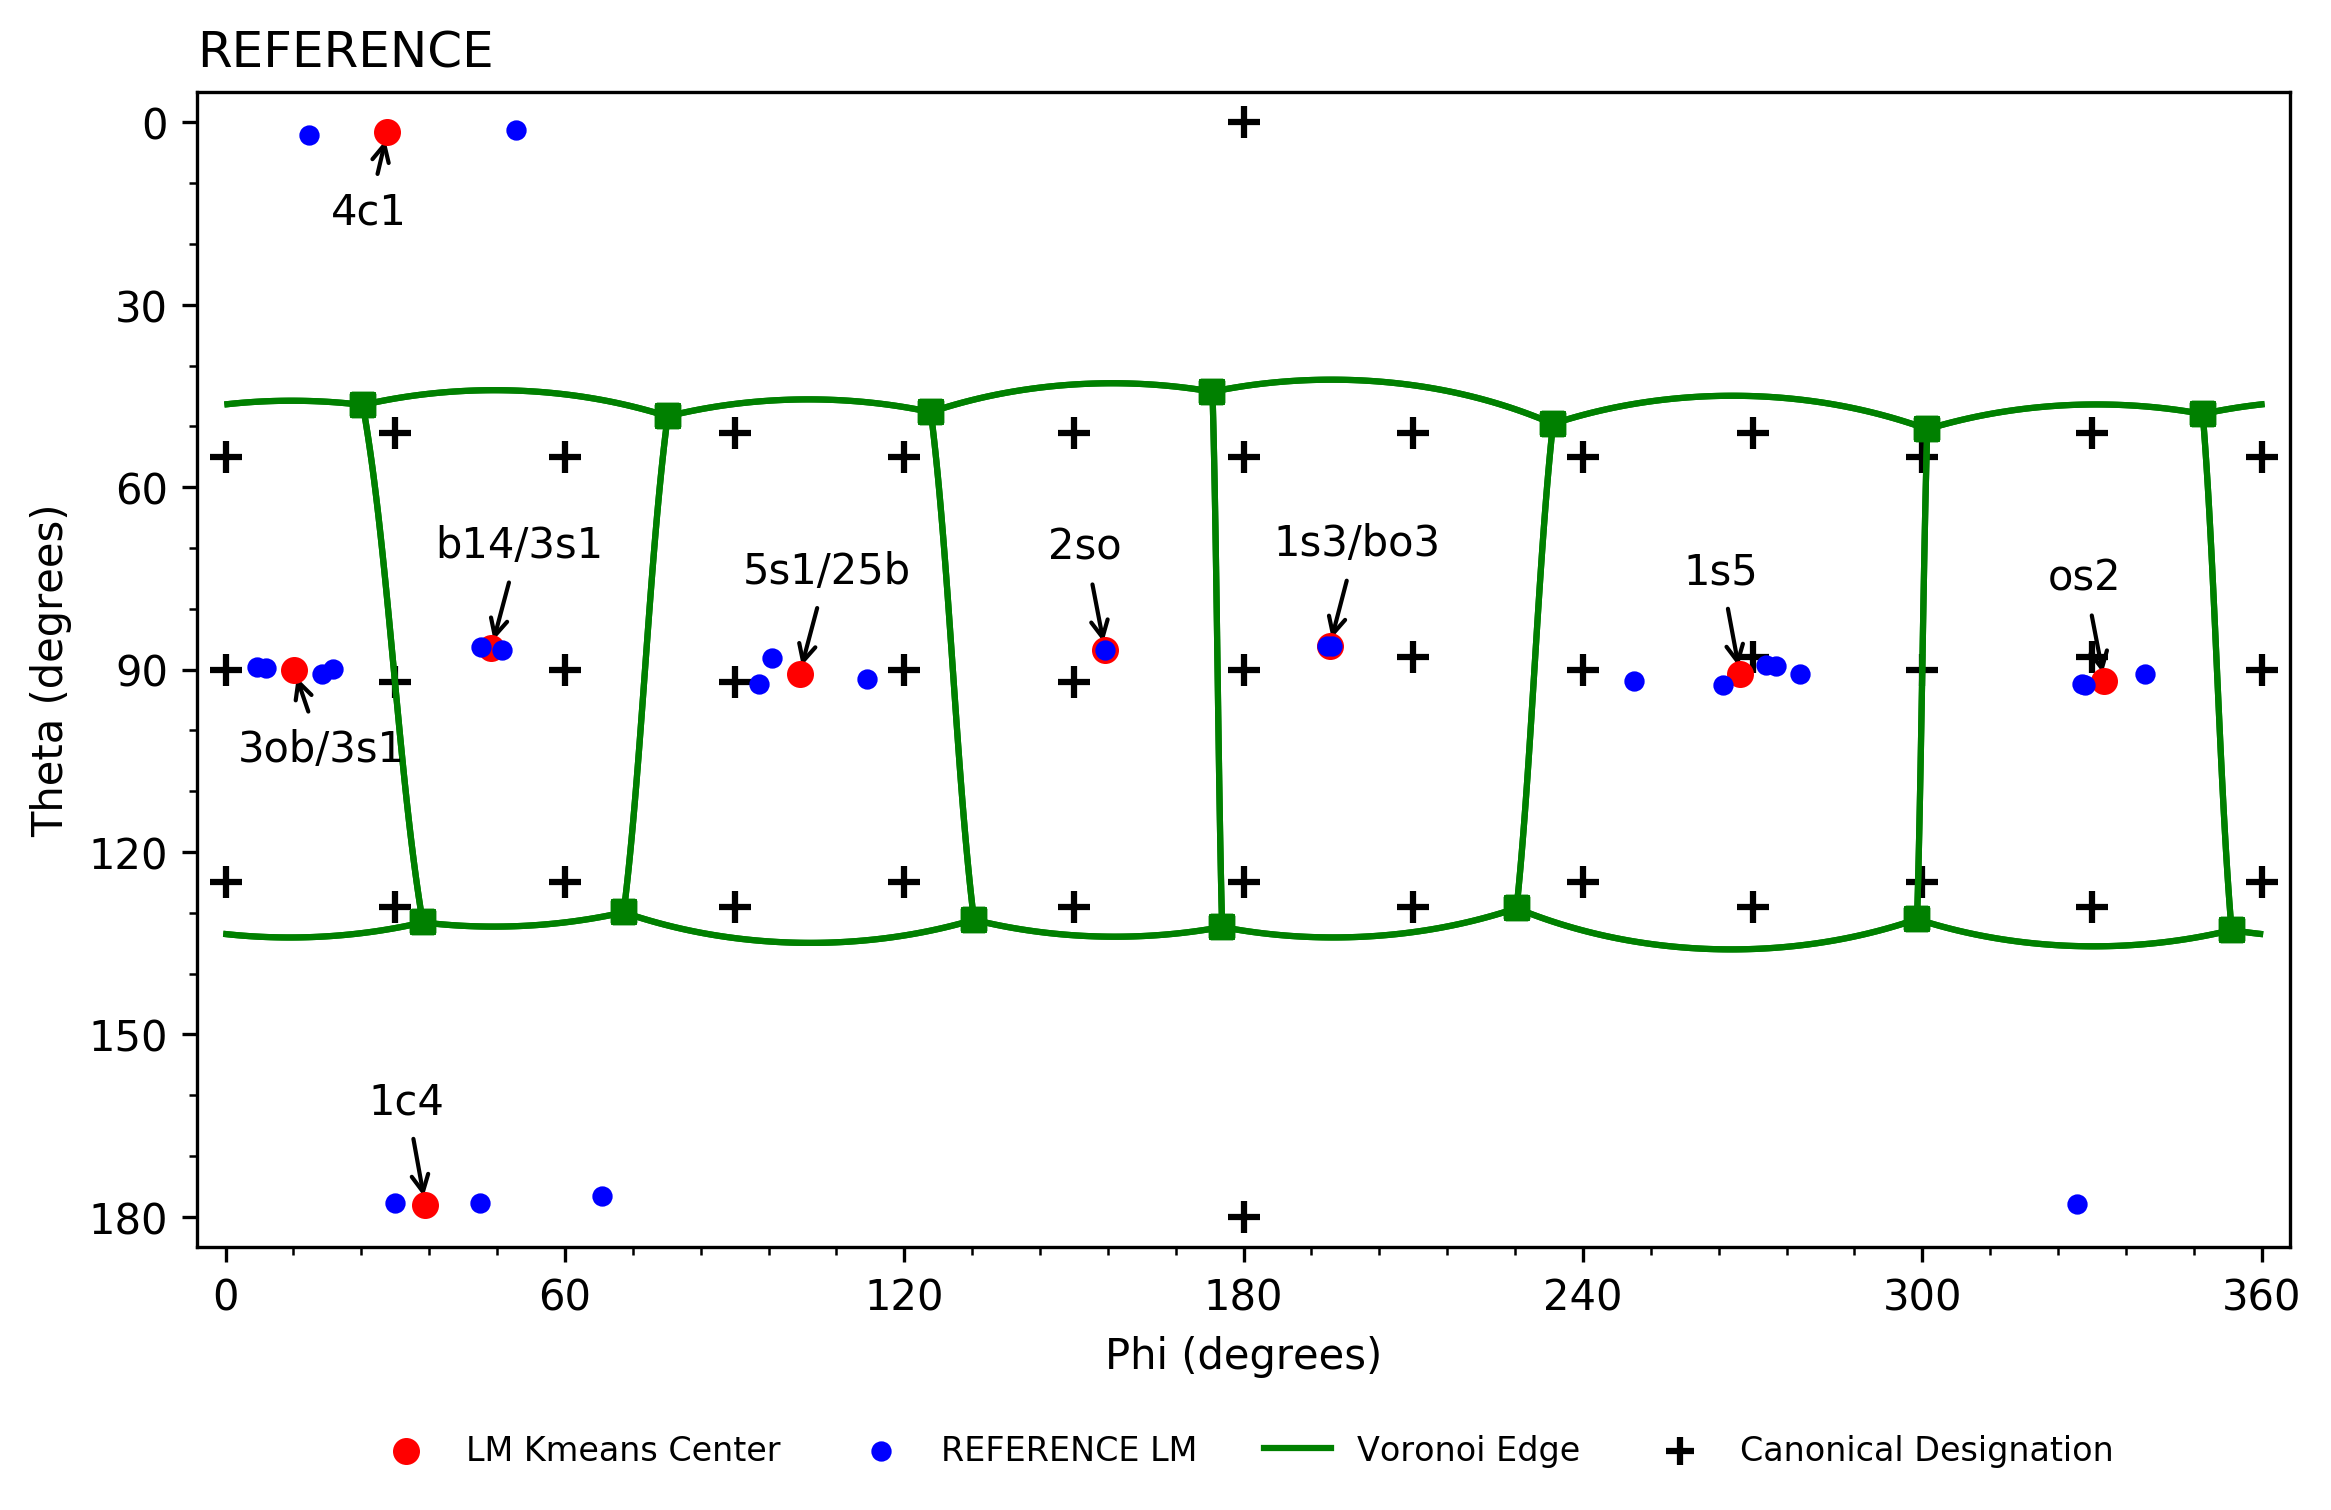
\includegraphics[width=\textwidth,height=\textheight,keepaspectratio]
	{figures/bxyl/overall/z_dataset-bxyl-LM-REFERENCE-all_groupings.png}
	\caption{The LM reference landscape for \textbeta-xylose.}
 	\label{fig:bxyl-ref-LM}
\end{figure}

\subsubsection{Transition State Reference Landscape}
With the LM conformational landscape for \textbeta-xylose generated, the TS connecting each LM were then determined. Each TS found in 
Figures \ref{fig:bxyl-ref-TS} and \ref{fig:bxyl-ref-TS-color} represent a unique structure connecting two LMs. To aid in visualization, Northern 
and Southern hemisphere plots were created to highlight the key pathways from 4c1 and 1c4 conformations. To distinguish the different 
pathways, each individual pathway was colored coded (Figure \ref{fig:bxyl-ref-TS-color}). 

Figure
\ref{fig:oxane-ref-TS} represents a unique structure that connects two LM. To aid in visualization, Northern and Southern hemisphere plots
were created to highlight key pathways from 4c1 and 1c4 conformations.

\begin{figure}[H]
  	\centering
  	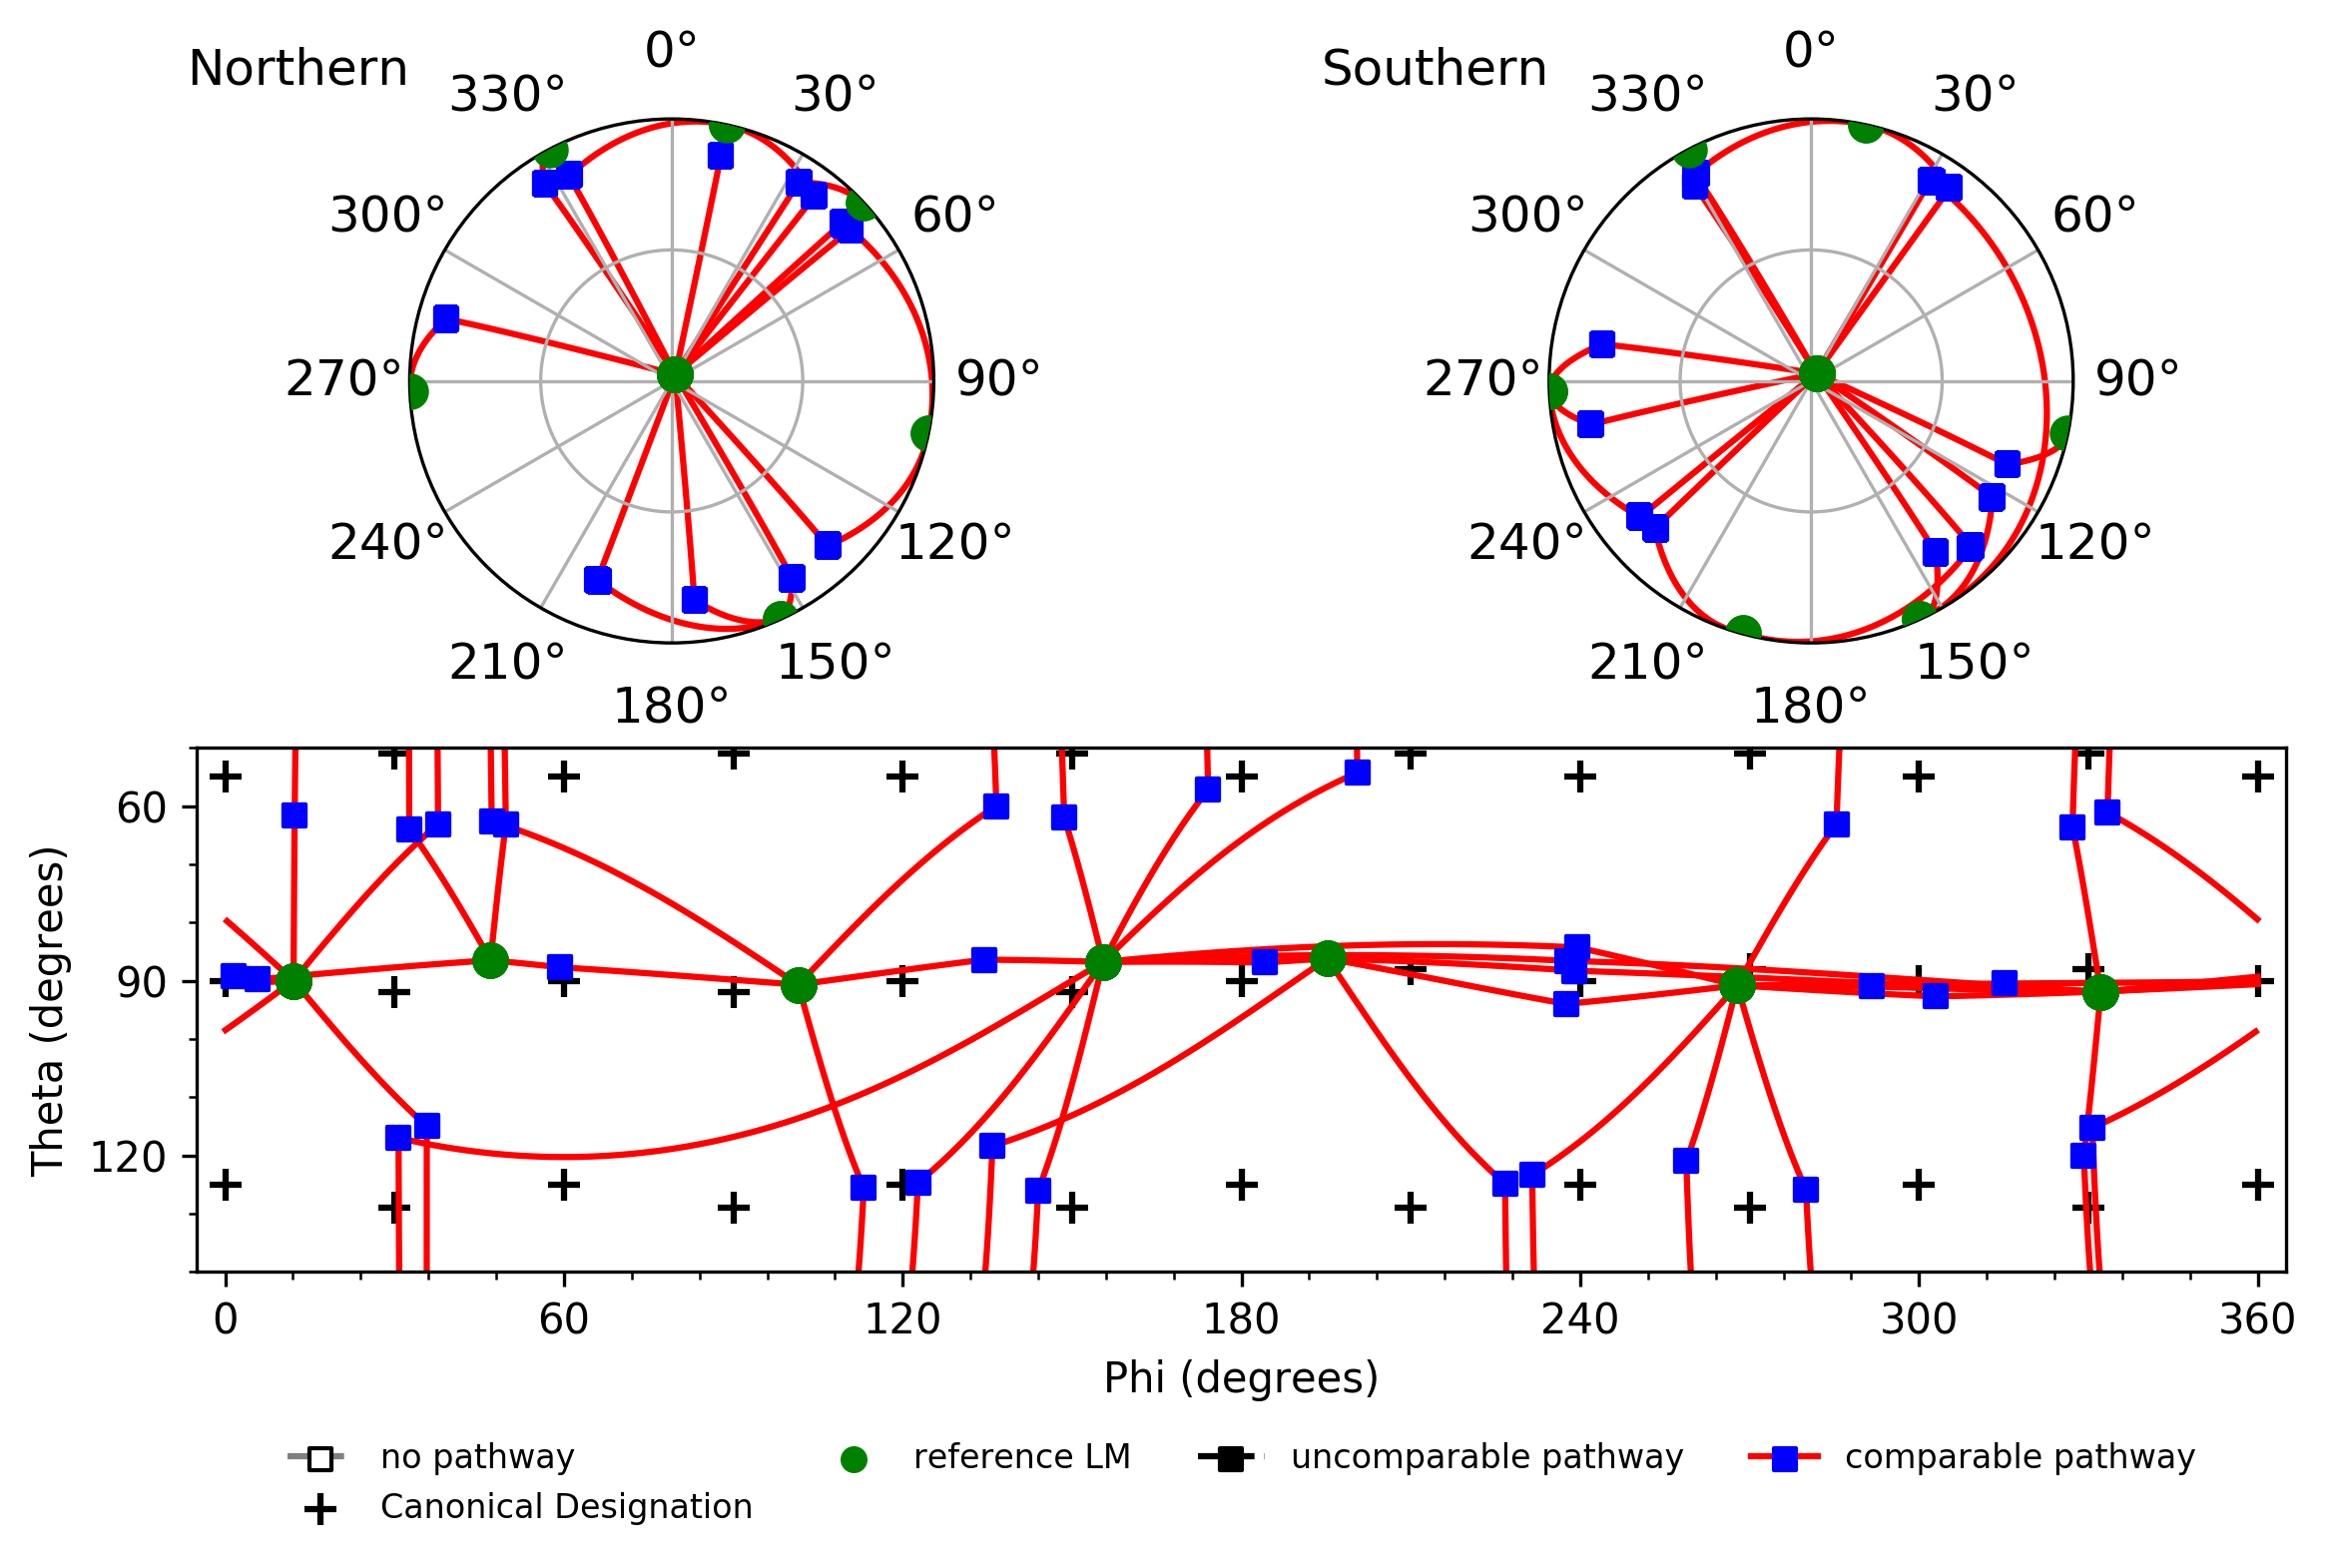
\includegraphics[width=\textwidth,height=\textheight,keepaspectratio]
	{figures/bxyl/z_dataset-bxyl-TS-WRMSD-comp-reference.png}
	\caption{The TS reference landscape for \textbeta-xylose.}
 	\label{fig:bxyl-ref-TS}
\end{figure}

\begin{figure}[H]
  	\centering
  	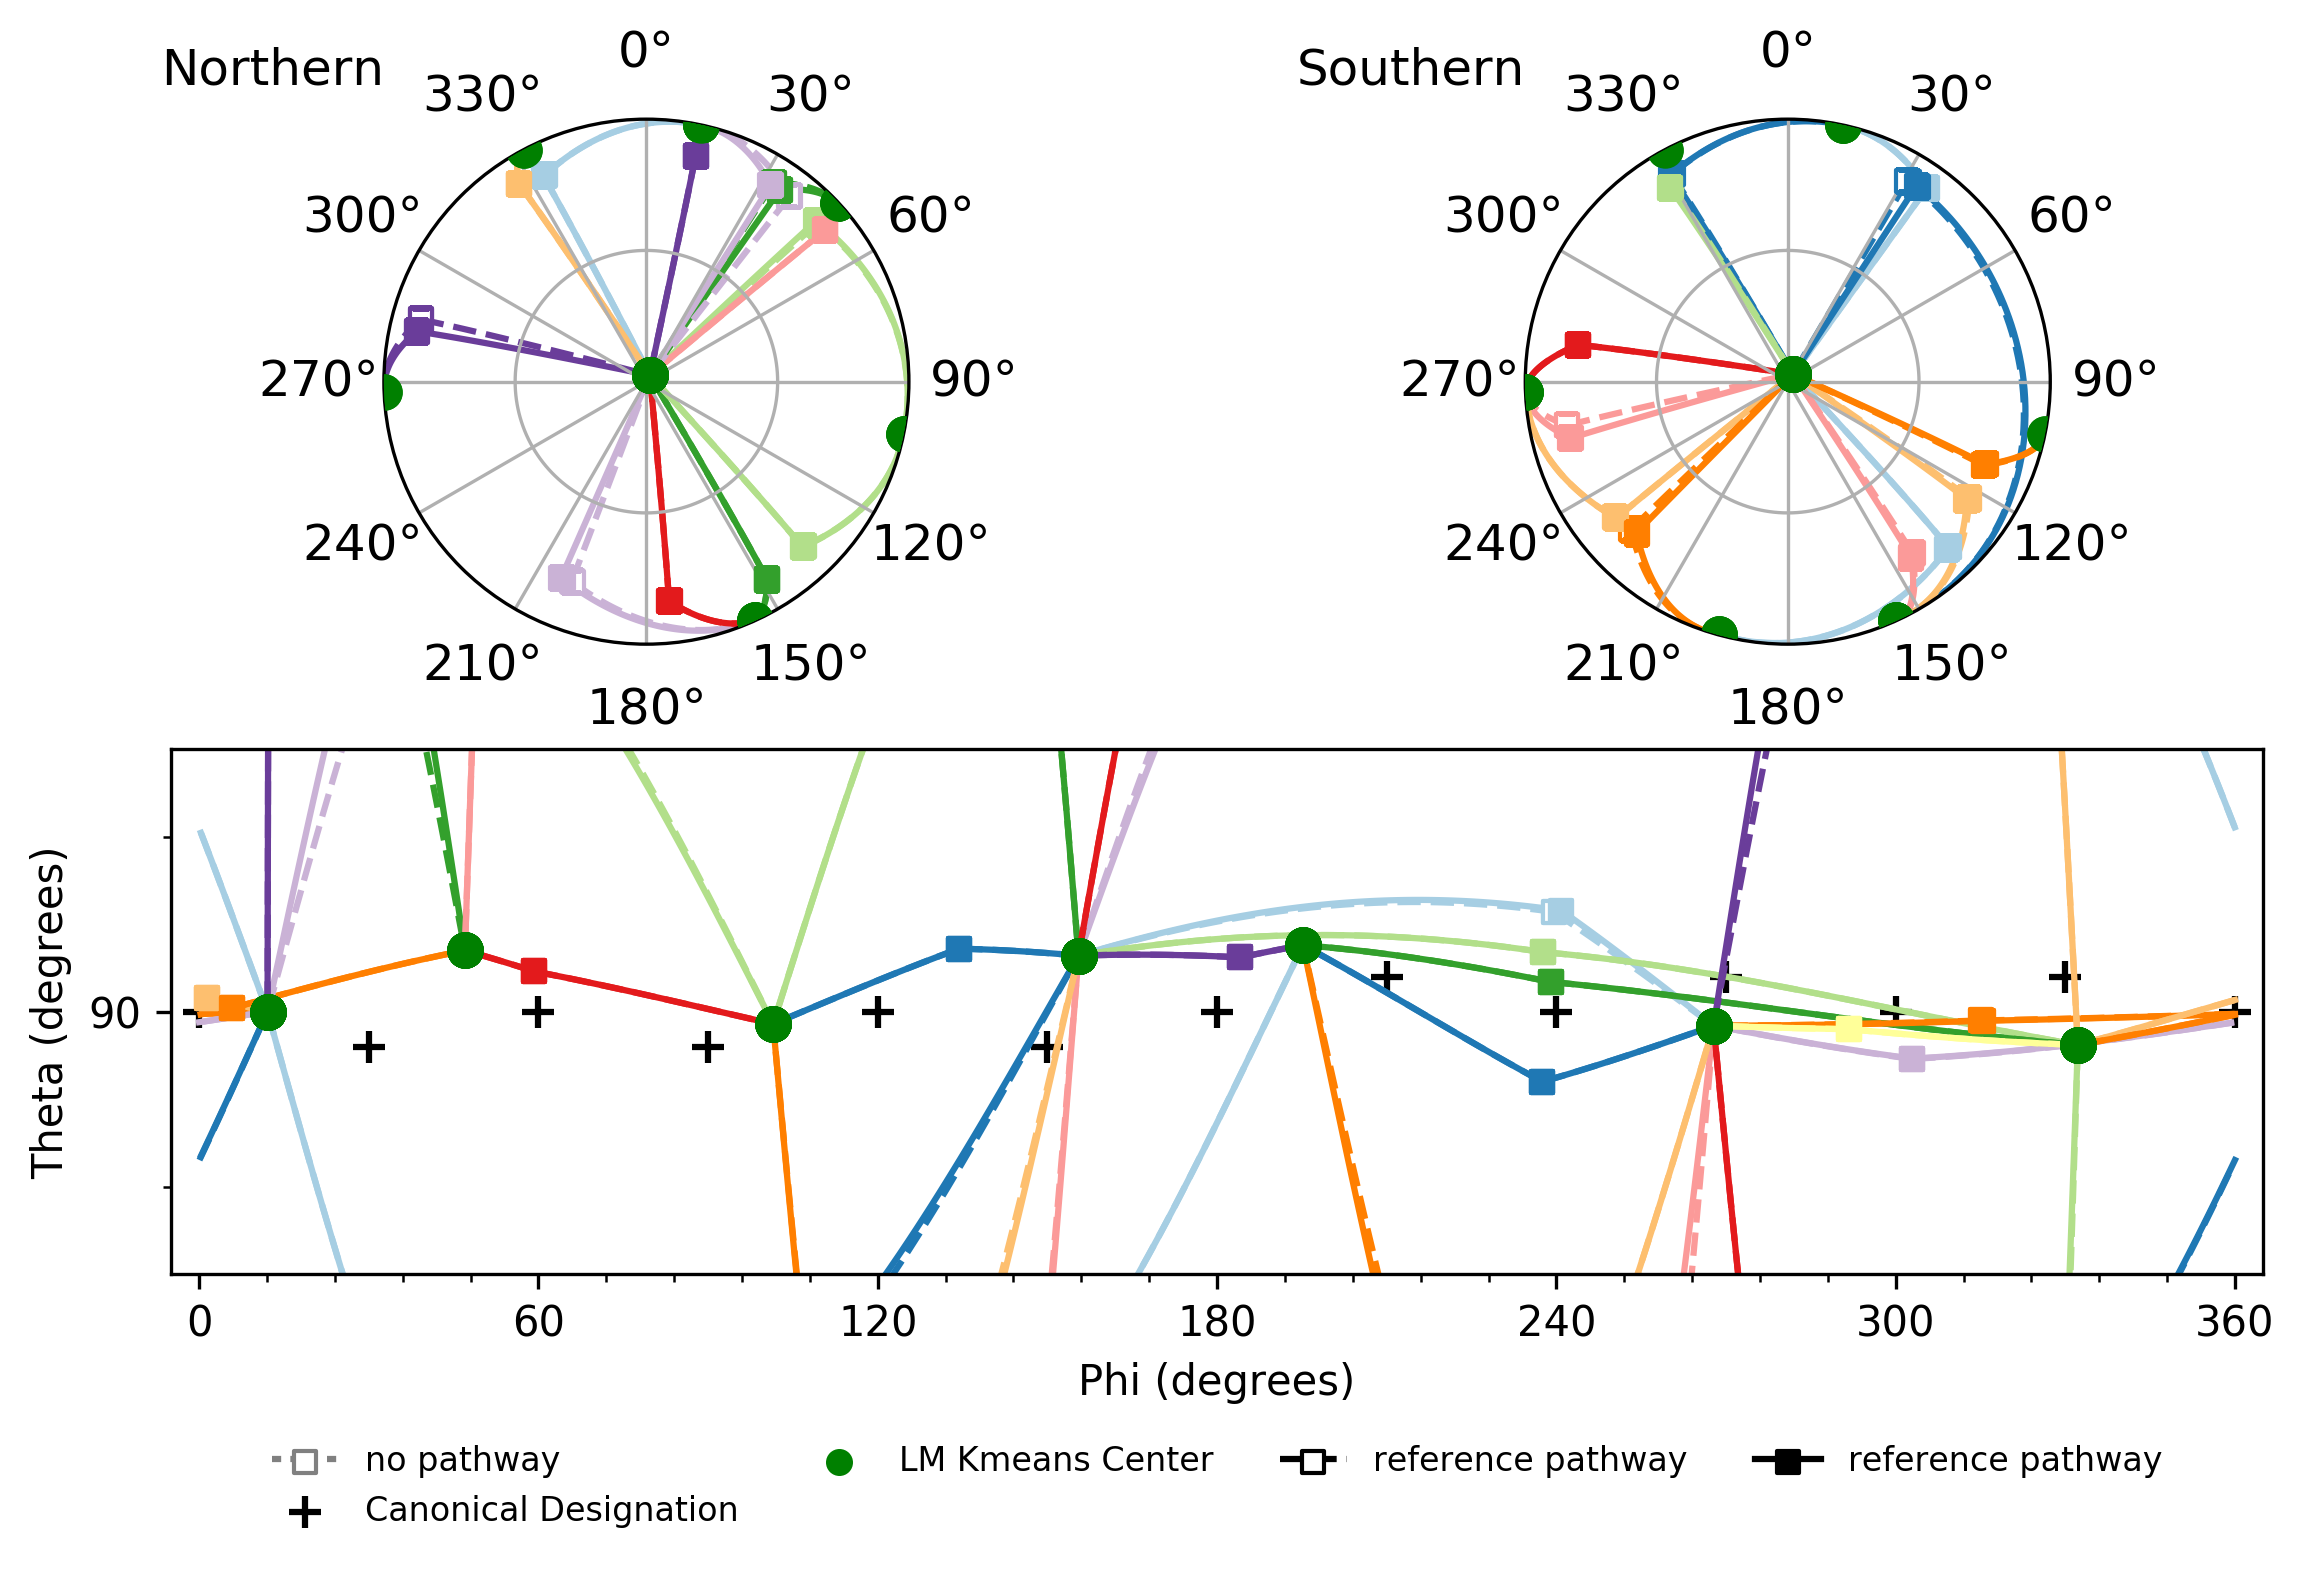
\includegraphics[width=\textwidth,height=\textheight,keepaspectratio]
	{figures/bxyl/z_dataset-bxyl-TS--all_groups_comp-reference.png}
	\caption{The TS reference landscape for \textbeta-xylose. Each pathway is colored individually to 
	show the interconnectivity. Also, note the difference in theta values for the equatorial image compared to Figure \ref{fig:bxyl-ref-TS}}.
 	\label{fig:bxyl-ref-TS-color}
\end{figure}



\subsubsection{Local Minima Landscapes}

\begin{figure}[H]
	\centering
   	\begin{subfigure}[b]{0.49\textwidth}
   	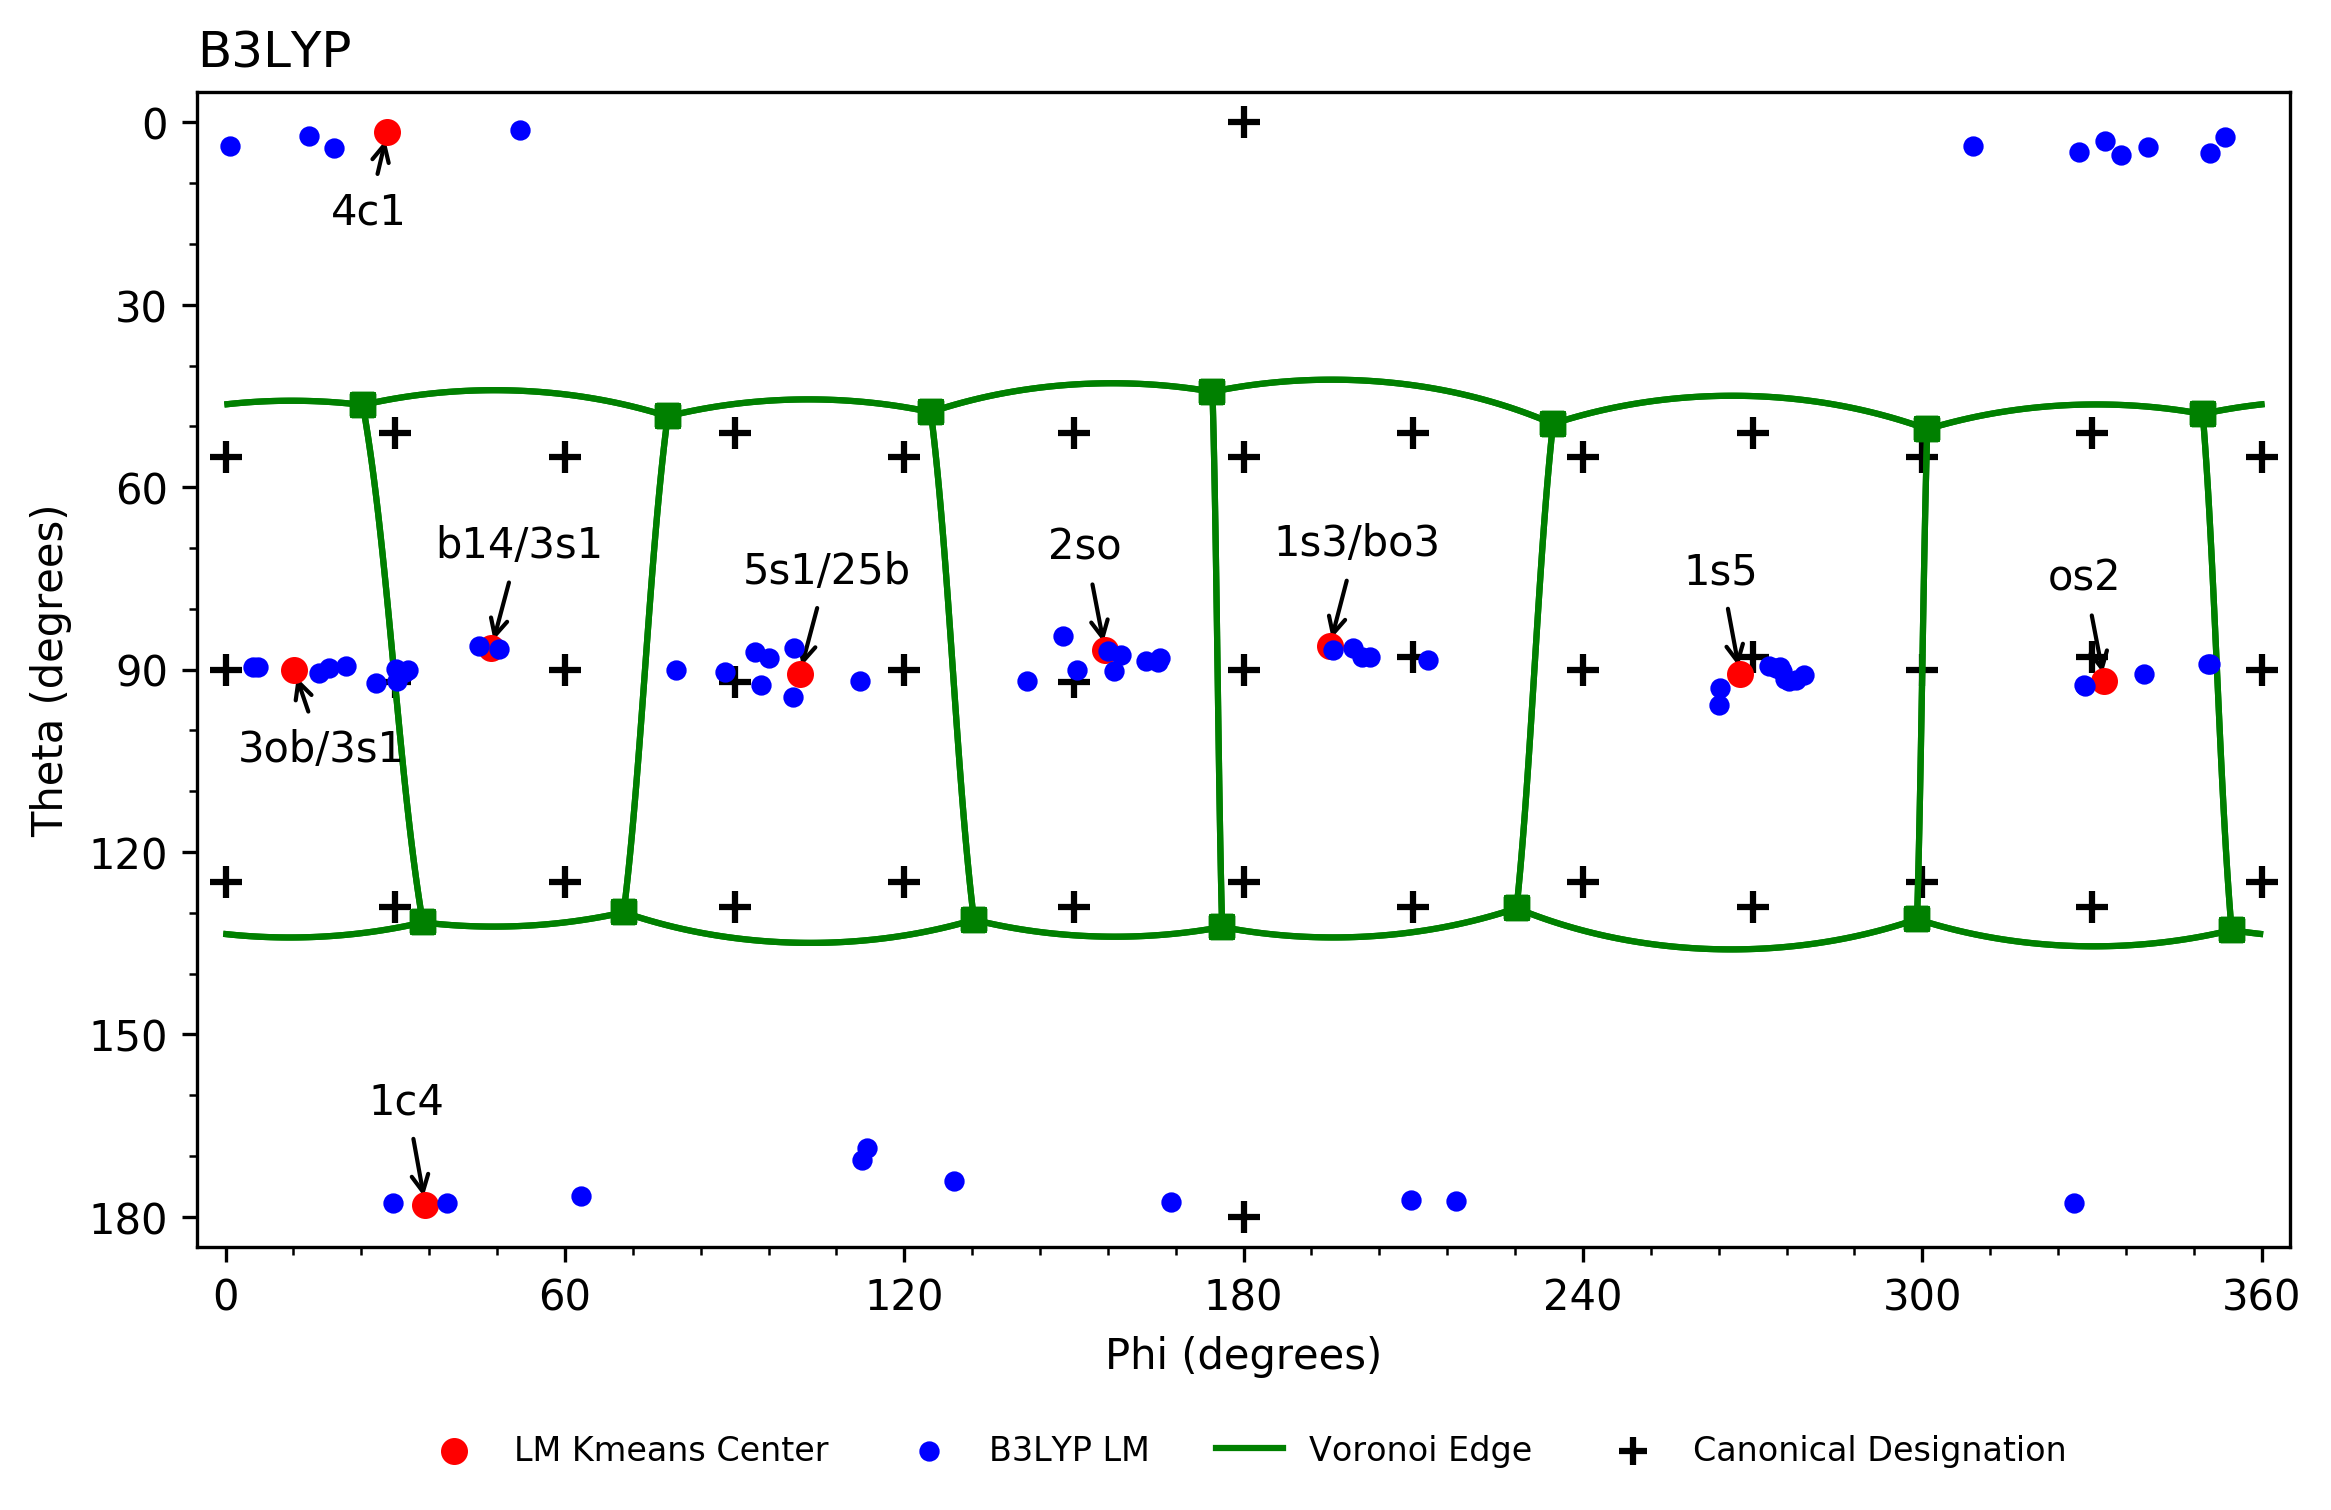
\includegraphics[width=1\textwidth,keepaspectratio]
   	{figures/bxyl/overall/z_dataset-bxyl-LM-B3LYP-all_groupings.png}
   	\caption{B3LYP/6$-$31+G(d,p)}
	\end{subfigure}
	~
	\begin{subfigure}[b]{0.49\textwidth}
	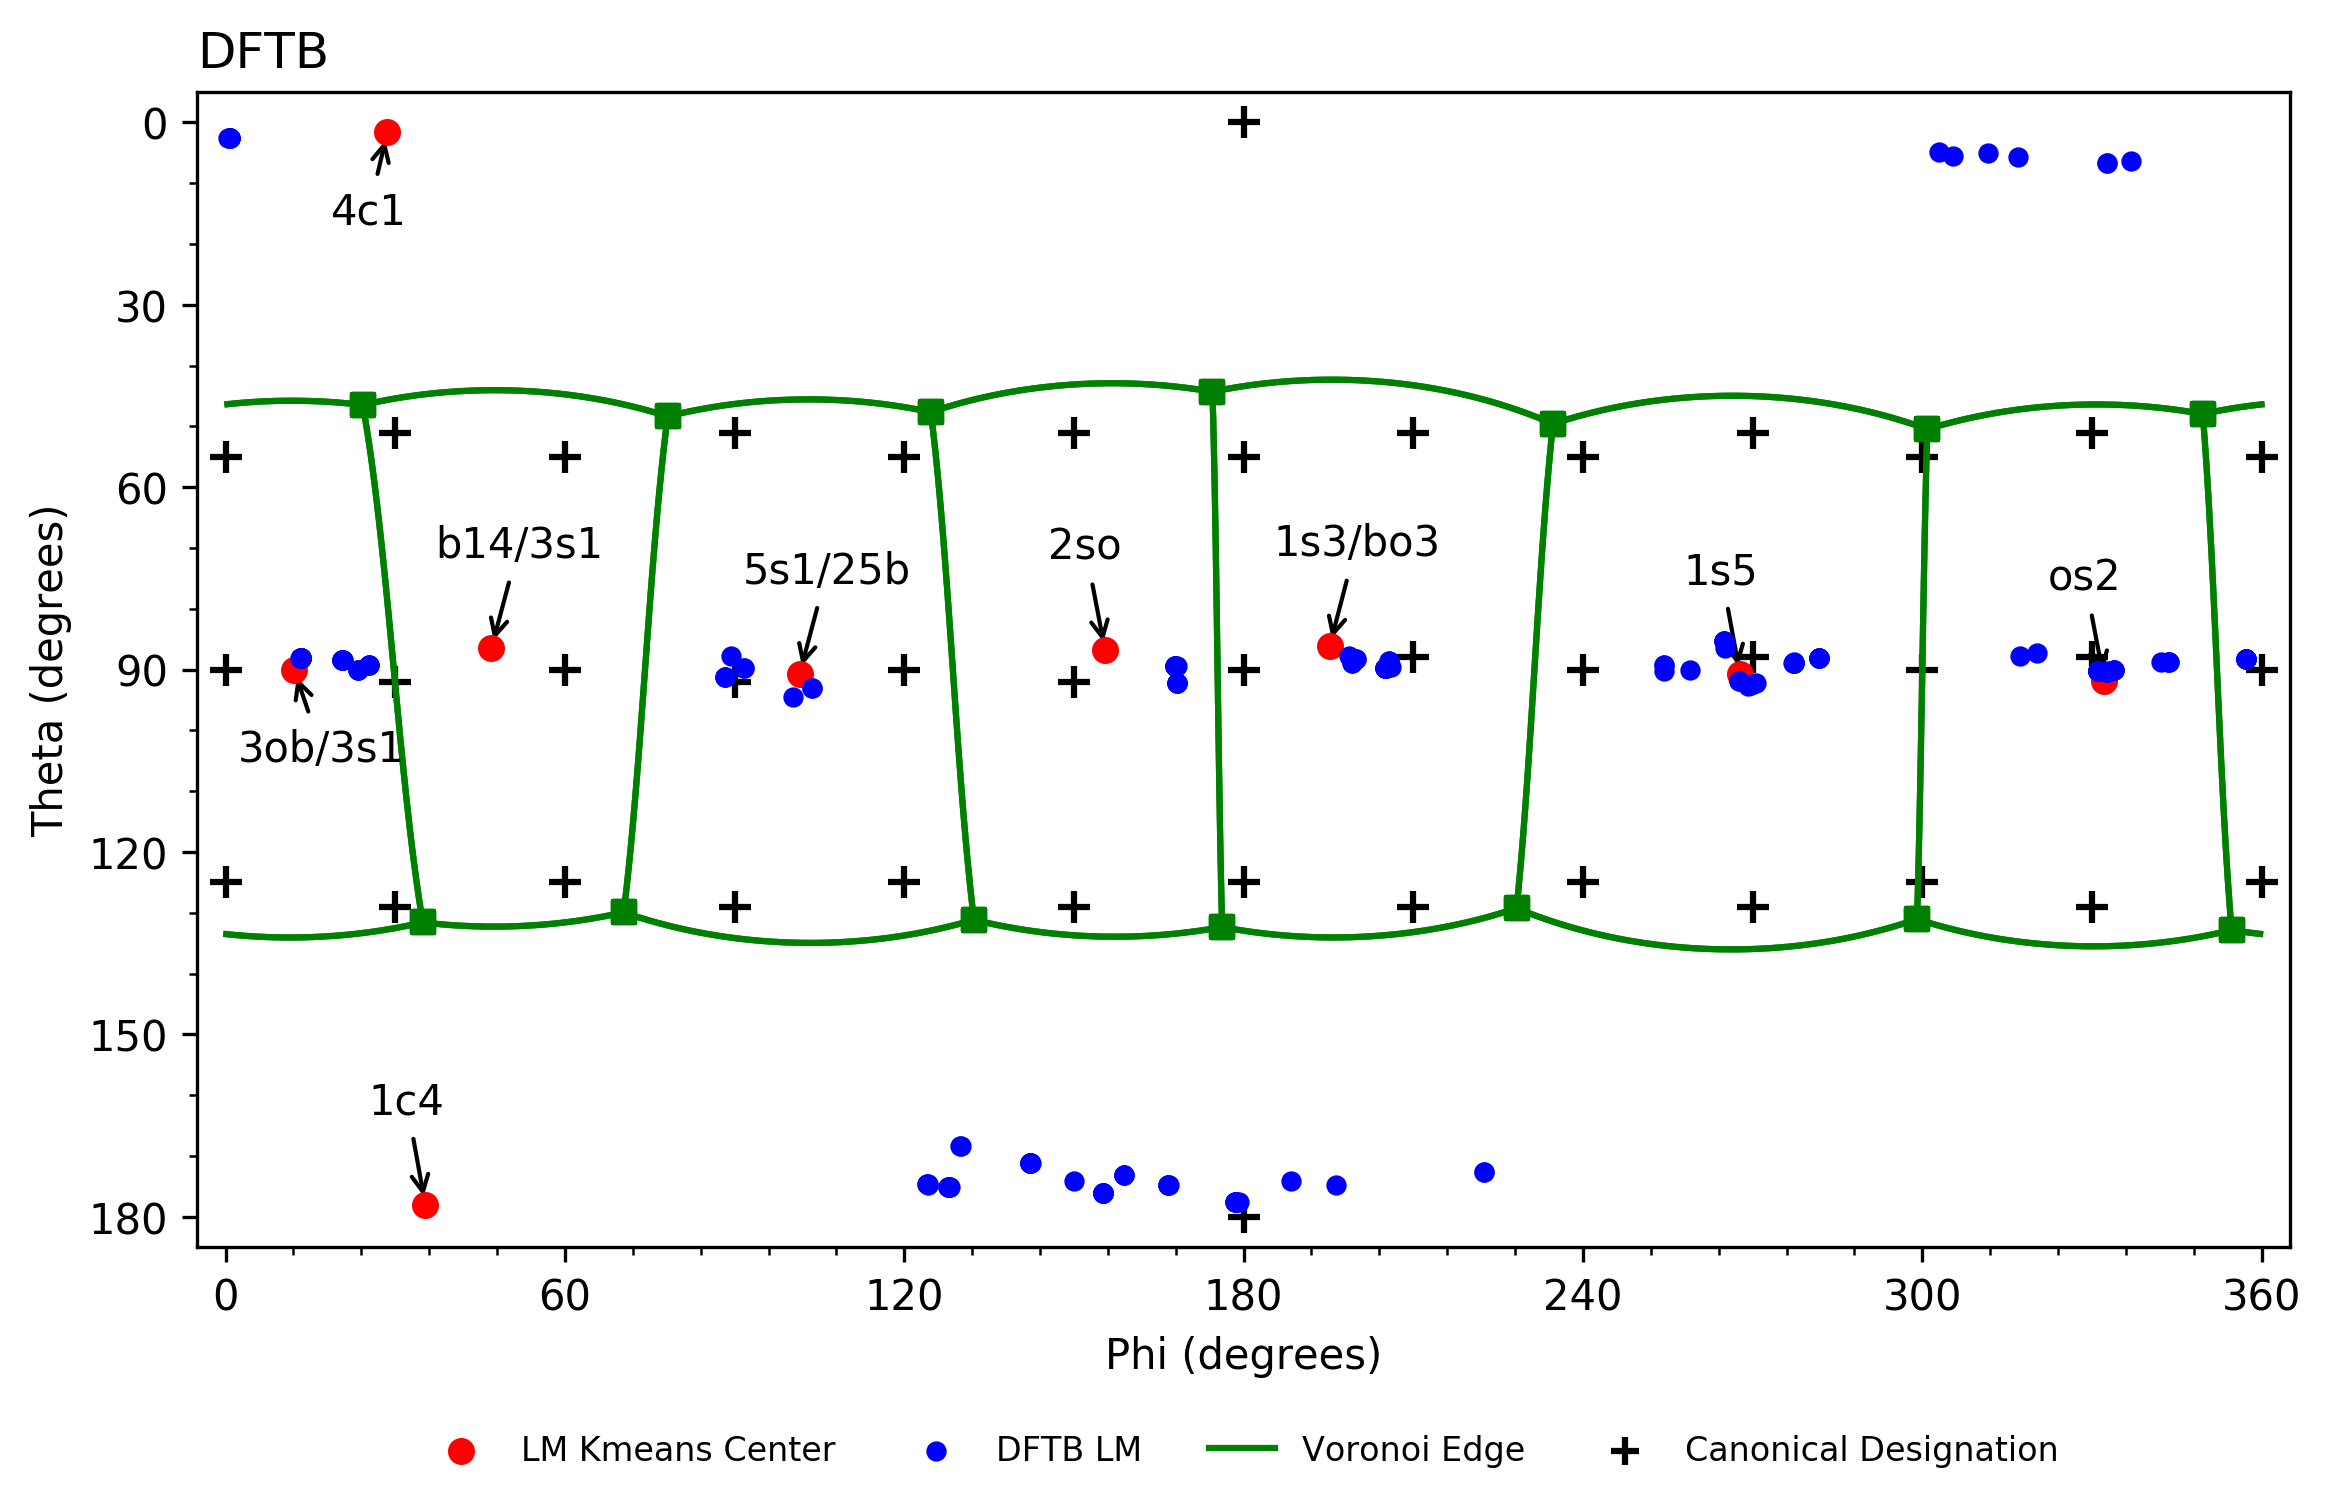
\includegraphics[width=1\textwidth,keepaspectratio]
   	{figures/bxyl/overall/z_dataset-bxyl-LM-DFTB-all_groupings.png}
	\caption{DFTB}
	\end{subfigure}
\end{figure}

\begin{figure}[H]\ContinuedFloat
	\centering
   	\begin{subfigure}[b]{0.49\textwidth}
   	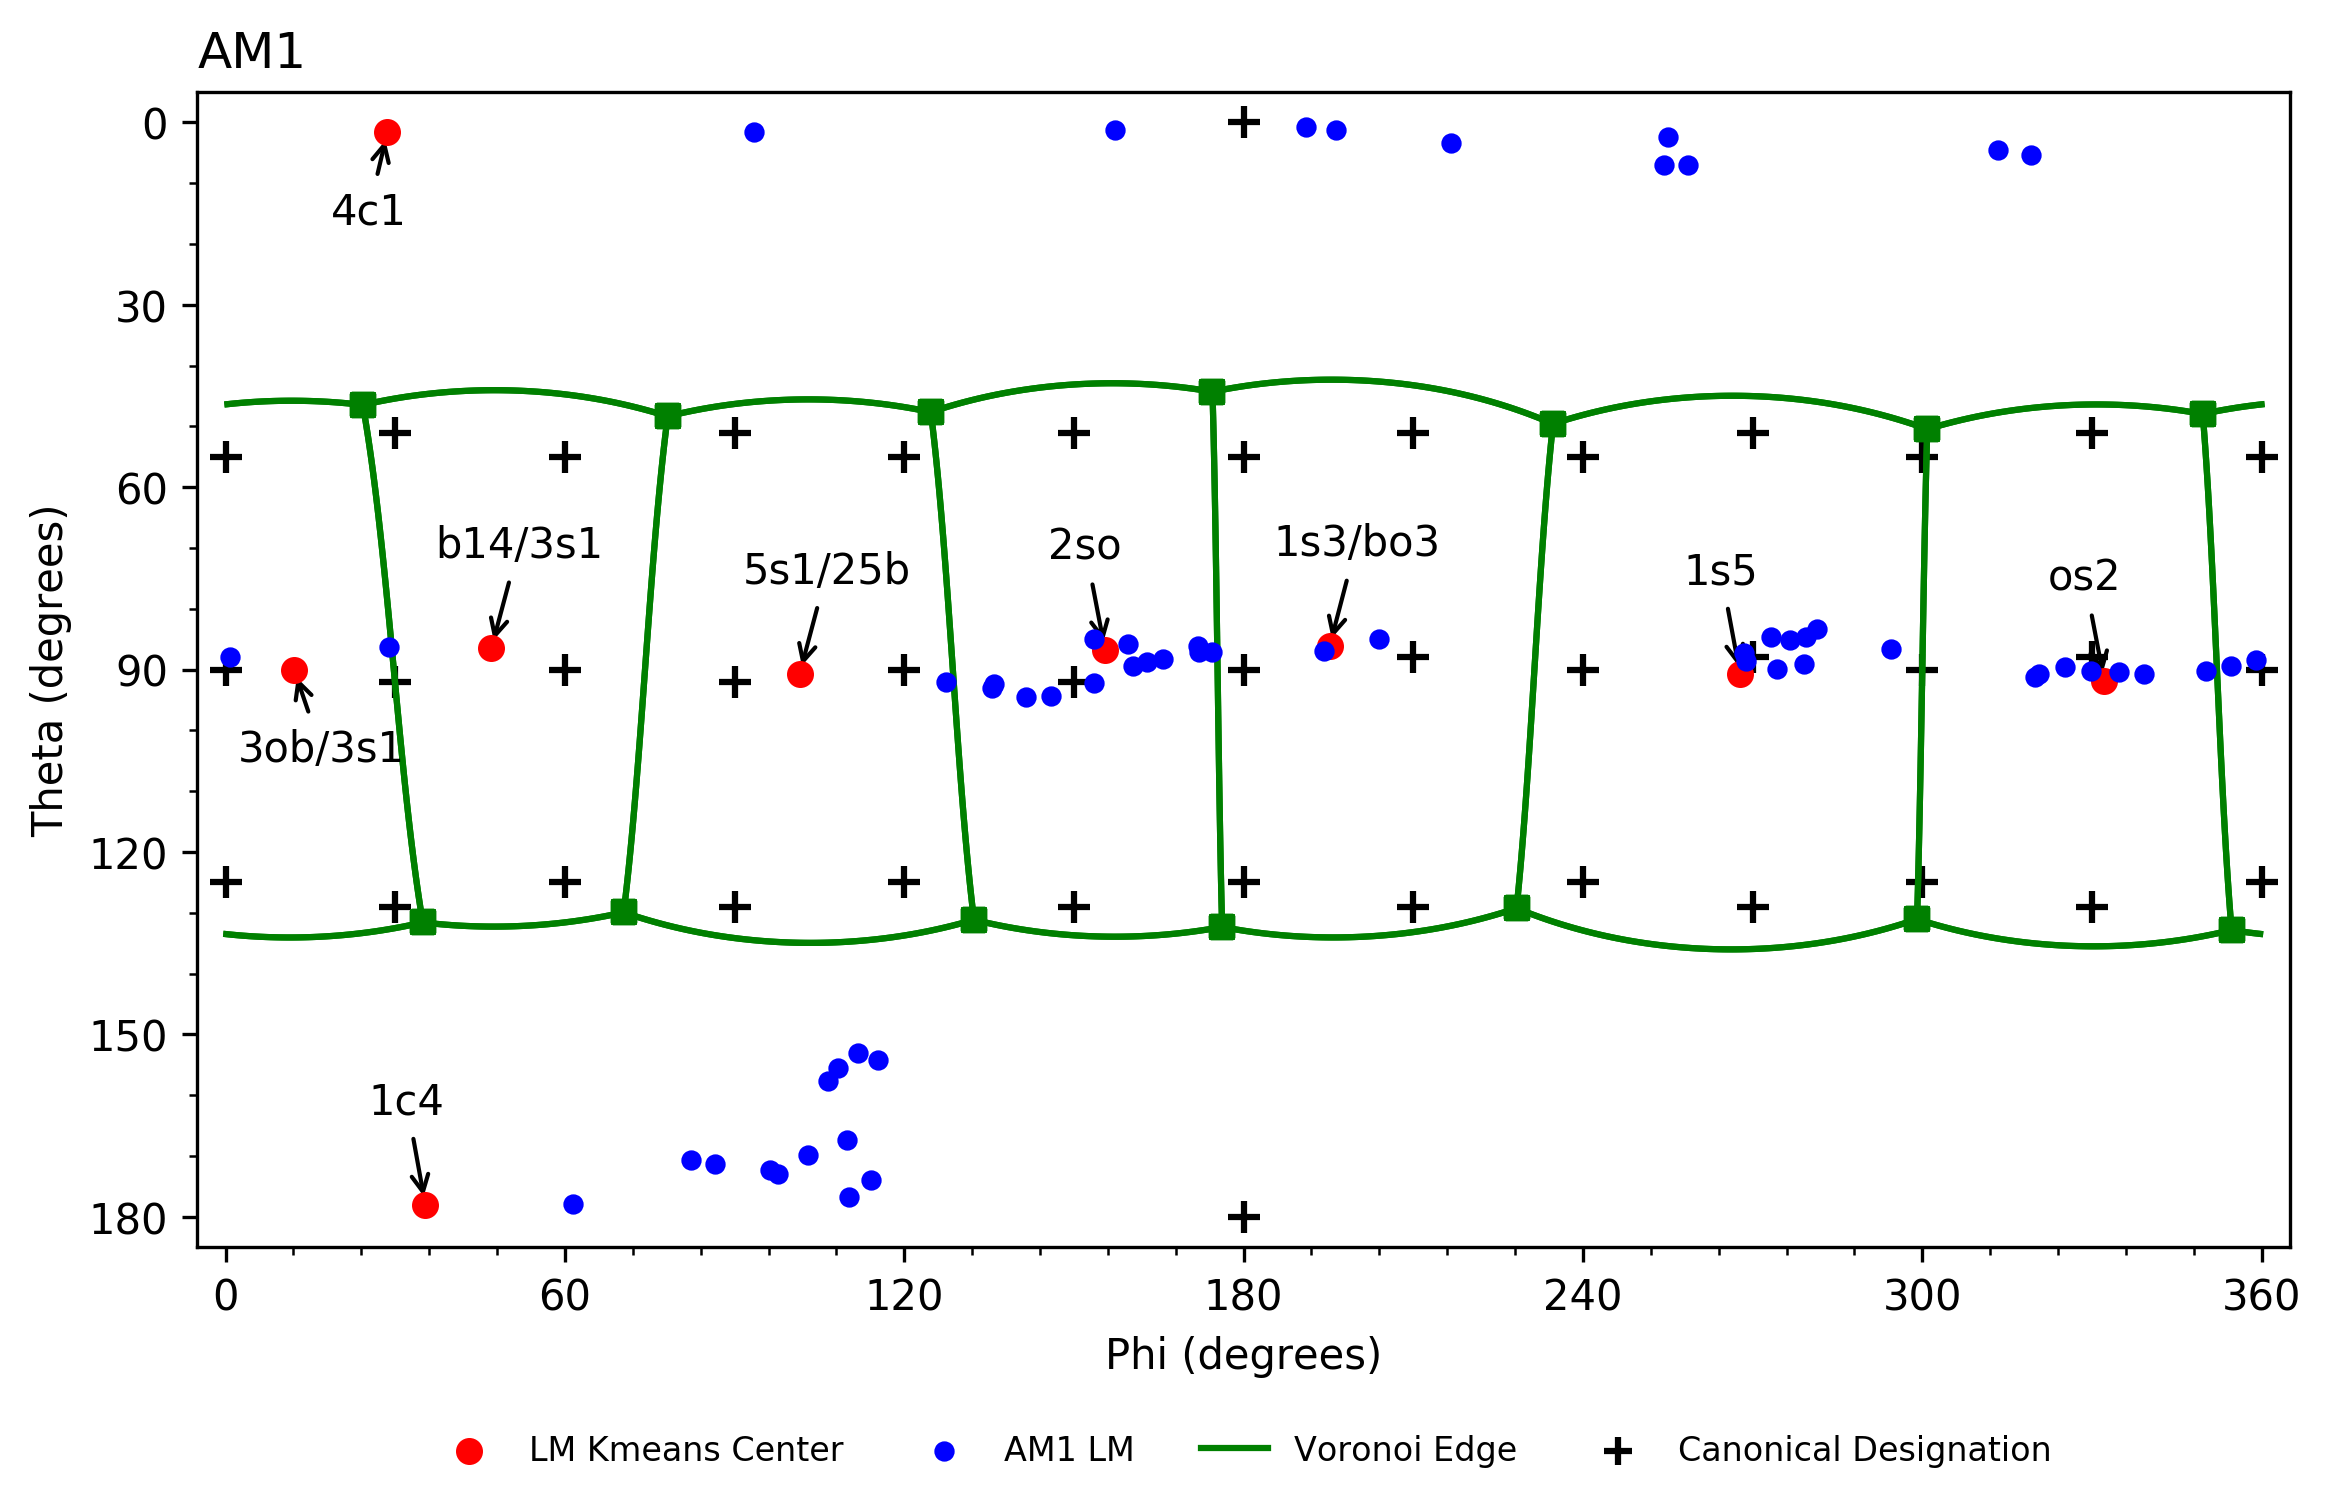
\includegraphics[width=1\textwidth,keepaspectratio]
   	{figures/bxyl/overall/z_dataset-bxyl-LM-AM1-all_groupings.png}
   	\caption{AM1}
	\end{subfigure}
	~
	\begin{subfigure}[b]{0.49\textwidth}
	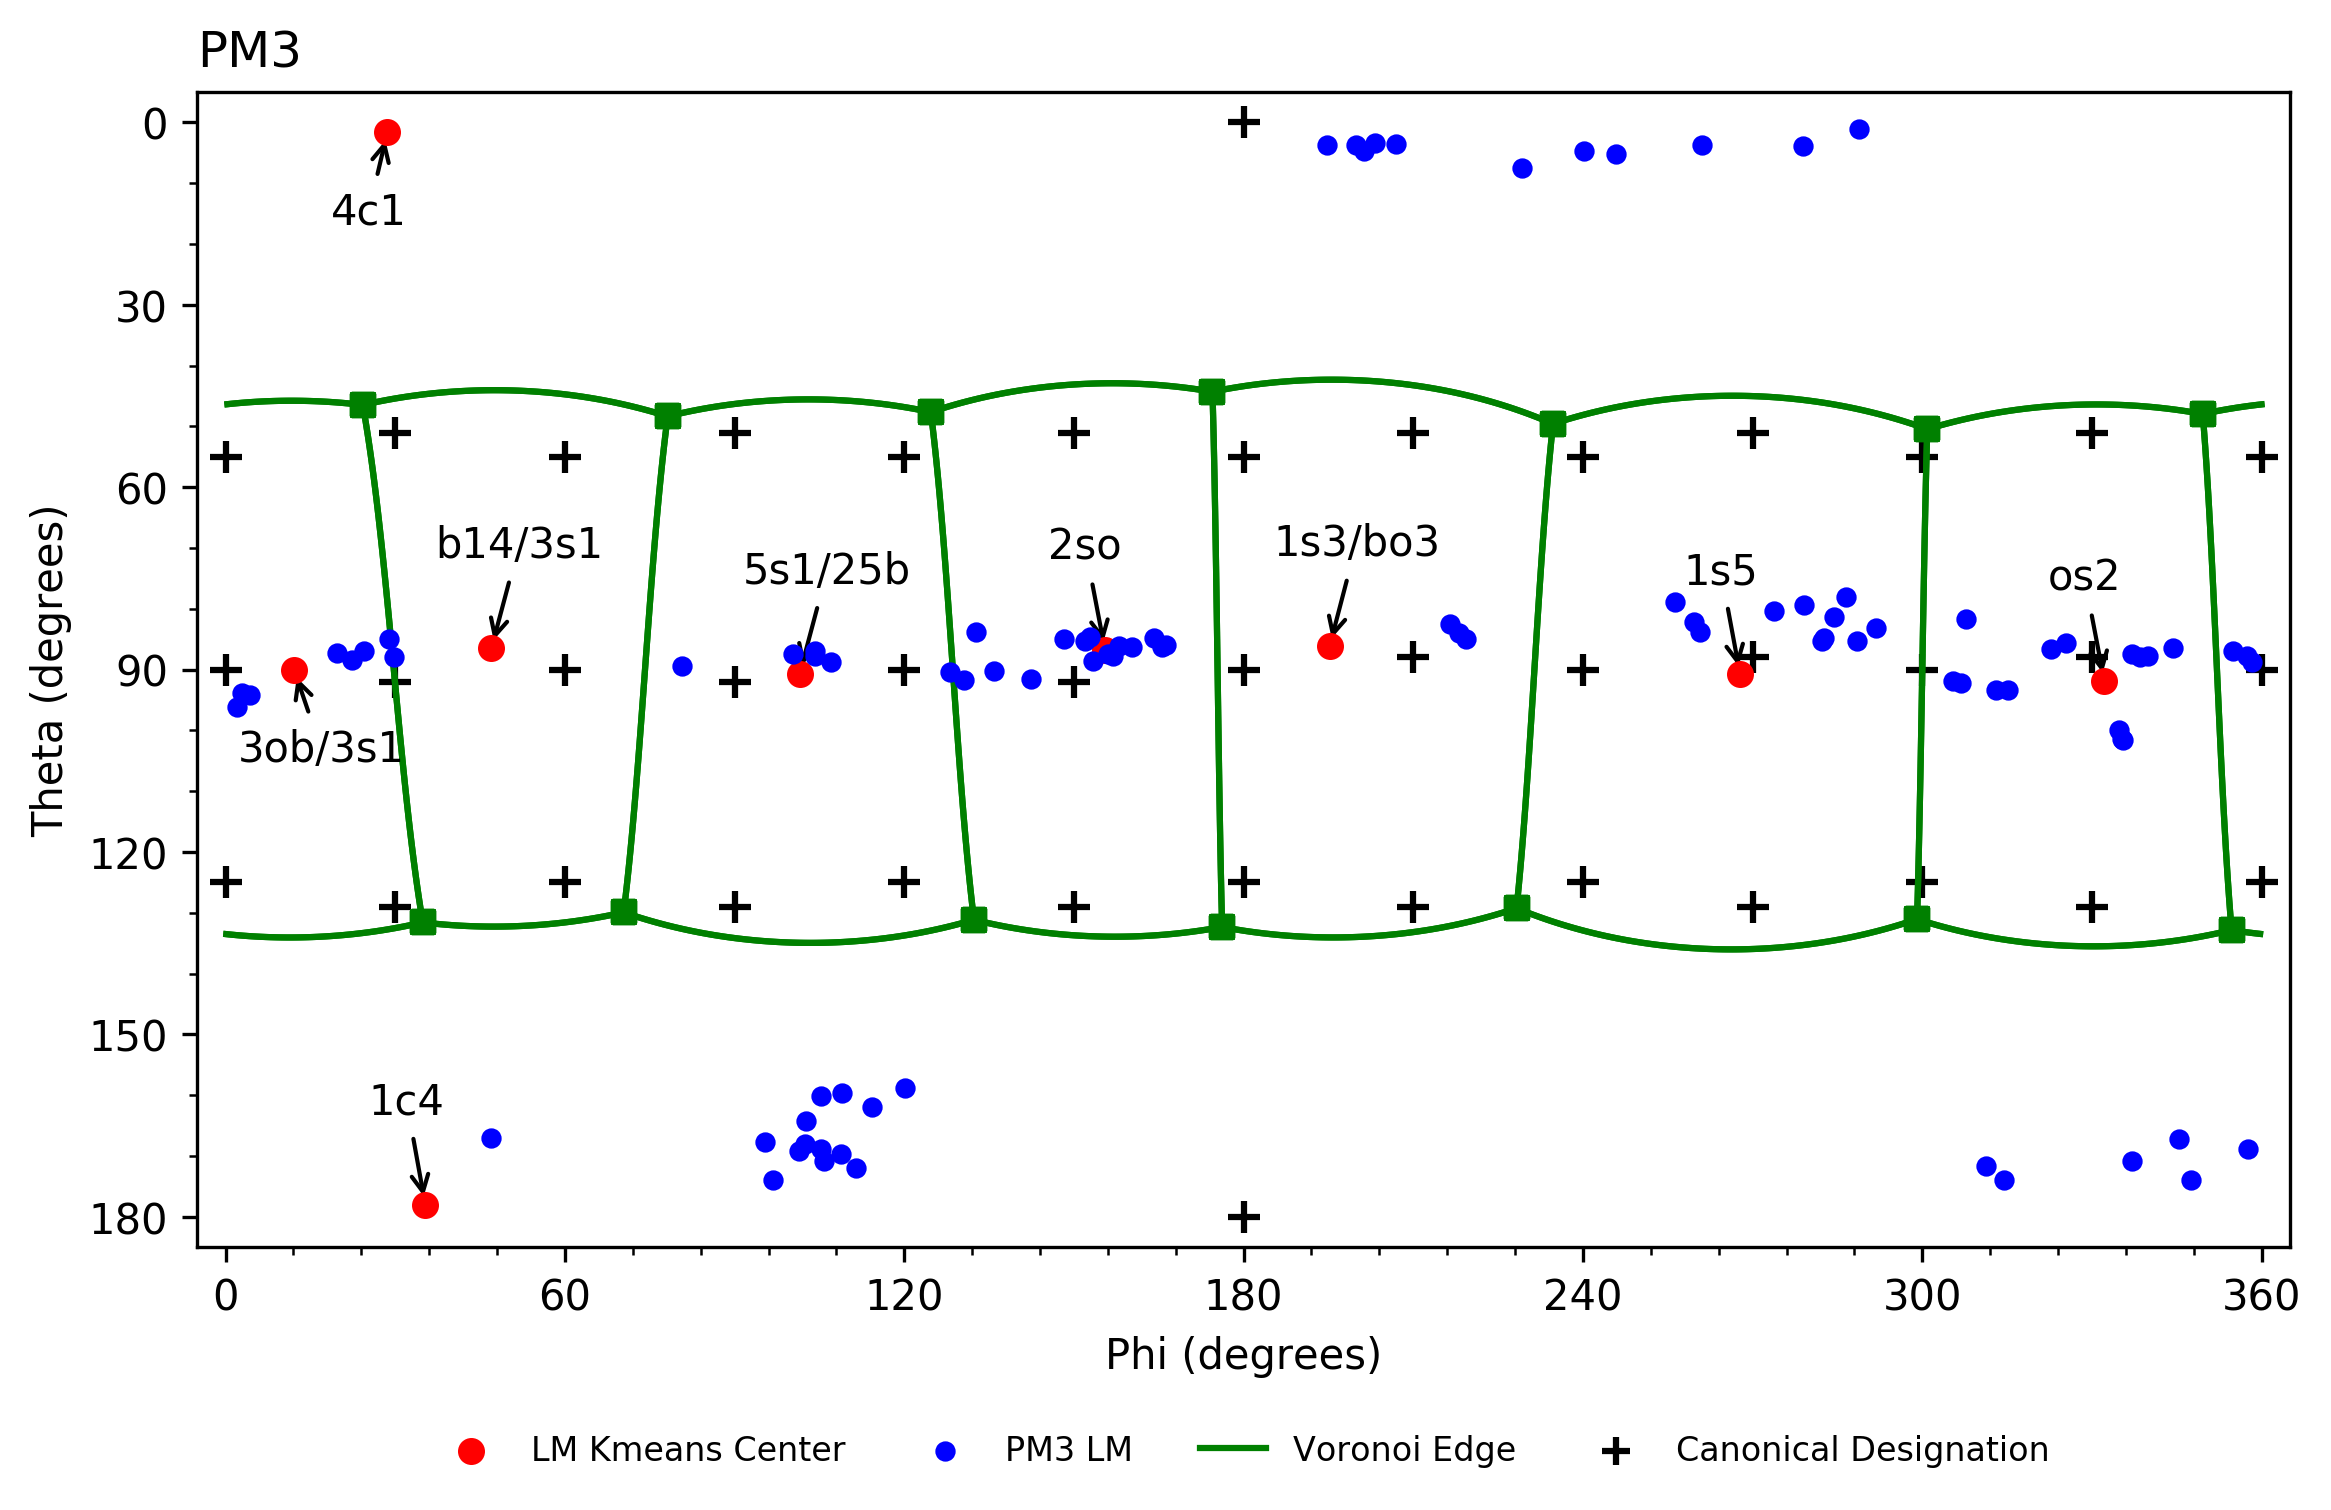
\includegraphics[width=1\textwidth,keepaspectratio]
   	{figures/bxyl/overall/z_dataset-bxyl-LM-PM3-all_groupings.png}
	\caption{PM3}
	\end{subfigure}
\end{figure}

\begin{figure}[H]\ContinuedFloat
	\centering
   	\begin{subfigure}[b]{0.49\textwidth}
   	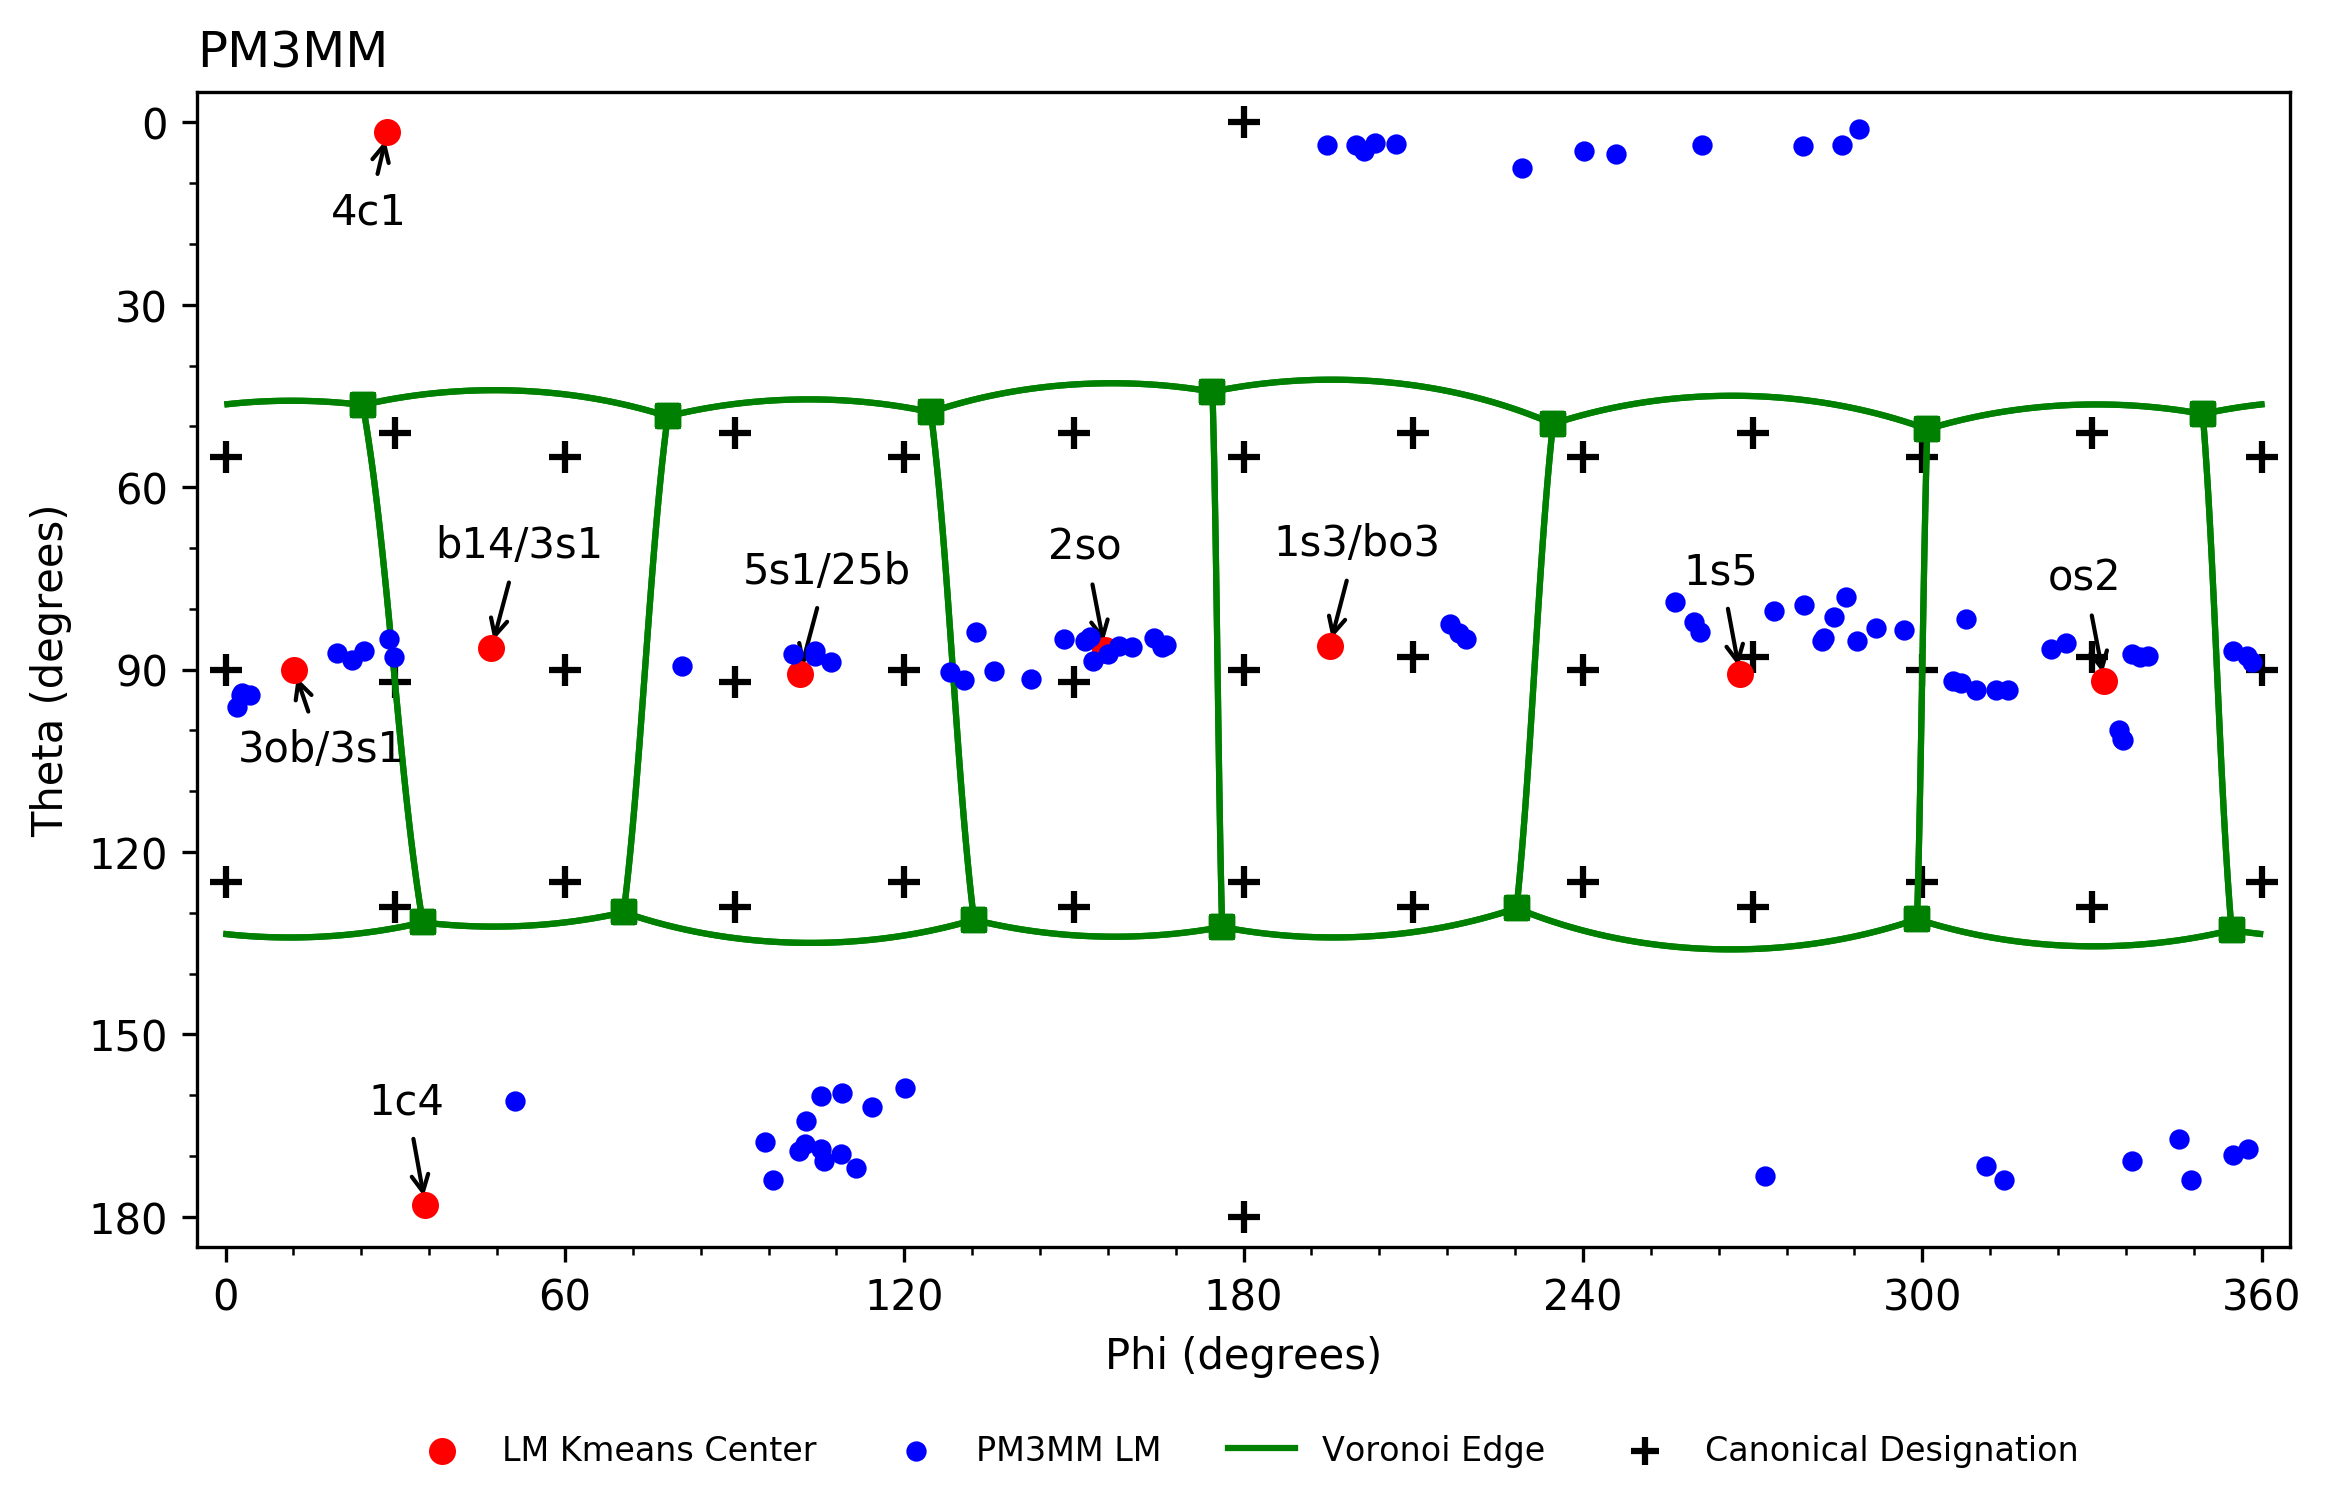
\includegraphics[width=1\textwidth,keepaspectratio]
   	{figures/bxyl/overall/z_dataset-bxyl-LM-PM3MM-all_groupings.png}
   	\caption{PM3MM}
	\end{subfigure}
	~
	\begin{subfigure}[b]{0.49\textwidth}
	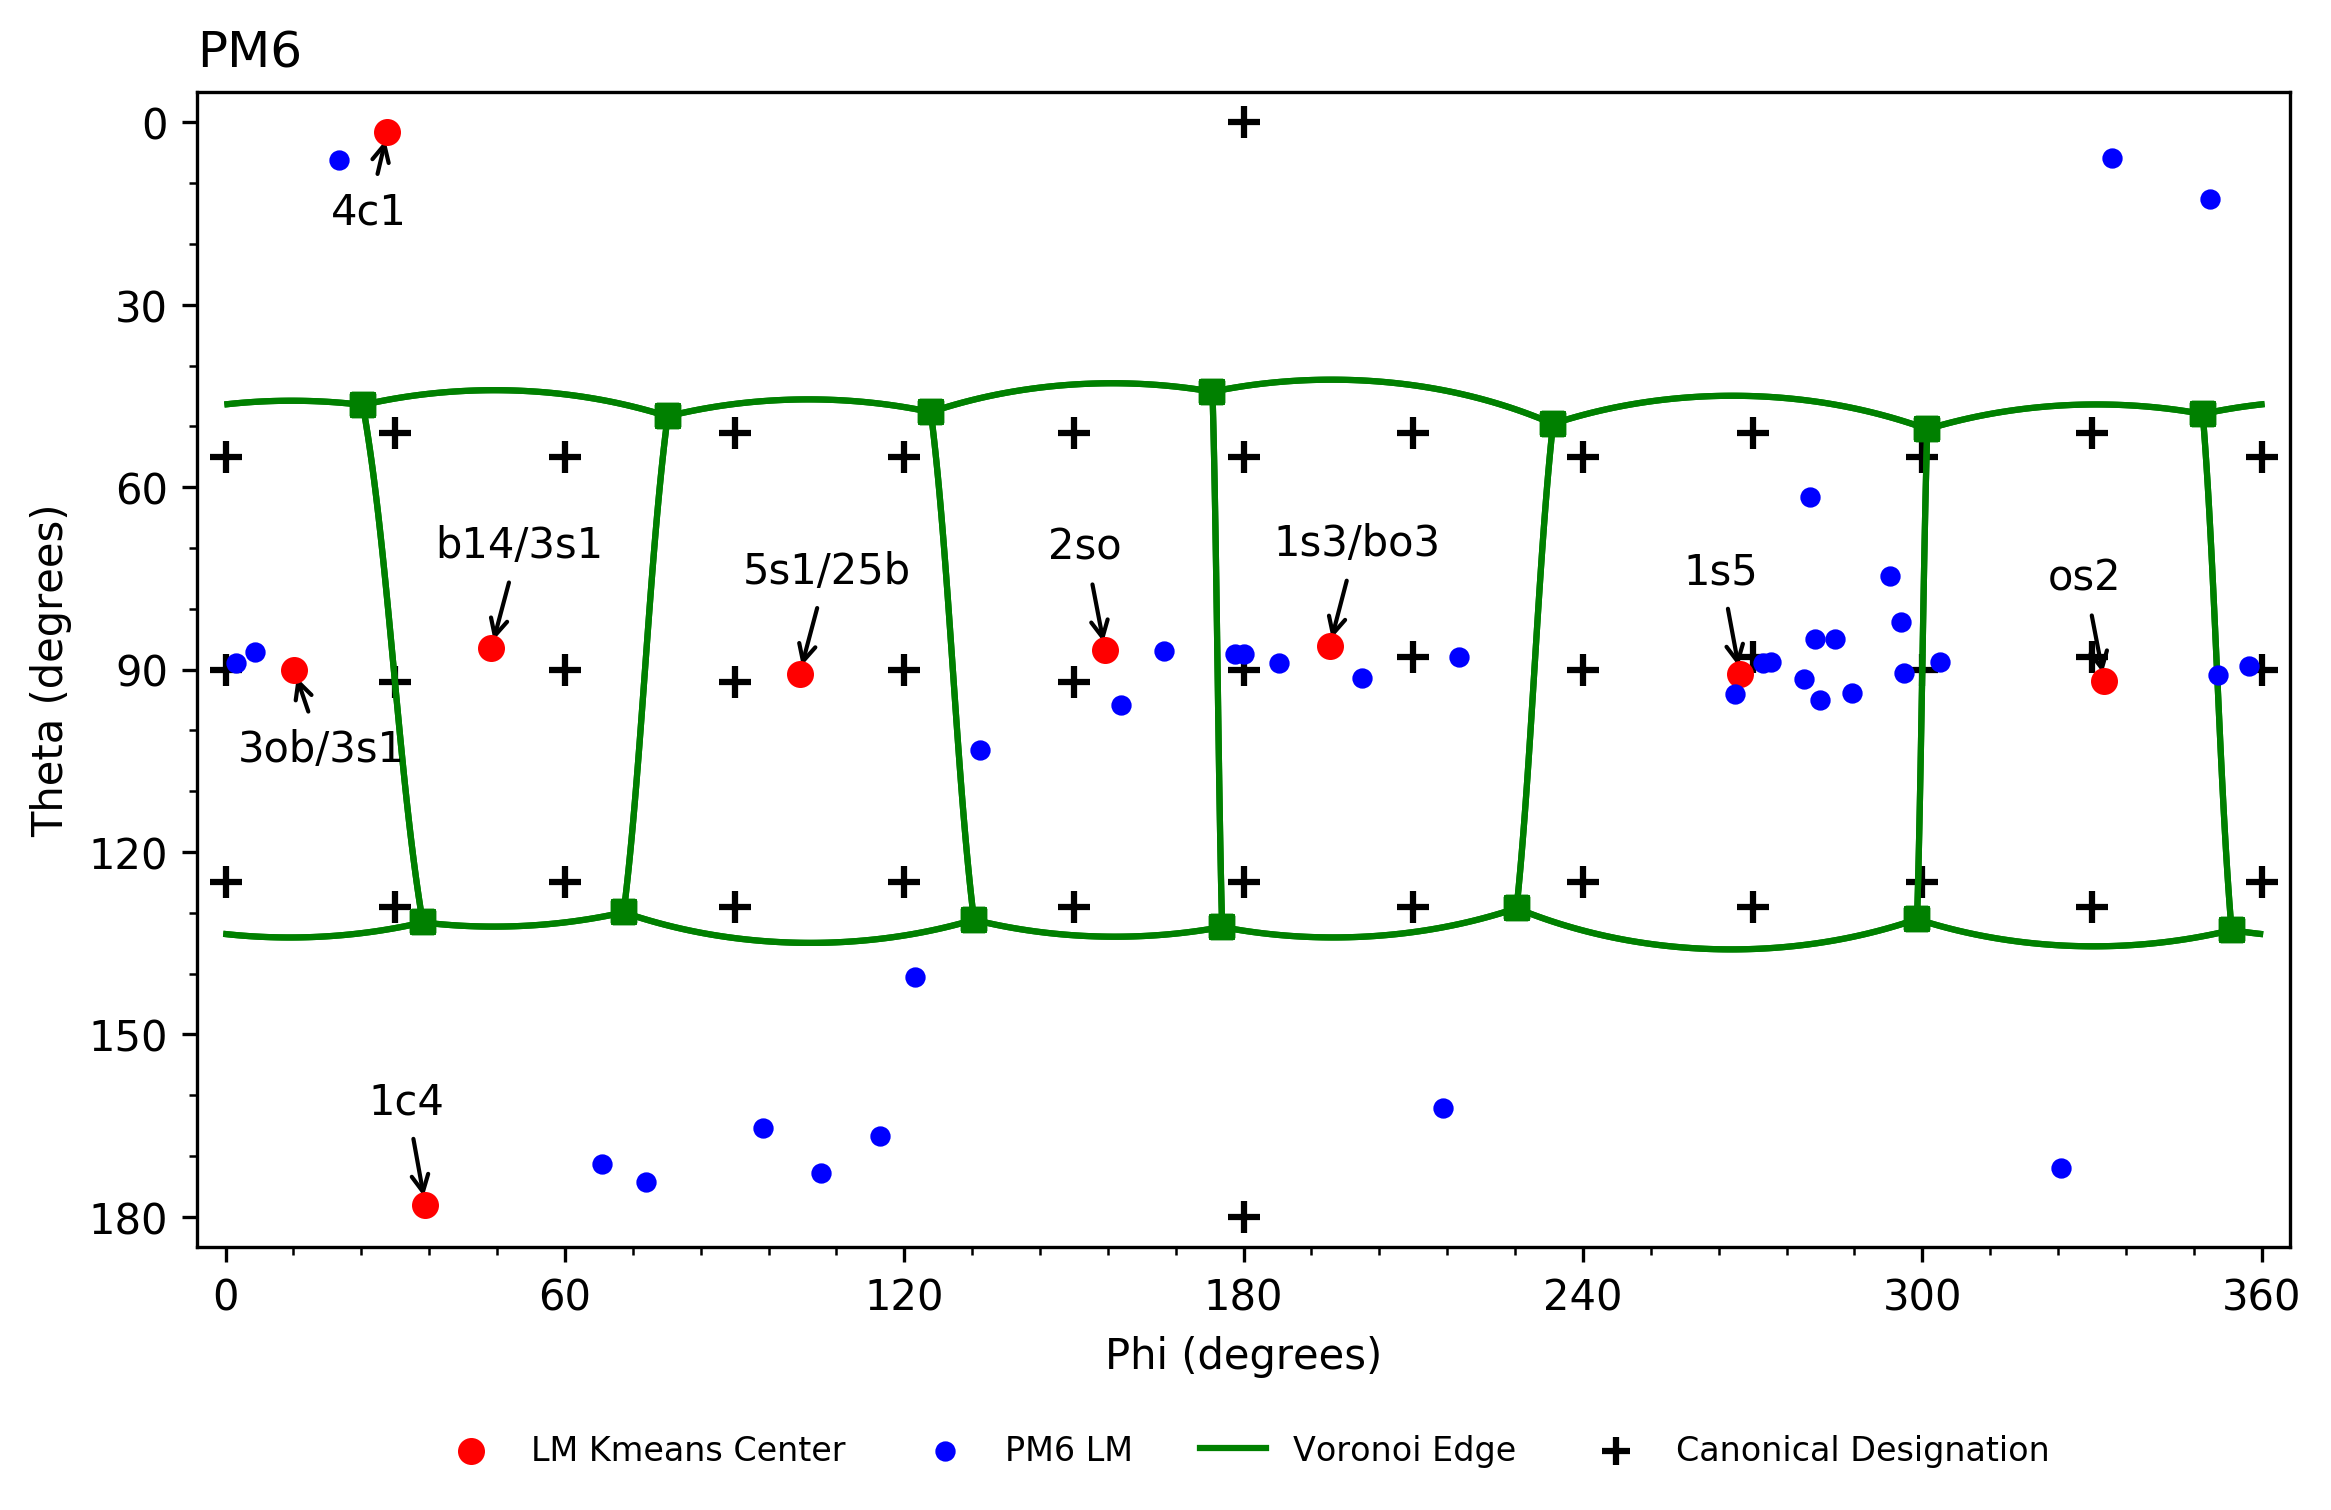
\includegraphics[width=1\textwidth,keepaspectratio]
   	{figures/bxyl/overall/z_dataset-bxyl-LM-PM6-all_groupings.png}
	\caption{PM6}
	\end{subfigure}
\caption{\hl{Insert Caption}}
\label{fig:bxyl-ALL-LM}
\end{figure}



\newpage 
% % % % % % % % % % % 
% % % Beta-glucose % % % 
% % % % % % % % % % % 
\subsection{\textbeta-Glucose}
The last conformational landscape explored was \textbeta-glucose, which contains four hydroxyl groups and one 
hydroxymethyl group. The addition of the hydroxymethyl group increases the diversity in the conformational 
landscape.

\subsubsection{Local Minima Reference Landscape}

%\begin{figure}[h!]
%	\centering
%	\includegraphics[width=\textwidth,height=\textheight,keepaspectratio]
%	{figures/bglc/}
%	\caption{The LM reference landscape for \textbeta-glucose.}
%	\label{fig:bglc-ref-LM}
%\end{figure}


\subsubsection{Transition State Reference Landscape}


%%%%%%%%%%%%%%%%%%%%%%%%%%%%%%%%%%%%%%%%%%%%%%%%%%%%%%%%%%%%%%%%%%%%%%%%
%     										                  REFERENCES                                                                                                    %
%%%%%%%%%%%%%%%%%%%%%%%%%%%%%%%%%%%%%%%%%%%%%%%%%%%%%%%%%%%%%%%%%%%%%%%%
\newpage 
\bibliography{mybib} %You need to replace "rsc" on this line with the name of your .bib file
\bibliographystyle{unsrt}

\end{document}